\documentclass[]{article}
\usepackage{lmodern}
\usepackage{amssymb,amsmath}
\usepackage{ifxetex,ifluatex}
\usepackage{fixltx2e} % provides \textsubscript
\ifnum 0\ifxetex 1\fi\ifluatex 1\fi=0 % if pdftex
  \usepackage[T1]{fontenc}
  \usepackage[utf8]{inputenc}
\else % if luatex or xelatex
  \ifxetex
    \usepackage{mathspec}
  \else
    \usepackage{fontspec}
  \fi
  \defaultfontfeatures{Ligatures=TeX,Scale=MatchLowercase}
\fi
% use upquote if available, for straight quotes in verbatim environments
\IfFileExists{upquote.sty}{\usepackage{upquote}}{}
% use microtype if available
\IfFileExists{microtype.sty}{%
\usepackage{microtype}
\UseMicrotypeSet[protrusion]{basicmath} % disable protrusion for tt fonts
}{}
\usepackage[margin=1in]{geometry}
\usepackage{hyperref}
\hypersetup{unicode=true,
            pdftitle={Generación Curvas de Descarga de las estaciones de monitoreo de la red hídrica de la Asociación de Canalistas del Embalse Recoleta (ACER)},
            pdfborder={0 0 0},
            breaklinks=true}
\urlstyle{same}  % don't use monospace font for urls
\usepackage{graphicx,grffile}
\makeatletter
\def\maxwidth{\ifdim\Gin@nat@width>\linewidth\linewidth\else\Gin@nat@width\fi}
\def\maxheight{\ifdim\Gin@nat@height>\textheight\textheight\else\Gin@nat@height\fi}
\makeatother
% Scale images if necessary, so that they will not overflow the page
% margins by default, and it is still possible to overwrite the defaults
% using explicit options in \includegraphics[width, height, ...]{}
\setkeys{Gin}{width=\maxwidth,height=\maxheight,keepaspectratio}
\IfFileExists{parskip.sty}{%
\usepackage{parskip}
}{% else
\setlength{\parindent}{0pt}
\setlength{\parskip}{6pt plus 2pt minus 1pt}
}
\setlength{\emergencystretch}{3em}  % prevent overfull lines
\providecommand{\tightlist}{%
  \setlength{\itemsep}{0pt}\setlength{\parskip}{0pt}}
\setcounter{secnumdepth}{5}

%%% Use protect on footnotes to avoid problems with footnotes in titles
\let\rmarkdownfootnote\footnote%
\def\footnote{\protect\rmarkdownfootnote}

%%% Change title format to be more compact
\usepackage{titling}

% Create subtitle command for use in maketitle
\newcommand{\subtitle}[1]{
  \posttitle{
    \begin{center}\large#1\end{center}
    }
}

\setlength{\droptitle}{-2em}
  \title{Generación Curvas de Descarga de las estaciones de telemetría de la red hídrica de la Asociación de Canalistas del Embalse Recoleta (ACER)}
  \pretitle{\vspace{\droptitle}\centering\huge}
  \posttitle{\par}
  \author{}
  \preauthor{}\postauthor{}
  \date{}
  \predate{}\postdate{}

\usepackage{geometry}
\geometry{letterpaper}
\usepackage{graphicx}
\usepackage{amssymb}
\usepackage{hyperref}
\usepackage{titlesec}
\usepackage{appendix}  
\usepackage{booktabs}
\usepackage{longtable}
\usepackage{multirow}
\usepackage{subcaption}
\usepackage{rotating}

\usepackage{fontspec,xltxtra,xunicode}
\defaultfontfeatures{Mapping=tex-text}
\setmainfont[		
 BoldFont={Century Gothic Bold}, 
 ItalicFont={Century Gothic Italic},
 BoldItalicFont={Century Gothic Bold Italic}
 ]{Century Gothic}

\renewcommand{\figurename}{Figura}
\renewcommand{\tablename}{Cuadro} 
\renewcommand{\contentsname}{Tabla de contenidos\\} 
\renewcommand{\listfigurename}{Índice de figuras\\}
\renewcommand{\listtablename}{Índice de cuadros\\} 
\renewcommand{\appendixname}{Anexos}
\renewcommand{\appendixtocname}{Anexos}
\renewcommand{\appendixpagename}{Anexos}


\titleformat*{\section}{\normalsize\bfseries}
\titleformat*{\subsection}{\normalsize\bfseries}
\titleformat*{\subsubsection}{\normalsize\bfseries}

\usepackage{fancyvrb}
\newcommand{\VerbBar}{|}
\newcommand{\VERB}{\Verb[commandchars=\\\{\}]}
\DefineVerbatimEnvironment{Highlighting}{Verbatim}{commandchars=\\\{\}}
% Add ',fontsize=\small' for more characters per line
\usepackage{color}
\usepackage{framed}
\usepackage{tabulary}
\definecolor{shadecolor}{RGB}{248,248,248}
\newenvironment{Shaded}{\begin{snugshade}}{\end{snugshade}}
\newcommand{\KeywordTok}[1]{\textcolor[rgb]{0.13,0.29,0.53}{\textbf{#1}}}
\newcommand{\DataTypeTok}[1]{\textcolor[rgb]{0.13,0.29,0.53}{#1}}
\newcommand{\DecValTok}[1]{\textcolor[rgb]{0.00,0.00,0.81}{#1}}
\newcommand{\BaseNTok}[1]{\textcolor[rgb]{0.00,0.00,0.81}{#1}}
\newcommand{\FloatTok}[1]{\textcolor[rgb]{0.00,0.00,0.81}{#1}}
\newcommand{\ConstantTok}[1]{\textcolor[rgb]{0.00,0.00,0.00}{#1}}
\newcommand{\CharTok}[1]{\textcolor[rgb]{0.31,0.60,0.02}{#1}}
\newcommand{\SpecialCharTok}[1]{\textcolor[rgb]{0.00,0.00,0.00}{#1}}
\newcommand{\StringTok}[1]{\textcolor[rgb]{0.31,0.60,0.02}{#1}}
\newcommand{\VerbatimStringTok}[1]{\textcolor[rgb]{0.31,0.60,0.02}{#1}}
\newcommand{\SpecialStringTok}[1]{\textcolor[rgb]{0.31,0.60,0.02}{#1}}
\newcommand{\ImportTok}[1]{#1}
\newcommand{\CommentTok}[1]{\textcolor[rgb]{0.56,0.35,0.01}{\textit{#1}}}
\newcommand{\DocumentationTok}[1]{\textcolor[rgb]{0.56,0.35,0.01}{\textbf{\textit{#1}}}}
\newcommand{\AnnotationTok}[1]{\textcolor[rgb]{0.56,0.35,0.01}{\textbf{\textit{#1}}}}
\newcommand{\CommentVarTok}[1]{\textcolor[rgb]{0.56,0.35,0.01}{\textbf{\textit{#1}}}}
\newcommand{\OtherTok}[1]{\textcolor[rgb]{0.56,0.35,0.01}{#1}}
\newcommand{\FunctionTok}[1]{\textcolor[rgb]{0.00,0.00,0.00}{#1}}
\newcommand{\VariableTok}[1]{\textcolor[rgb]{0.00,0.00,0.00}{#1}}
\newcommand{\ControlFlowTok}[1]{\textcolor[rgb]{0.13,0.29,0.53}{\textbf{#1}}}
\newcommand{\OperatorTok}[1]{\textcolor[rgb]{0.81,0.36,0.00}{\textbf{#1}}}
\newcommand{\BuiltInTok}[1]{#1}
\newcommand{\ExtensionTok}[1]{#1}
\newcommand{\PreprocessorTok}[1]{\textcolor[rgb]{0.56,0.35,0.01}{\textit{#1}}}
\newcommand{\AttributeTok}[1]{\textcolor[rgb]{0.77,0.63,0.00}{#1}}
\newcommand{\RegionMarkerTok}[1]{#1}
\newcommand{\InformationTok}[1]{\textcolor[rgb]{0.56,0.35,0.01}{\textbf{\textit{#1}}}}
\newcommand{\WarningTok}[1]{\textcolor[rgb]{0.56,0.35,0.01}{\textbf{\textit{#1}}}}
\newcommand{\AlertTok}[1]{\textcolor[rgb]{0.94,0.16,0.16}{#1}}
\newcommand{\ErrorTok}[1]{\textcolor[rgb]{0.64,0.00,0.00}{\textbf{#1}}}
\newcommand{\NormalTok}[1]{#1}
\usepackage{graphicx,grffile}
\makeatletter
\def\maxwidth{\ifdim\Gin@nat@width>\linewidth\linewidth\else\Gin@nat@width\fi}
\def\maxheight{\ifdim\Gin@nat@height>\textheight\textheight\else\Gin@nat@height\fi}
\makeatother
\usepackage{booktabs}
\usepackage{longtable}
\usepackage{array}
\usepackage{multirow}
\usepackage[table]{xcolor}
\usepackage{wrapfig}
\usepackage{float}
\usepackage{colortbl}
\usepackage{pdflscape}
\usepackage{tabu}
\usepackage{threeparttable}
\usepackage[normalem]{ulem}
\usepackage[none]{hyphenat}

\begin{document}
\sloppy 

\begin{titlepage}

\begin{figure}
 \centering \vspace*{1in}
  \includegraphics[width=.3\textwidth]{Logo/horizsinfondo.png}
  \vspace*{1in}
\end{figure}
\maketitle \thispagestyle{empty} \vspace*{2.5in}
\begin{center}
    \fontsize{14}{0} \selectfont{Febrero 2018}
\end{center}

\begin{figure}
  \centering
\begin{subfigure}{.2\textwidth}
  \includegraphics[width=\textwidth]{Logo/corfo.jpg}
\end{subfigure}
\hfill
\begin{subfigure}{.2\textwidth}
  \includegraphics[width=\textwidth]{Logo/LOGO_RECOLETA.png}
\end{subfigure}

\end{figure}

\end{titlepage}

\begin{titlepage}


\textbf{ENTIDAD MANDANTE } 

\vspace*{.1in} Asociación de Canalistas del Embalse Recoleta (ACER)\vspace*{.4in} 

\textbf{ENTIDAD EJECUTORA} 

\vspace*{.1in} RAIZ Consultores

\vfill \textbf{Ovalle}
\\ \textbf{Febrero de 2018} 
\\ \textbf{Región de Coquimbo}
\\ \textbf{Chile} 

\end{titlepage}

\newpage 

\begin{titlepage}
\centering
\textbf{EQUIPO DE TRABAJO}\\

\begin{figure}[!h]
 \centering
   \vspace*{.5in}
      \includegraphics[width=.3\textwidth]{Logo/horizsinfondo.png}
   \vspace*{.5in}
\end{figure}

\textbf{ENTIDAD EJECUTORA}\\
\bigskip 
\textbf{RAIZ Consultores}\\
\bigskip 
\textbf{Ing. Agr. Gonzalo Rojas Fernández}\\
Director de Proyecto\\
\bigskip 
\textbf{Ing. Agr. Aldo Tapia Araya}\\
Ingeniero en Desarrollo\\
\bigskip 
\textbf{Ing. Agr. Erick Millón Henríquez}\\
Ingeniero de Terreno\\
\bigskip 
\textbf{Luis Torrejón Cortés}\\
Equipo de Terreno\\
\bigskip 
\textbf{Francisco Tapia Cortés}\\
Equipo de Terreno\\
\bigskip 
\textbf{Dr. Pablo Álvarez Latorre}\\
Consultor\\

\vspace*{2in}
\begin{center}
\textbf{CONTRAPARTE TÉCNICA}\\
\textbf{Departamento de Administración}\\
\textbf{Asociación de Canalistas del Embalse Recoleta}\\
\textbf{Región de Coquimbo}\\

\end{center}

\end{titlepage}

\tableofcontents

\newpage 
\listoffigures
\newpage 
\listoftables

\newpage 
\section{Introducción}\label{introduccion}

Bajo la ejecución del proyecto \emph{Mejoramiento y fortalecimiento de
las capacidades de gestión integrada y administrativas, para el
desarrollo de una cultura del agua, y adaptación al cambio climático a
través del buen uso del recurso hídrico de la Asociación de Canalistas
del Embalse Recoleta}, se le ha encargado a esta consultora, el
desarrollo de las curvas de descarga de las estaciones de monitoreo de
la red hídrica, pertenecientes a la Asociación de Canalistas del Embalse
Recoleta (ACER).

Para el desarrollo de cada una de las curvas de descarga, se trabajó en
base a la información proporcionada por el Departamento de Desarrollo y
por la Administración de la organización, los cuales consideró el
Sistema de Información Geográfica (SIG) de la red hídrica; información
de operación, información de gestión, información actualizada de algunas
curvas de descarga de estaciones de monitoreo generadas en proyectos
anteriores, entre otros.

Los aforos realizados para la generación de las curvas, fueron
ejecutados bajo los criterios definidos en el \emph{Manual Auto
instructivo de aforo en canales no revestidos -- Ley Nº18.450}, de la
Comisión Nacional de Riego (CNR). En el documento se establecen las
bases técnicas para la realización de aforos, bajo los criterios
técnicos definidos por el organismo, y que, a su vez, permiten validar
los datos para poder postularlos a proyectos de mejoramiento de canales.

La realización de los aforos en cada punto, además de cumplir con los
criterios técnicos de la CNR, fueron complementados con el uso de
herramientas tecnologías, como la desarrollada por el Laboratorio de
Prospección, Monitoreo y Modelación de Recursos Agrícolas y Ambientales
(PROMMRA) de la Universidad de La Serena, laboratorio que diseñó una
planilla automática para el cálculo de caudales denominada PROMMRA --
QCANAL, que cumple con los criterios definidos por la CNR. Esta
herramienta permite realizar en terreno los cálculos para la
determinación de caudales, permitiendo reducir la incertidumbre de los
datos levantados.

\newpage

\section{Procedimiento de aforo}\label{procedimiento-de-aforo}

El desarrollo de las curvas se realizó a partir de los volúmenes que
están siendo entregados por la Asociación de Canalistas del Embalse
Recoleta (ACER) al inicio del período de mayor demanda para riego. Esta
condición hace que gran parte de las curvas de descarga tomadas en cada
punto de la red de estaciones telemétricas, se compongan de alturas y
por ende de caudales mayores. Sin embargo, en algunos puntos de aforo se
pudo manipular a discreción las compuertas de entrega y por lo tanto
generar una distribución uniforme de alturas y caudales dentro de la
curva de descarga generada.

Para la realización de las curvas de descarga se ejecutaron aforos a
distintas alturas de lámina de agua en las estaciones de telemetría, los
cuales permitieron relacionar la altura de la lámina de agua con el
caudal pasante.

Previo a la ejecución de los aforos, es necesario seleccionar la sección
donde se va realizar la medición. Esta sección debe cumplir con ciertos
requisitos técnicos y logísticos para obtener una medición confiable,
dentro de lo que destaca la ubicación de esta, la que debe ser en un
tramo recto del cauce, donde se aprecien líneas de flujo uniformes y
paralelas a los márgenes de la corriente, con una pendiente longitudinal
constante (evitar tramos con quiebres fuertes y áreas de aguas muertas,
además de contracorrientes o remolinos). La base de la sección debe ser
lo más regular posible, con un cauce estable y sin obstáculos o
vegetación que interfieran, evitando lechos fangosos. La geología del
terreno deberá facilitar, en caso de ser necesario, el acceso para
construcción, medición y mantención de obras. En general por tratarse de
estaciones telemétricas, estas presentan secciones regulares
revestidas,lo cual simplifica la elección de la sección.

Los aforos se realizaron siguiendo el método de Área-Velocidad, el que
consiste en la determinación del área de la sección transversal y la
velocidad media del flujo de esta, obteniendo como producto el caudal
pasante.

El comienzo de la toma de datos, consiste en la medición del ancho total
de la sección conductora, el que se obtiene mediante la medición de la
distancia horizontal desde un punto de referencia ubicado en el plano de
la sección transversal (espejo de agua). Con este ancho, se determina el
número de subsecciones, el que está basado \emph{Manual Auto instructivo
de aforo en canales no revestidos -- Ley Nº18.450} de la CNR y que se
define por la siguiente fórmula:

\[{L} = \dfrac{T}{n} \]

donde:\\
\(n\): Número de subsecciones.\\
\(T\): Ancho superficial (m).

\begin{table}[H]
 \caption{Valores de \(n\)}
 \centering
 \begin{tabu} to 0.5\linewidth {>{\centering}X>{\centering}X}
 \toprule
 Ancho \(T\) (m) & \(n\)\\
 \midrule
 Menos de 1 m & 4 \\  
    1 - 2 m & 6 \\ 
    2 - 4 m & 10 \\  
    4 - 8 m & 16 \\ 
    8 - 10 m & 20 \\ 
    Más de 10 m & 24 \\ 
    \hline 
 \end{tabu}
\end{table}

En la planilla PROMMRA Q-CANAL, las subsecciones se determinan de forma
automática al ingresar el ancho del canal; procediendo posteriormente a
la determinación de la profundidad de cada subsección, lo que se realiza
en la parte central de cada una, además de agregar la profundidad de
ambos costados del cauce. Con esta información y a partir de la
profundidad de las verticales (\(h_{w_s}\)), las mediciones son
realizadas al 20\%, 60\% u 80\% de la profundidad de la vertical. Con
esta información se genera dos tipos de valores; (1) La primera
clasificación corresponde al valor de la altura desde la lámina de agua
a la base del canal (del cual deriva el método tradicional de medición)
y (2) el valor de altura desde la base a la lámina de agua, cuyo valor
es más práctico en terreno.

\begin{table}[H]
 \caption{Alturas consideradas para la determinación de velocidad}
 \centering
 \begin{tabu} {cc}
 \toprule
 $h_{w_s}$ & Medida de velocidad en la subsección\\
 \midrule 
    $h_{w_s} \leq 0,2$ m & $0,6h_{w_s}$ \\ 
    $0,2$ m $< h_{w_s} \leq 0,5$ m  & $0,2h_{w_s}$; $0,6h_{w_s}$\\ 
    $h_{w_s} \geq 0,5$ m & $0,2h_{w_s}$; $0,6h_{w_s}$; $0,8h_{w_s}$\\
    \hline 
 \end{tabu}
\end{table}

Para la determinación del caudal, se utilizó un molinete de tipo
electromagnético marca HACH modelo FH 950. Las velocidades determinadas
por este equipo fueron ingresadas a la planilla de aforo (PROMMRA
Q-Canal) con lo cual se obtuvo el caudal de forma inmediata. AdemÁs del
caudal, la planilla entrega una gráfica con el perfil transversal de la
sección aforada, así como la distribución de las velocidades.

Finalmente se deberán seguir algunas consideraciones al realizar el
aforo, entre las cuales tenemos:

\begin{itemize}
\tightlist
\item
  El molinete debe quedar completamente sumergido de forma de no
  incorporar distorsiones en la medida realizada.
\item
  El molinete debe colocarse de forma perpendicular a la sección de
  aforo, paralelo al escurrimiento de forma tal que mida la velocidad
  del punto.
\item
  Se deben tomar 3 medidas o repeticiones para determinar el valor de la
  velocidad en cada punto.
\item
  Es recomendable comenzar tomando las medidas en una vertical desde el
  fondo del canal.
\item
  Se debe comenzar el aforo desde el lado izquierdo del canal,
  observando este desde hacia aguas abajo.
\item
  La toma de medida en un punto, debe durar al menos 60 segundos,
  anotándose posteriormente la velocidad obtenida, en la hoja respectiva
  destinada para el aforo. Se considerará válido el promedio de 3
  repeticiones por punto.
\end{itemize}

\section{Metodología de generación de la curva de
descarga}\label{metodologia-de-generacion-de-la-curva-de-descarga}

Cuando es medido un número de caudales en una única sección transversal,
es posible determinar una relación entre la descarga de una sección y el
nivel de altura de la carga de agua. Esta relación se denomina como
curva de descarga, también conocida como curva de gasto, curva de
relación o curva de relación altura-caudal, y se desarrolla utilizando
un conjunto de mediciones de caudal y de altura para establecer la
relación entre ambas componentes. Esta curva de descarga va relacionada
a un sitio de medición, el cual puede ser un sitio habitual de medición
o una estación de registro de niveles de agua.

La curva de descarga se construye determinando una regresión no lineal
entre las mediciones sucesivas de caudal y en diferentes alturas. Esta
curva se utiliza para convertir los registros de niveles de agua a
caudal. Se debe señalar que la curva de descarga se debe realizar
periódicamente para asegurar que la relación entre el caudal y la altura
medida permanezca constante.

\subsection{Preparación de los datos.}\label{preparacion-de-los-datos.}

Las curvas desarrolladas en el contexto de este estudio están compuestas
de la relación de al menos 7 niveles diferentes de altura de agua con el
caudal correspondiente a cada nivel, incluyendo el nivel base para caudal de 0,0 l/s. Cada nivel de altura de carga de agua se contruye de 3 repeticiones de medición de caudal, siendo el \emph{promedio} por nivel utilizado para la construcción de la curva. El promedio se calcula de la siguiente manera:

\[\bar x = \frac{{\sum\limits_{i = 1}^n {{x_i}} }}{n}\]

donde:\\
\(\bar x\): caudal promedio en l/s.\\
\(x_i\): caudal correspondiente a la observación \(i\) en l/s.\\
\(n\): número total de observaciones por nivel de carga de agua.

Para asegurar que los datos de entrada sean fiables, las repeticiones
deben ser similares entre sí. Una medida para determinar dicha
condición, es la determinación de la dispersión de los datos a través de
la \emph{desviación estándar}. Este indicador mide la desviación de cada
observación con respecto al promedio. La desviación estándar se calcula
de la siguiente manera:

\[\sigma = \sqrt {\frac{{\sum\limits_{i = 1}^n {{{\left( {{x_i} - \bar x} \right)}^2}} }}{{n - 1}}} \]

donde:\\
\(\sigma\): desviación estándar en l/s.

Siendo la desviación estándar un índicador ampliamente utilizado,
presenta una desventaja en su uso al establecer comparciones entre
secciones diferentes o inclusive en repeticiones de caudales de
diferentes niveles de carga de agua de una misma sección. La unidad de
\(\sigma\) es heredada de los datos de entrada y el resultado sólo es
comparable con el mismo grupo de datos o tratamiento, en el caso de se
un experimiento científico.

Se requiere un indicador normalizado para poder realizar comparaciones
entre niveles de carga de agua o secciones de medición. El
\emph{coeficiente de variación} mide la variabilidad de una variable con
respecto a la magnitud de su media, siendo el producto proporcional a la
media, no heredando la unidad de medida de los elementos de entrada. El
coeficiente de variación se calcula:

\[{C_V} = \frac{\sigma }{{\left| {\bar x} \right|}}\]

donde:\\
\(C_V\): coeficiente de variación.

El resultado de este índice se puede expresar como porcentaje
(\({C_V}(\%) = {C_V}*100\)) para facilitar su comprensión.
Adicionalmente, este índice es utilizado como un indicador de calidad.
Si el \({C_V}(\%) < 5\%\), se asume que el dato de válido para el
desarrollo de la curva de descarga; caso contrario, se debe repetir el
proceso de adquisición de datos para las 3 repeticiones.

\subsection{Construcción de la curva de
descarga.}\label{construccion-de-la-curva-de-descarga.}

La construcción de la curva de descarga se realiza mediante un proceso
de regresión no lineal entre el caudal (\(Q\)) y el nivel de agua
correspondiente (\(h\)). Asumiendo un caudal constante, son dos los
tipos de ecuaciones principalemente usados en hidrometría\footnote{\emph{En}:
  W. Boiten. 2003. Hydrometry: IHE Delft Lecture Note Series. Capítulo
  4.}, estas son las ecuación de potencia y la polinomial de segundo
grado o cuadrática. La primera es la más utilizada, mientras que la
segunda presenta un gran desempeño en secciones trasnversales que sólo
presentan datos de niveles bajos de caudal y se requiere extrapolar
datos.

El modelo de la ecuación de potencia es:

\[Q = a{(h_w - h_0)^b}\]

mientras que el modelo de la ecuación polinomial de segundo grado es:

\[Q = a(h_w - h_0) + b{(h_w - h_0)^2} + c\]

donde:\\
\(Q\): caudal en l/s.\\
\(h_w\): nivel de agua medido (m).\\
\(h_0\): nivel de agua donde \(Q = 0\).\\
\(a, b, c\): coeficientes de ajuste de la ecuación.

Considerar que \(h_0 \ne 0\) cuando en el lugar de medición existe
peralte. Un indicador que considera la relación entre dos variables
\emph{coeficiente de determinación} o \(R^2\). El coeficiente de
determinación entre dos variables se calcula con la siguiente fórmula:

\[{R^2} = \frac{{\sigma _{xy}^2}}{{\sigma _x^2\sigma _y^2}}\]

donde:\\
\(\sigma _{xy}\): covarianza de \(x\) e \(y\).\\
\(\sigma _{x}\): desviación estándar de la variable \(x\).\\
\(\sigma _{y}\): desviación estándar de la variable \(y\).

Siendo la covarianza:

\[{\sigma _{xy}} = \frac{1}{n}\sum\limits_{i = 1}^n {\left( {{x_i} - \bar x} \right)\left( {{y_i} - \bar y} \right)} \]

donde:\\
\(y_i\): es el nivel del agua en el tiempo \(i\) (m).\\
\(\bar y\): nivel de agua promedio, en m.\\
\(x, \bar x, n\): ya definidos previamente.

Para efectos de este estudio, se utilizó la variación del coeficiente de
determinación para evaluar el modelo a utilizar. Ya que este coeficiente
determina la calidad del modelo, se escoje el modelo que obtiene un
valor de este indicador más cercano a 1.

Para el cálculo del \(R^2\) de un modelo de regresión, es necesario
antes construir el modelo para poder evaluar su desempeño. En este
contexto, la construcción de los modelos se realizó según el algoritmo
de resolución de problemas de mínimos cuadrados no lineales modificado
por Levenberg-Marquardt\footnote{J.J. Moré, ``The Leveng-Marquardt
  algorithm: implementation and theory,'' in \emph{Lecture Notes} en
  \emph{Mathematics} \textbf{630}: Numerial Analysis, G.A. Watson
  (Editor), Springer-Verlag: Berlín, 1978, pp.~105-116.} en el ambiente
computacional/lenguaje de programación \textbf{R} utilizando la librería
\texttt{minpack.lm}, siendo el código utilizado algo como lo que se
muestra a continuación:

\begin{Shaded}
\begin{Highlighting}[]
\KeywordTok{library}\NormalTok{(minpack.lm)}

\NormalTok{modelo_polinomial <-}\StringTok{ }\KeywordTok{nlsLM}\NormalTok{(Caudal }\OperatorTok{~}\StringTok{ }\NormalTok{a }\OperatorTok{*}\StringTok{ }\NormalTok{(Altura }\OperatorTok{-}\StringTok{ }\NormalTok{Peralte) }\OperatorTok{+}\StringTok{ }\NormalTok{b }\OperatorTok{*}\StringTok{ }\NormalTok{(Altura }\OperatorTok{-}\StringTok{ }\NormalTok{Peralte)}\OperatorTok{^}\DecValTok{2}\NormalTok{,}
                           \DataTypeTok{start =} \KeywordTok{list}\NormalTok{(}\DataTypeTok{a =} \DecValTok{1}\NormalTok{, }\DataTypeTok{b =} \DecValTok{1}\NormalTok{), }\DataTypeTok{data =}\NormalTok{ datos)}

\NormalTok{modelo_potencial <-}\StringTok{ }\KeywordTok{nlsLM}\NormalTok{(Caudal }\OperatorTok{~}\StringTok{ }\NormalTok{a }\OperatorTok{*}\StringTok{ }\NormalTok{(Altura }\OperatorTok{-}\StringTok{ }\NormalTok{Peralte)}\OperatorTok{^}\NormalTok{b,}
                          \DataTypeTok{start =} \KeywordTok{list}\NormalTok{(}\DataTypeTok{a =} \DecValTok{1}\NormalTok{, }\DataTypeTok{b =} \DecValTok{1}\NormalTok{), }\DataTypeTok{data =}\NormalTok{ datos)}
\end{Highlighting}
\end{Shaded}

Construyendo los modelos, ya es posible evaluar el \(R^2\) de cada
modelo y seleccionar la familia de ecuación a considerar:

\[f(h_w - h_0) = \left\{ {\begin{array}{*{20}{c}}
{a(h_w - h_0) + b{(h_w - h_0)^2}}\\
{a{(h_w - h_0)^b}}
\end{array}} \right.\begin{array}{*{20}{c}}
{R_{polinomial}^2 \ge R_{exponencial}^2}\\
{R_{polinomial}^2 < R_{exponencial}^2}
\end{array}\]

Cabe distinguir que, tanto como en el código como en las ecuaciones
informadas, el modelo polinomial está suprimido el coeficiente de
intersección del eje \(y\), ya que se parte del supuestos que
\(Q(0) = h_w - h_0\) y que en el modelo exponencial, el ajuste de la
ecuación considera el efecto que tiene el peralte (\(h_0\)) sobre la
relación caudal/nivel de agua.

Tal como se definió, \(R_{polinomial}^2\) y \(R_{exponencial}^2\) se
contruyen con los resultados del modelo, por lo cual la nueva
formulación de este indicador es:

\[{R^2} = 1 - \frac{{S{S_{res}}}}{{S{S_{tot}}}}\]

donde:\\
\(S{S_{res}}\): suma de los cuadrados de los residuales.\\
\(S{S_{tot}}\): suma de los cuadrados de las observaciones.

Siendo la suma de los cuadrados de los residuales la diferencia entre la
observación y lo modelado:

\[S{S_{res}} = \sum\limits_{i = 1}^n {{{\left( {{y_i} - {{\hat y}_i}} \right)}^2}} = \sum\limits_{i = 1}^n {{{e_i}^2}}\]

donde:\\
\(\hat y _i\): el valor de \(y\) modelado para la observación \(i\).\\
\(e_i\): el error en la observación \(i\).

Y la suma de los cuadrados de las observaciones se define como:

\[S{S_{tot}} = \sum\limits_{i = 1}^n {{{\left( {{y_i} - \bar y} \right)}^2}} \]

Una vez seleccionado el modelo de mejor desempeño, se procede a graficar
y a construir las tablas de altura - cauldal cada un centímetro.

\section{Curvas de descarga de las estaciones de telemetría de la red
hídrica de la
ACER}\label{curvas-de-descarga-de-las-estaciones-de-telemetria-de-la-red-hidrica-de-la-acer}

Las estaciones telemétricas se distribuyen por toda la red hídrica de la
Asociación de Canalistas del Embalse Recoleta. A continuación se
presenta la localización geográfica, expresada según el Sistema de
Coordenadas de Referencia WGS 84 UTM huso 19 sur, con las imágenes de
cartografía de éstas, expuestas en general y por zonificación debido a
su extensión.

\begin{longtable}[t]{ccccc}
\caption{\label{tab:unnamed-chunk-2}Información de georreferenciación de las estaciones telemétrica.}\\
\toprule
\textbf{ID} & \textbf{Estación telemétrica} & \textbf{Coord. Este} & \textbf{Coord. Norte} & \textbf{Altitud (msnm)}\\
\midrule
\endfirsthead
\caption[]{Información de georreferenciación de las estaciones telemétricas. \emph{(continuación)}}\\
\toprule
ID & Estación telemétrica & Coord. Este & Coord. Norte & Altitud (msnm)\\
\midrule
\endhead
\
\endfoot
\bottomrule
\endlastfoot
1 & Matriz Recoleta - Algarrobo & 298.934,76 & 6.623.704,70 & 378,69\\
2 & Matriz Tuquí Talhuén - Inicio & 297.658,14 & 6.622.700,50 & 344,10\\
3 & Matriz Tuquí Talhuén - Fin & 266.130,50 & 6.622.030,29 & 344,39\\
4 & Tuquí - Gato & 295.943,96 & 6.621.836,47 & 353,85\\
5 & Villaseca - El Rincón & 299.767,82 & 6.624.077,77 & 349,84\\
6 & Derivado Recoleta & 294.113,12 & 6.614.885,46 & 327,55\\
7 & Talhuén - Munizaga & 291.483,97 & 6.619.725,92 & 338,69\\
8 & Talhuén - Flor del Norte & 286.321,99 & 6.614.075,57 & 317,68\\
9 & Colonia - Talhuén & 286.304,07 & 6.614.099,71 & 320,13\\
10 & Embalse El Uno - Entrada & 286.277,06 & 6.614.171,64 & 330,67\\
11 & Embalse El Uno - Salida & 286.171,89 & 6.614.174,61 & 308,49\\
12 & Flor Del Norte & 286.279,66 & 6.614.201,64 & 320,54\\
13 & Embalse El Seis - Entrada & 285.535,49 & 6.617.122,41 & 318,94\\
14 & Embalse El Seis - Salida & 285.332,15 & 6.617.105,88 & 311,26\\
15 & San Luis & 285.209,61 & 6.617.548,25 & 314,00\\
16 & Embalse El Nueve-Entrada & 285.028,32 & 6.617.622,21 & 318,54\\
17 & Embalse El Nueve-Salida & 284.812,19 & 6.617.461,38 & 311,26\\
18 & Villalón - La Placa & 281.142,36 & 6.613.643,84 & 287,00\\
19 & Villalón - Peñita Tamaya & 271.567,70 & 6.613.734,89 & 264,00\\
20 & Villalón - Entrada Embalse Concepción & 270.936,67 & 6.613.402,04 & 261,30\\
21 & Cerrillos Pobres - Peñita & 270.962,35 & 6.613.347,10 & 263,96\\
22 & El Olivo por Alcayaga & 270.239,05 & 6.613.091,92 & 253,97\\
23 & Cerrillos Pobres antes San Juan & 264.309,10 & 6.612.453,78 & 228,69\\
24 & San Juan por los Olivos & 264.213,57 & 6.612.454,46 & 229,43\\
25 & El Progreso & 262.878,85 & 6.611.202,81 & 239,30\\
26 & Embalse El Progreso - Salida & 262.031,52 & 6.611.542,84 & 223,89\\
27 & San Guillermo & 262.916,85 & 6.611.212,81 & 224,60\\
28 & Rumiñan & 262.228,82 & 6.612.342,86 & 222,40\\
29 & Embalse Rumiñan - Salida & 261.517,27 & 6.613.873,95 & 218,76\\
30 & San Antonio Izquierdo & 269.171,08 & 6.613.793,85 & 243,97\\
31 & El Romero & 266.227,28 & 6.613.462,02 & 230,26\\
32 & El Olivo & 266.234,04 & 6.613.485,72 & 230,13\\
33 & Embalse Rumay - Salida & 268.635,81 & 6.617.376,50 & 248,25\\
34 & San Guillermo colero & 260.722,65 & 6.613.050,66 & 225,00\\
35 & Arquería & 294.113,58 & 6.614.885,10 & 215,00\\
36 & El Churque - Entrada & 271.030,39 & 6.613.340,78 & 264,00\\
37 & Control Agrícola Tamaya & 268.840,52 & 6.617.271,19 & 261,00\\
38 & Antes de Entrega Rumay & 269.015,84 & 6.617.855,37 & 261,00\\
39 & Embalse Rumay - Entrada & 269.162,64 & 6.618.262,79 & 256,00\\
40 & Embalse Bandurrias - Entrada & 261.516,73 & 6.613.874,76 & 253,00\\
41 & Embalse Santa Cristina - Entrada & 262.033,03 & 6.611.541,19 & 249,00\\
42 & Embalse Santa Cristina - Salida & 268.561,13 & 6.618.804,92 & 240,00\\*
\end{longtable}

\clearpage

\begin{sidewaysfigure}[htb]
   \centering
   \includegraphics[width=\columnwidth, angle = 0]{./Cartografia/ABC.png}
   \caption{Imagen general de la distribución de las estaciones de telemetría en la red hídrica}
\end{sidewaysfigure}

\clearpage

\begin{sidewaysfigure}[htb]
   \centering
   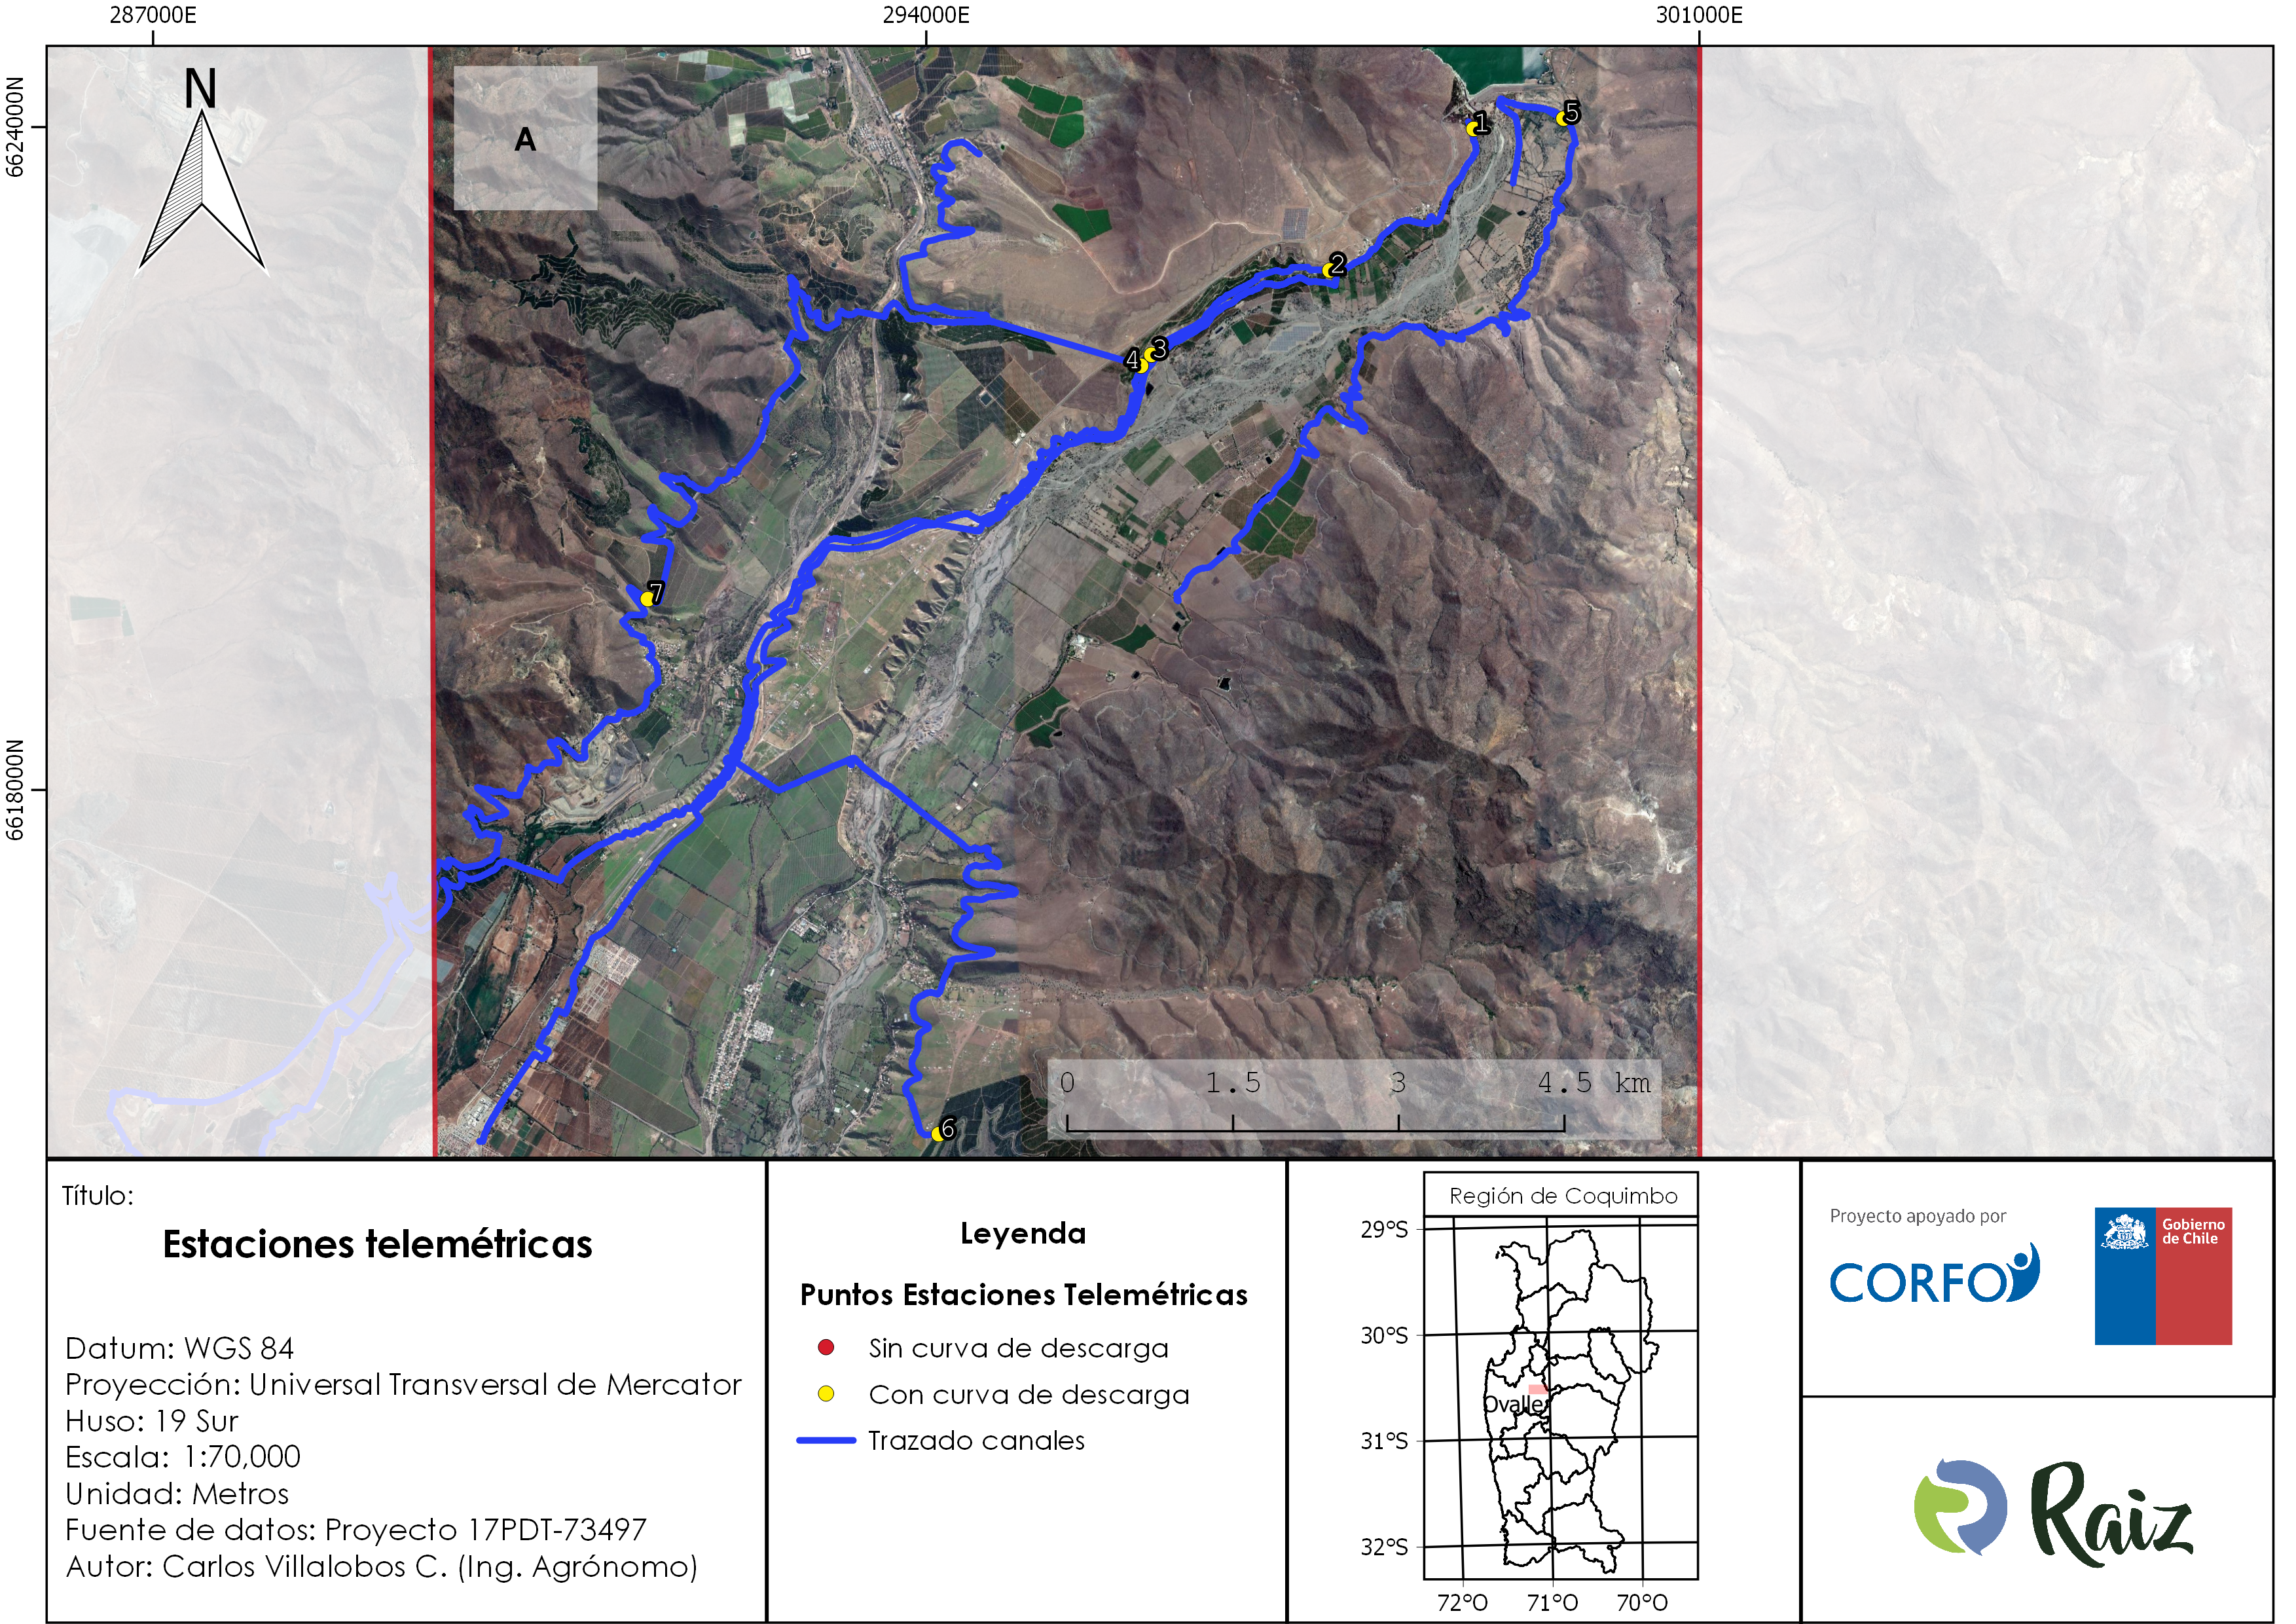
\includegraphics[width=\columnwidth, angle = 0]{./Cartografia/A.png}
   \caption{Imagen zona A, distribución de las estaciones de telemetría}
\end{sidewaysfigure}

\clearpage

\begin{sidewaysfigure}[htb]
   \centering
   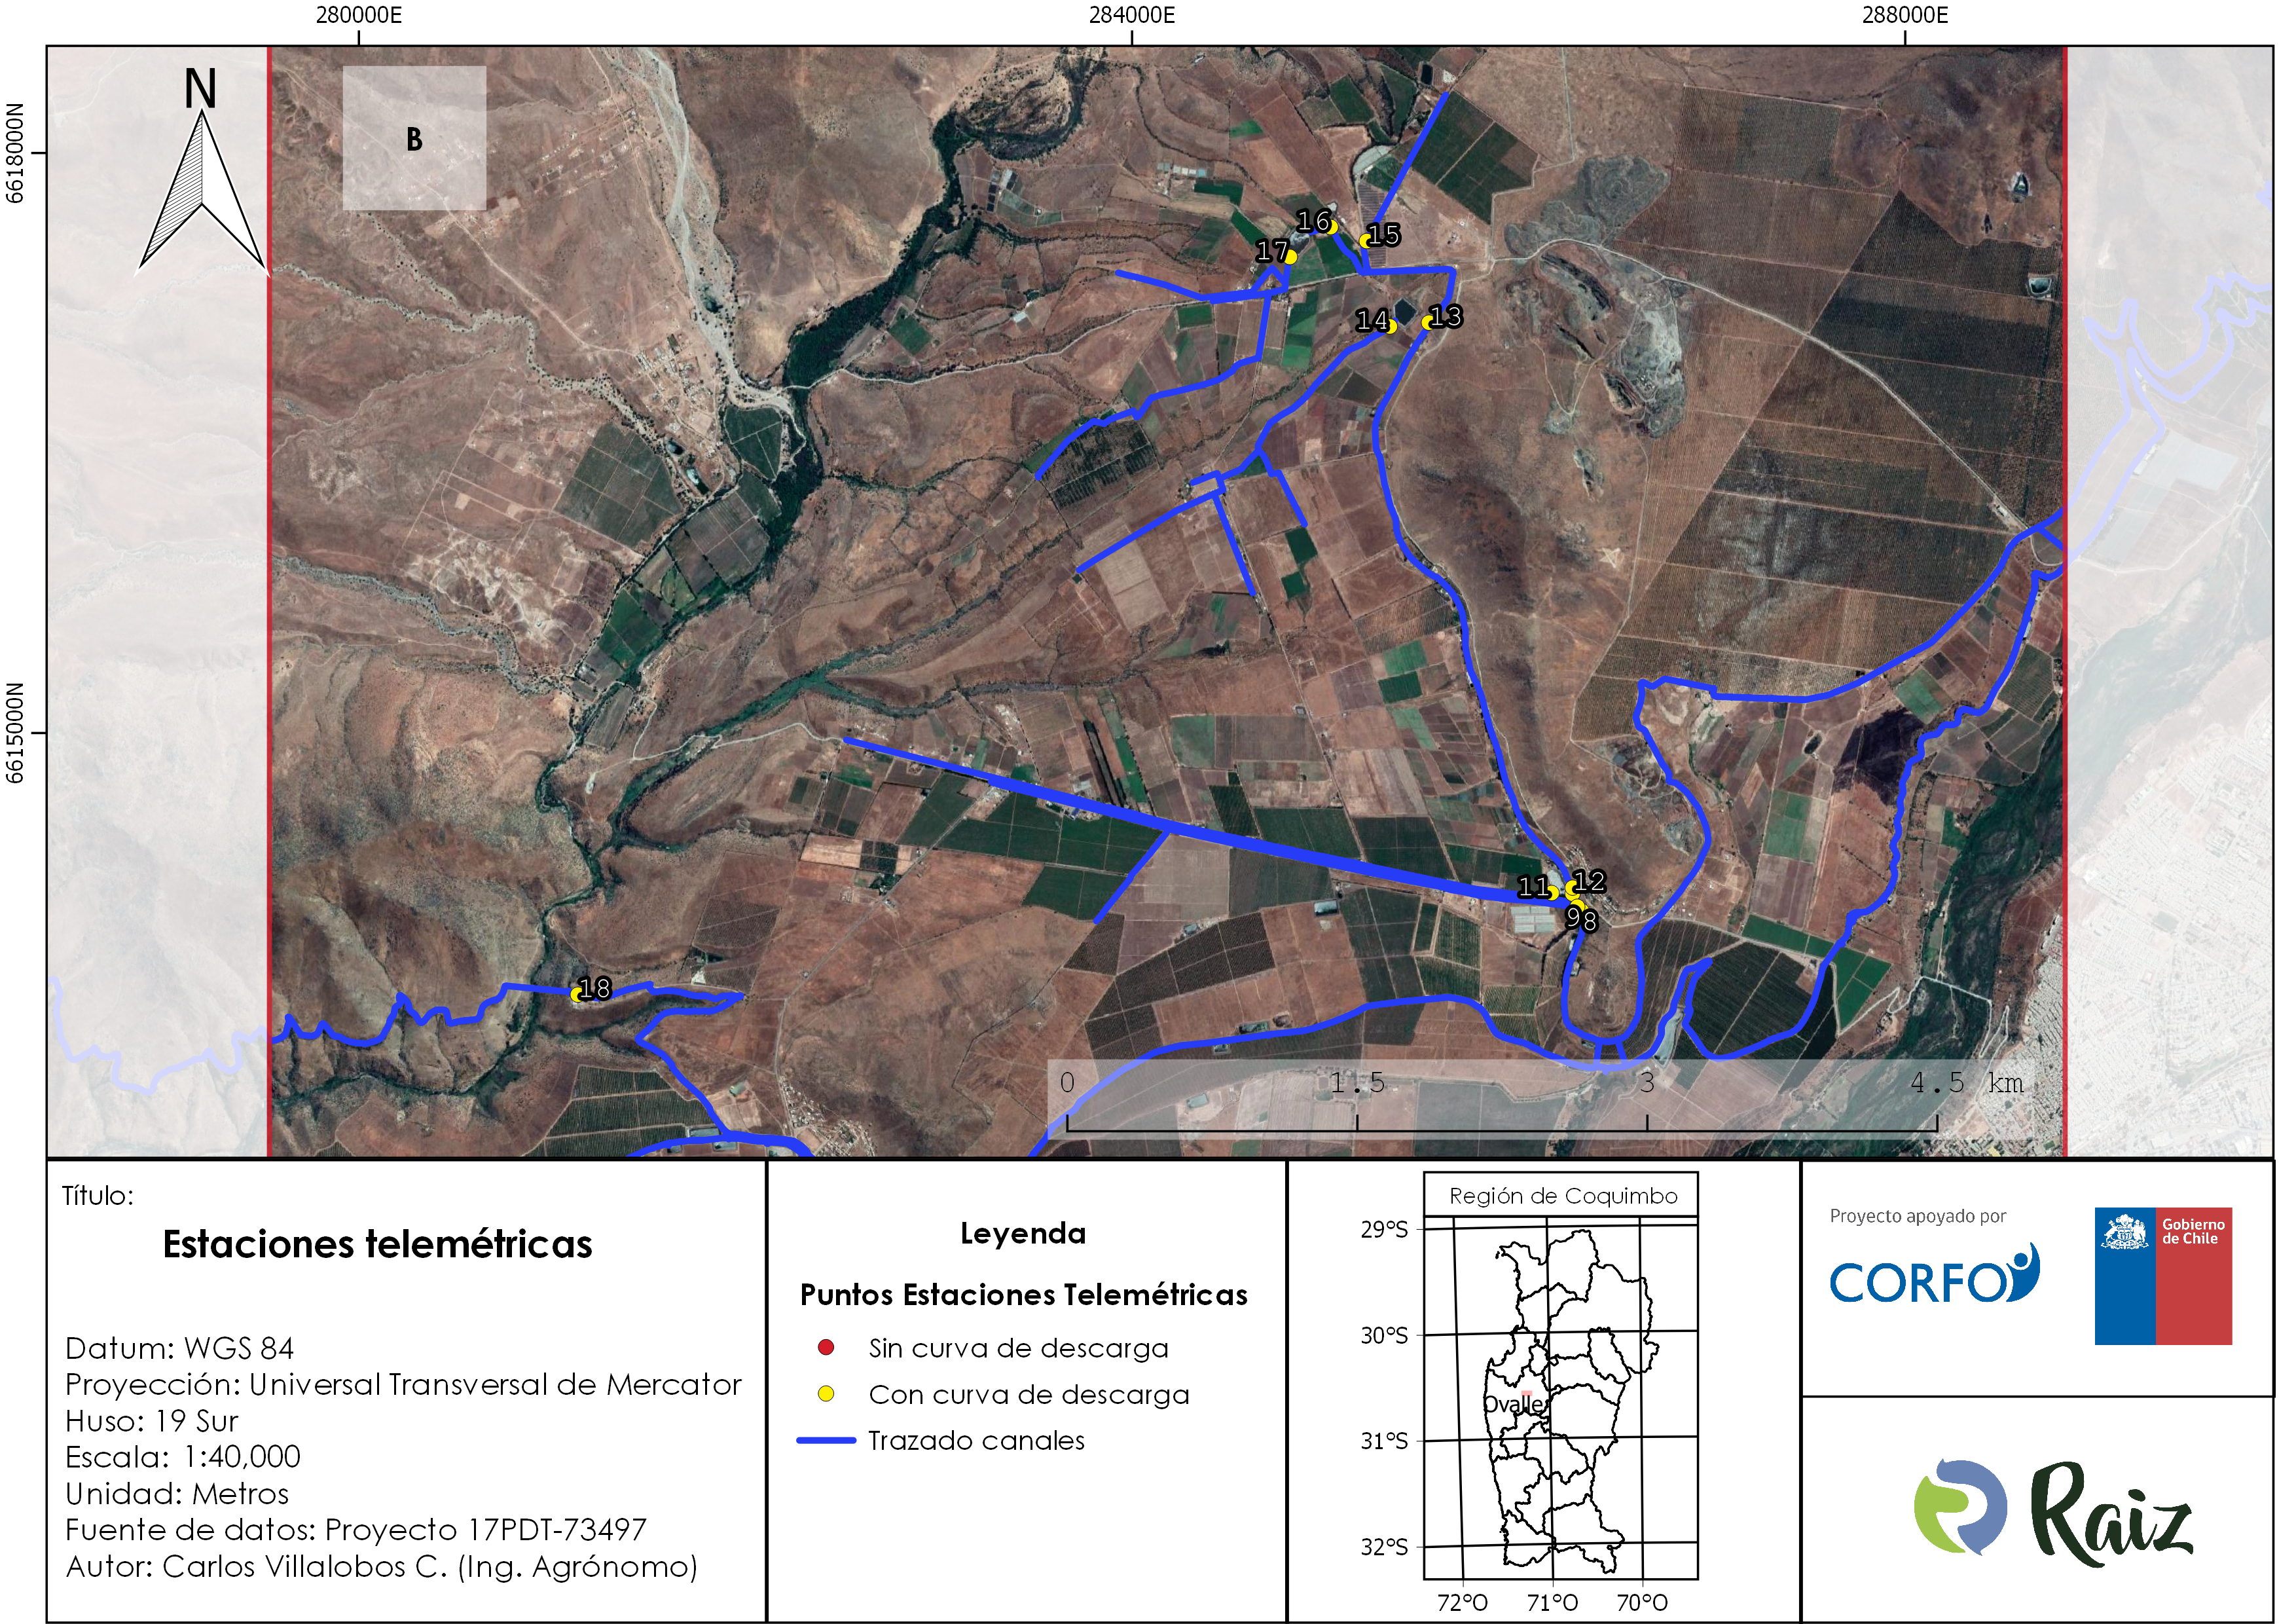
\includegraphics[width=\columnwidth, angle = 0]{./Cartografia/B.png}
   \caption{Imagen zona B, distribución de las estaciones de telemetría}
\end{sidewaysfigure}

\clearpage

\begin{sidewaysfigure}[htb]
   \centering
   \includegraphics[width=\columnwidth, angle = 0]{./Cartografia/C.png}
   \caption{Imagen zona C, distribución de las estaciones de telemetría}
\end{sidewaysfigure}

\clearpage

La información general de cada punto de monitoreo analizado, además de
sus respectivas curvas de descarga, se presentan en los siguientes
puntos, además del detalle de aforos realizados, con su desviación estándar y coeficiente de variabilidad.


\section{Estado de las curvas de descarga de las estaciones telemétricas}

La demanda de agua y disponibilidad de caudales, ha permitido realizar los aforos de las siguientes estaciones de telemetría. Donde se generaron las curvas de descarga para la mayor parte, exceptuando las que no poseen aforos en caudales críticos, falta el nivel base, no cumplen con las condiciones mínimas hidráulicas o no corresponden a una estación como tal. Las que se deben ajustar a medida que se realicen los aforos faltantes según la demanda de agua de la temporada, alcanzando un mínimo de 7 alturas de lámina de agua. El detalle de cada una es expuesto en el cuadro que se presenta a continuación:

\begin{table}[H]
 \caption{Estado de las curvas de descarga de las estaciones telemétricas}
 \centering
 \begin{tabu} {cccc}
 \toprule
 \textbf{ID} & \textbf{Estación de telemetría} & \textbf{Estado Curva} & \textbf{Alturas de agua}\\
 \midrule 
	
   1 & Matriz Recoleta - Algarrobo & Incompleta & 6\\
   2 & Matriz Tuquí Talhuén - Inicio & Completa & 7\\
   3 & Matriz Tuquí Talhuén - Fin & Completa & 7\\
   4 & Tuquí - Gato & Completa & 7\\
   5 & Villaseca - El Rincón & Completa & 7\\
   6 & Derivado Recoleta & Incompleta & 5\\
   7 & Talhuén - Munizaga & Incompleta & 6\\
   8 & Talhuén - Flor del Norte & Completa & 7\\
   9 & Colonia - Talhuén & Completa & 7\\
   10 & Embalse El Uno - Entrada & Completa & 7\\
   11 & Embalse El Uno - Salida & Completa & 7\\
   12 & Flor del Norte & Completa & 7\\
   13 & Embalse El Seis - Entrada & Completa & 7\\
   14 & Embalse El Seis - Salida & Completa & 7\\
   15 & San Luis & Incompleta & 6\\
   16 & Embalse El nueve - Entrada & Completa & 7\\
   17 & Embalse El Nueve - Salida & Incompleta & 6\\
   18 & Villalón - La Placa & Incompleta & 4\\
   19 & Villalón - Peñita Tamaya & Incompleta & 3\\
   20 & Villalón - Entrada Embalse Concepción & Completa & 7\\
   21 & Cerrillos Pobres - Peñita & Completa & 7\\
   22 & El Olivo por Alcayaga & Completa & 7\\
   23 & Cerrillos Pobres antes San Juan & Incompleta & 6\\
   24 & San Juan por los Olivos & Completa & 7\\
   25 & El Progreso & Completa & 7\\
   26 & Embalse El Progreso - Salida & Completa & 7\\
   27 & San Guillermo & Completa & 7\\
   28 & Rumiñan & Completa & 7\\
   29 & Embalse Rumiñan - Salida & Completa & 7\\
   30 & San Antonio Izquierdo & Completa & 7\\
   31 & El Romero & Completa & 7\\
   32 & El Olivo   & Completa & 7\\
   33 & Embalse Rumay - Salida & Completa & 7\\
   34 & San Guillermo colero & Incompleta & 0\\
   35 & Arquería & N/C & N/C\\
   36 & El Churque - Entrada & Completa & 8\\
   37 & Control Agrícola Tamaya & Completa & 7\\
   38 & Antes de Entrega Rumay & Incompleta & 0\\
   39 & Embalse Rumay - Entrada & Completa & 7\\
   40 & Embalse Bandurrias - Entrada & Incompleta & 0\\
   41 & Embalse Santa Cristina - Entrada & Completa & 8\\
   42 & Embalse Santa Cristina - Salida & Completa & 7\\
   
   \hline 
 \end{tabu}
\end{table}

En la sección de anexos se adjunta la tabla con el desarrollo
centimétrico de cada una de las curvas y su ficha de resumen.

\clearpage
\section{Estación telemétrica Matriz Recoleta - Algarrobo (ID:1)}

\subsection{Estación de telemetría y sección de aforo}

La estación de telemetría denominada ``Matriz Recoleta – Algarrobo'', se encuentra ubicada en el sector de Algarrobo, y es el primer punto de control de la red hídrica en la ribera derecha del río Hurtado, perteneciente a la ACER. La estación de aforo cuenta con un pozo de aquietamiento para la estabilización del flujo y así registrar la altura de lámina de agua mediante una regla limnimétrica situada en su interior, la que permite medir valores desde los 0,0 m hasta los 2,0 m. La sección de aforo se encuentra localizada a 200 m aguas abajo aproximadamente, la que no presenta pérdidas significativas según el protocolo de determinación de pérdidas por tramo, según su localización. Presenta una geometría de tipo rectangular y se encuentra revestida con hormigón, además tiene un ancho de 3,17 m y una altura de muro de 1,19 m. Se determinó realizar los aforos para la construcción de la curva de descarga en este lugar, ya que, la sección ubicada frente a la estación de aforo no reúne las condiciones mínimas establecidas por protocolo para la realización de aforos, específicamente por cambio de ancho en la sección de conducción por la presencia de entregas, lo que altera el flujo normal. La regulación de caudal para este punto de control se realiza mediante una válvula, ubicada en la salida del embalse Recoleta, a 90,0 m aproximadamente.

\begin{figure}[H]
  \centering
\begin{subfigure}{.49\textwidth}
  \includegraphics[width=\textwidth, angle = 0]{./Data/foto1_AA.jpg}
\end{subfigure}
\hfill
\begin{subfigure}{.49\textwidth}
  \includegraphics[width=\textwidth, angle = 0]{./Data/foto2_AA.jpg}
\end{subfigure}
\caption{Imágenes de la estación de telemetría y sección de aforo Matriz Recoleta - Algarrobo}
\label{fig:fotos_1}
\end{figure}

El esquema de la sección de aforo es el siguiente:

\begin{figure}[H]
  \centering
  \includegraphics[width=.9\textwidth]{temp/esquema_AA.pdf}
\caption{Esquema de la sección de aforo Matriz Recoleta - Algarrobo}
\label{fig:Esquema_AA}
\end{figure}

\subsection{Curva de descarga}\label{curva-de-descarga}

La construcción de la curva de descarga se realizó con 15 aforos, correspondientes a 5 alturas de lámina de agua, registradas en la regla limnimétrica ubicada en el interior del pozo de aquietamiento, además se adicionó una altura correspondiente al nivel base, cuyo registro fue de 0,47 m, debido al aforador de tipo vertedero presente en la sección frente a la estación de aforo, equivalente al caudal 0,0 l/s. Para la altura correspondiente al caudal máximo promedio aforado, se registró una altura de 1,20 m, equivalente a 4.203,0 l/s. Los caudales teóricos para esta estación de aforo fluctúan entre 0,0 l/s y 7.000,0 l/s, pero debido a la demanda de esta temporada, no se ha podido realizar los aforos adecuados para caudales máximos, ajustando la construcción de esta curva al caudal máximo aforado.\\
\\
Los valores de desviación estándar y coeficiente de variabilidad muestran una buena correlación estadística. En el caso de la desviación estándar, se presentan valores entre un mínimo de 0,409 y un máximo de 15,048, los que se consideran aceptados para el aforo de canales abiertos y para el caudal conducido en esta sección. Para el coeficiente de variabilidad todos los resultados obtenidos se clasifican como muy buenos, ya que son menores al 2\%, los cuales se consideran dentro del error propio del equipo de medición.

\begin{table} [H]

\caption{\label{tab:unnamed-chunk-3}Resumen de aforos estación telemétrica Matriz Recoleta - Algarrobo}
\centering
\begin{tabu} to \linewidth {>{\centering}X>{\centering}X>{\centering}X>{\centering}X>{\centering}X}
\toprule
\textbf{Altura (m)} & \textbf{Caudal (l/s)} & \textbf{Caudal promedio (l/s)} & \textbf{Desviación estándar} & \textbf{Coeficiente de variabilidad (\%)}\\
\midrule
 & 291,865 &  &  & \\

 & 291,903 &  &  & \\

\multirow{-3}{*}{\centering\arraybackslash 0,58} & 292,592 & \multirow{-3}{*}{\centering\arraybackslash 292,120} & \multirow{-3}{*}{\centering\arraybackslash 0,409} & \multirow{-3}{*}{\centering\arraybackslash 0,140}\\
\cmidrule{1-5}
 & 454,791 &  &  & \\

 & 455,476 &  &  & \\

\multirow{-3}{*}{\centering\arraybackslash 0,63} & 456,309 & \multirow{-3}{*}{\centering\arraybackslash 455,526} & \multirow{-3}{*}{\centering\arraybackslash 0,760} & \multirow{-3}{*}{\centering\arraybackslash 0,167}\\
\cmidrule{1-5}
 & 1.304,393 &  &  & \\

 & 1.316,918 &  &  & \\

\multirow{-3}{*}{\centering\arraybackslash 0,80} & 1.334,356 & \multirow{-3}{*}{\centering\arraybackslash 1.318,556} & \multirow{-3}{*}{\centering\arraybackslash 15,048} & \multirow{-3}{*}{\centering\arraybackslash 1,141}\\
\cmidrule{1-5}
 & 1.848,775 &  &  & \\

 & 1.860,748 &  &  & \\

\multirow{-3}{*}{\centering\arraybackslash 0,87} & 1.861,370 & \multirow{-3}{*}{\centering\arraybackslash 1.856,964} & \multirow{-3}{*}{\centering\arraybackslash 7,099} & \multirow{-3}{*}{\centering\arraybackslash 0,382}\\
\cmidrule{1-5}
 & 4.193,093 &  &  & \\

 & 4.201,600 &  &  & \\

\multirow{-3}{*}{\centering\arraybackslash 1,20} & 4.214,446 & \multirow{-3}{*}{\centering\arraybackslash 4.203,046} & \multirow{-3}{*}{\centering\arraybackslash 10,750} & \multirow{-3}{*}{\centering\arraybackslash 0,256}\\
\bottomrule
\end{tabu}
\end{table}

Ecuación de descarga de caudal:

\[Q = 6587,15*(h_w - h_0)^{1,42}\]

donde:

\(Q\) = Caudal (l/s); \(h_w\) = altura de referencia (m); \(h_0\) =
peralte (m).

El coeficiente \(R^2\): 0,999

\begin{figure}[H]
  \centering
  \includegraphics[width=.9\textwidth]{temp/curva_AA.pdf}
\caption{Curva de descarga de la estación de telemetría Matriz Recoleta - Algarrobo}
\label{fig:Curva_AA}
\end{figure}

\clearpage
\section{Estación telemétrica Matriz Tuquí Talhuén - Inicio (ID:2)}

\subsection{Estación de telemetría y sección de aforo}

El punto de control denominado ``Matriz Tuquí Talhuén – Inicio'', se encuentra ubicado en el sector de Algarrobo. La sección de aforo se ubica frente a la estación de medición del canal y es de forma rectangular, encontrándose revestida con hormigón. El ancho de la sección es de 1,70 m y sus muros alcanzan una altura de 1,50 m, además presenta un aforador de tipo vertedero. La estación de aforo cuenta con un pozo de aquietamiento con limnímetro, que permite registrar valores entre los 0,0 m y 1,54 m. La regulación de caudal en este punto de control se realiza mediante una compuerta, la que se encuentra ubicada a 75,0 m aproximadamente.

\begin{figure}[H]
  \centering
\begin{subfigure}{.49\textwidth}
  \includegraphics[width=\textwidth, angle = 180]{./Data/foto1_AB.JPG}
\end{subfigure}
\hfill
\begin{subfigure}{.49\textwidth}
  \includegraphics[width=\textwidth, angle = 0]{./Data/foto2_AB.JPG}
\end{subfigure}
\caption{Imágenes de la estación de telemetría y sección de aforo Matriz Tuquí Talhuén - Inicio}
\label{fig:fotos_2}
\end{figure}

El esquema de la sección de aforo es el siguiente:

\begin{figure}[H]
  \centering
  \includegraphics[width=.9\textwidth]{temp/esquema_AB.pdf}
\caption{Esquema de la sección de aforo Matriz Tuquí Talhuén - Inicio}
\label{fig:Esquema_AB}
\end{figure}

\subsection{Curva de descarga}\label{curva-de-descarga-1}

Su curva de descarga se construyó con 18 aforos, equivalentes a 6 alturas de lámina de agua, más una altura para el nivel base, equivalente a 0,0 l/s, las que fueron registradas en la regla limnimétrica que se observa al interior del pozo de aquietamiento. Las alturas de lámina de agua que componen la curva de descarga varían entre los 0,27 m para caudal 0,0 l/s y 0,86 m para el caudal máximo aforado de 1.810,49 l/s. Estos caudales obtenidos se encuentran en los rangos esperados de los caudales teóricos de esta estación de aforo, los que oscilan entre 0,0 l/s y 2.000,0 l/s.\\
\\
Los valores de desviación estándar se encuentran en un rango de 2,488 y 7,495, los cuales representan una correcta dispersión de datos para caudales de esta magnitud, y aceptados para aforos de canales abiertos. Para el coeficiente de variabilidad todos los resultados obtenidos se clasifican como muy buenos, ya que son menores al 2\%, los que se pueden atribuir al error propio del equipo de medición.

\begin{table}[H]

\caption{\label{tab:unnamed-chunk-3}Resumen de aforos estación telemétrica Matriz Tuquí Talhuén - Inicio}
\centering
\begin{tabu} to \linewidth {>{\centering}X>{\centering}X>{\centering}X>{\centering}X>{\centering}X}
\toprule
\textbf{Altura (m)} & \textbf{Caudal (l/s)} & \textbf{Caudal promedio (l/s)} & \textbf{Desviación estándar} & \textbf{Coeficiente de variabilidad (\%)}\\
\midrule
 & 285,292 &  &  & \\

 & 287,730 &  &  & \\

\multirow{-3}{*}{\centering\arraybackslash 0,47} & 290,269 & \multirow{-3}{*}{\centering\arraybackslash 287,764} & \multirow{-3}{*}{\centering\arraybackslash 2,488} & \multirow{-3}{*}{\centering\arraybackslash 0,865}\\
\cmidrule{1-5}
 & 517,162 &  &  & \\

 & 521,750 &  &  & \\

\multirow{-3}{*}{\centering\arraybackslash 0,55} & 522,074 & \multirow{-3}{*}{\centering\arraybackslash 520,329} & \multirow{-3}{*}{\centering\arraybackslash 2,747} & \multirow{-3}{*}{\centering\arraybackslash 0,528}\\
\cmidrule{1-5}
 & 986,734 &  &  & \\

 & 989,412 &  &  & \\

\multirow{-3}{*}{\centering\arraybackslash 0,67} & 992,043 & \multirow{-3}{*}{\centering\arraybackslash 989,396} & \multirow{-3}{*}{\centering\arraybackslash 2,654} & \multirow{-3}{*}{\centering\arraybackslash 0,268}\\
\cmidrule{1-5}
 & 1.209,098 &  &  & \\

 & 1.211,270 &  &  & \\

\multirow{-3}{*}{\centering\arraybackslash 0,73} & 1.223,029 & \multirow{-3}{*}{\centering\arraybackslash 1.214,466} & \multirow{-3}{*}{\centering\arraybackslash 7,495} & \multirow{-3}{*}{\centering\arraybackslash 0,617}\\
\cmidrule{1-5}
 & 1.628,290 &  &  & \\

 & 1.633,123 &  &  & \\

\multirow{-3}{*}{\centering\arraybackslash 0,82} & 1.641,079 & \multirow{-3}{*}{\centering\arraybackslash 1.634,164} & \multirow{-3}{*}{\centering\arraybackslash 6,458} & \multirow{-3}{*}{\centering\arraybackslash 0,395}\\
\cmidrule{1-5}
 & 1.807,154 &  &  & \\

 & 1.807,298 &  &  & \\

\multirow{-3}{*}{\centering\arraybackslash 0,86} & 1.817,023 & \multirow{-3}{*}{\centering\arraybackslash 1.810,491} & \multirow{-3}{*}{\centering\arraybackslash 5,657} & \multirow{-3}{*}{\centering\arraybackslash 0,312}\\
\bottomrule
\end{tabu}
\end{table}

Ecuación de descarga de caudal:

\[Q = 4358,75*(h_w - h_0)^{1,65}\]

donde:

\(Q\) = Caudal (l/s); \(h_w\) = altura de referencia (m); \(h_0\) =
peralte (m).

El coeficiente \(R^2\): 0,999

\begin{figure}[H]
  \centering
  \includegraphics[width=.9\textwidth]{temp/curva_AB.pdf}
\caption{Curva de descarga de la estación de telemetría Matriz Tuquí Talhuén - Inicio}
\label{fig:Curva_AB}
\end{figure}

\clearpage
\section{Estación telemétrica Matriz Tuquí Talhuén - Fin (ID:3)}

\subsection{Estación de telemetría y sección de aforo}

El punto de control denominado ``Matriz Tuquí Talhuén – Fin'', se localiza en el interior de la agrícola ``La Chapeana''. La sección de aforo se ubica aproximadamente a 100 m. aguas arriba de la estación de monitoreo, debido a que el canal se encuentra revestido con un embovedado de hormigón, y en este sector posee un acceso habilitado especialmente para realización de aforos a través de puertas metálicas. Su geometría es de tipo rectangular, con un ancho de 1,70 m, altura de muro de 1,66 m y no posee aforador. El pozo de aquietamiento de la estación de aforo puede registrar alturas de lámina de agua, a través de un limnímetro, desde los 0,0 m hasta los 1,30 m. Este punto de control no tiene regulación de caudal, por lo que depende del caudal entregado en el inicio del canal Matriz Tuquí Talhuén y de las entregas presentes en el trazado.

\begin{figure}[H]
  \centering
\begin{subfigure}{.49\textwidth}
  \includegraphics[width=\textwidth, angle = 0]{./Data/foto1_AC.JPG}
\end{subfigure}
\hfill
\begin{subfigure}{.49\textwidth}
  \includegraphics[width=\textwidth, angle = 0]{./Data/foto2_AC.JPG}
\end{subfigure}
\caption{Imágenes de la estación de telemetría y sección de aforo Matriz Tuquí Talhuén - Fin}
\label{fig:fotos_3}
\end{figure}

El esquema de la sección de aforo es el siguiente:

\begin{figure}[H]
  \centering
  \includegraphics[width=.9\textwidth]{temp/esquema_AC.pdf}
\caption{Esquema de la sección de aforo Matriz Tuquí Talhuén - Fin}
\label{fig:Esquema_AC}
\end{figure}

\subsection{Curva de descarga}\label{curva-de-descarga-2}

Esta curva de descarga contiene 18 aforos, los que equivalen a 6 alturas de lámina de agua, más una altura para el nivel base, equivalente a 0,0 l/s, que fueron registradas con la regla limnimétrica del interior del pozo de aquietamiento. La regla limnimétrica varía entre un mínimo de 0,0 m. y máximo de 1,52 m, registrando para el caudal 0,0 l/s un análogo del valor mínimo y para 1.724,68 l/s de caudal máximo promedio aforado una altura de 0,68 m. Estos caudales aforados se desempeñan dentro del 86\% de los caudales teóricos, que corresponden a valores entre 0,0 l/s y 2000,0 l/s.\\
\\
Los valores de desviación estándar y coeficiente de variabilidad muestran una buena correlación estadística. Para la desviación estándar, se presentan valores de dispersión bajo 4,733, exceptuando el caso de la altura de lámina de agua de 0,64 m, encontrándose valores de 18,919, los que son aceptados y considerados como buenos de acuerdo a la magnitud de los caudales aforados. Para el coeficiente de variabilidad todos los resultados obtenidos se clasifican como muy buenos, ya que son menores al 2\%, aplicable al error propio del equipo de medición.

\begin{table}[H]

\caption{\label{tab:unnamed-chunk-3}Resumen de aforos estación telemétrica Matriz Tuquí Talhuén - Fin}
\centering
\begin{tabu} to \linewidth {>{\centering}X>{\centering}X>{\centering}X>{\centering}X>{\centering}X}
\toprule
\textbf{Altura (m)} & \textbf{Caudal (l/s)} & \textbf{Caudal promedio (l/s)} & \textbf{Desviación estándar} & \textbf{Coeficiente de variabilidad (\%)}\\
\midrule
 & 275,912 &  &  & \\

 & 278,260 &  &  & \\

\multirow{-3}{*}{\centering\arraybackslash 0,22} & 279,732 & \multirow{-3}{*}{\centering\arraybackslash 277,968} & \multirow{-3}{*}{\centering\arraybackslash 1,927} & \multirow{-3}{*}{\centering\arraybackslash 0,693}\\
\cmidrule{1-5}
 & 540,100 &  &  & \\

 & 543,144 &  &  & \\

\multirow{-3}{*}{\centering\arraybackslash 0,33} & 549,382 & \multirow{-3}{*}{\centering\arraybackslash 544,209} & \multirow{-3}{*}{\centering\arraybackslash 4,732} & \multirow{-3}{*}{\centering\arraybackslash 0,870}\\
\cmidrule{1-5}
 & 959,692 &  &  & \\

 & 962,402 &  &  & \\

\multirow{-3}{*}{\centering\arraybackslash 0,47} & 963,216 & \multirow{-3}{*}{\centering\arraybackslash 961,770} & \multirow{-3}{*}{\centering\arraybackslash 1,845} & \multirow{-3}{*}{\centering\arraybackslash 0,192}\\
\cmidrule{1-5}
 & 1.103,315 &  &  & \\

 & 1.108,317 &  &  & \\

\multirow{-3}{*}{\centering\arraybackslash 0,56} & 1.112,739 & \multirow{-3}{*}{\centering\arraybackslash 1.108,124} & \multirow{-3}{*}{\centering\arraybackslash 4,715} & \multirow{-3}{*}{\centering\arraybackslash 0,425}\\
\cmidrule{1-5}
 & 1.563,279 &  &  & \\

 & 1.573,286 &  &  & \\

\multirow{-3}{*}{\centering\arraybackslash 0,64} & 1.599,885 & \multirow{-3}{*}{\centering\arraybackslash 1.578,817} & \multirow{-3}{*}{\centering\arraybackslash 18,919} & \multirow{-3}{*}{\centering\arraybackslash 1,198}\\
\cmidrule{1-5}
 & 1.721,471 &  &  & \\

 & 1.724,321 &  &  & \\

\multirow{-3}{*}{\centering\arraybackslash 0,68} & 1.728,259 & \multirow{-3}{*}{\centering\arraybackslash 1.724,684} & \multirow{-3}{*}{\centering\arraybackslash 3,408} & \multirow{-3}{*}{\centering\arraybackslash 0,198}\\
\bottomrule
\end{tabu}
\end{table}

Ecuación de descarga de caudal:

\[Q = 693,19* h_w + 2672,87*{{h_w}^2}\]

donde:

\(Q\) = Caudal (l/s); \(h_w\) = altura de referencia (m).

El coeficiente \(R^2\): 0,988

\begin{figure}[H]
  \centering
  \includegraphics[width=.9\textwidth]{temp/curva_AC.pdf}
\caption{Curva de descarga de la estación de telemetría Matriz Tuquí Talhuén - Fin}
\label{fig:Curva_AC}
\end{figure}

\clearpage
\section{Estación telemétrica Tuquí - Gato (ID:4)}

\subsection{Estación de telemetría y sección de aforo}

La estación de telemetría denominada ``Tuquí – Gato'', se ubica en el interior de la Agrícola ``La Chapeana'', y corresponde al inicio del Canal Tuquí. La sección de aforo se ubica a 4,65 m aguas abajo de la estación, debido a un cambio de ancho en la sección de conducción frente a la estación. Posee forma geométrica rectangular, encontrándose revestida con hormigón roca, además, tiene un ancho de 2,43 m, altura de muro de 1,235 m y presenta un aforador de tipo vertedero ubicado a 48,20 m aguas abajo de la estación. El limnímetro del pozo de aquietamiento permite medir alturas de lámina de agua entre los 0,0 m y los 1,30 m. La regulación de este punto de control se realiza mediante una compuerta ubicada a 20,0 m.

\begin{figure}[H]
  \centering
\begin{subfigure}{.49\textwidth}
  \includegraphics[width=\textwidth, angle = 0]{./Data/foto1_AD.jpg}
\end{subfigure}
\hfill
\begin{subfigure}{.49\textwidth}
  \includegraphics[width=\textwidth, angle = 180]{./Data/foto2_AD.JPG}
\end{subfigure}
\caption{Imágenes de la estación de telemetría y sección de aforo Tuquí - Gato}
\label{fig:fotos_4}
\end{figure}

El esquema de la sección de aforo es el siguiente:

\begin{figure}[H]
  \centering
  \includegraphics[width=.9\textwidth]{temp/esquema_AD.pdf}
\caption{Esquema de la sección de aforo Tuquí - Gato}
\label{fig:Esquema_AD}
\end{figure}

\subsection{Curva de descarga}\label{curva-de-descarga-3}

La curva de descarga se generó a partir de 7 alturas de lámina de agua, registradas en el limnímetro del pozo de aquietamiento y que corresponden a 18 aforos, más la altura de nivel base. La altura de nivel base, correspondiente al caudal 0,0 l/s, es de 0,30 m, debido al aforador de tipo vertedero que posee. El caudal máximo promedio aforado es de 482,59 l/s, equivalente a 0,575 m. Los caudales teóricos para esta estación de aforo corresponden a valores entre los 0,0 l/s y 450,0 l/s, siendo el máximo promedio aforado mayor en 32,59 l/s.\\
\\
Los valores de desviación estándar son de magnitud baja, valores menores a 3,838, debido principalmente a que el flujo es muy estable. Los valores del coeficiente de variabilidad de la mayoría de las alturas de lámina de agua se presentan bajo 2\%, es decir, como muy buenos, exceptuando el valor de los aforos para caudal mínimo, el cual presenta un valor de 2,576\%, considerado como bueno. 

\begin{table}[H]

\caption{\label{tab:unnamed-chunk-3}Resumen de aforos estación telemétrica Tuquí - Gato}
\centering
\begin{tabu} to \linewidth {>{\centering}X>{\centering}X>{\centering}X>{\centering}X>{\centering}X}
\toprule
\textbf{Altura (m)} & \textbf{Caudal (l/s)} & \textbf{Caudal promedio (l/s)} & \textbf{Desviación estándar} & \textbf{Coeficiente de variabilidad (\%)}\\
\midrule
 & 89,251 &  &  & \\

 & 89,460 &  &  & \\

\multirow{-3}{*}{\centering\arraybackslash 0,395} & 93,399 & \multirow{-3}{*}{\centering\arraybackslash 90,703} & \multirow{-3}{*}{\centering\arraybackslash 2,337} & \multirow{-3}{*}{\centering\arraybackslash 2,576}\\
\cmidrule{1-5}
 & 165,677 &  &  & \\

 & 167,274 &  &  & \\

\multirow{-3}{*}{\centering\arraybackslash 0,440} & 167,690 & \multirow{-3}{*}{\centering\arraybackslash 166,880} & \multirow{-3}{*}{\centering\arraybackslash 1,063} & \multirow{-3}{*}{\centering\arraybackslash 0,637}\\
\cmidrule{1-5}
 & 227,618 &  &  & \\

 & 229,944 &  &  & \\

\multirow{-3}{*}{\centering\arraybackslash 0,470} & 231,014 & \multirow{-3}{*}{\centering\arraybackslash 229,525} & \multirow{-3}{*}{\centering\arraybackslash 1,736} & \multirow{-3}{*}{\centering\arraybackslash 0,756}\\
\cmidrule{1-5}
 & 271,672 &  &  & \\

 & 274,975 &  &  & \\

\multirow{-3}{*}{\centering\arraybackslash 0,490} & 275,415 & \multirow{-3}{*}{\centering\arraybackslash 274,021} & \multirow{-3}{*}{\centering\arraybackslash 2,046} & \multirow{-3}{*}{\centering\arraybackslash 0,747}\\
\cmidrule{1-5}
 & 382,619 &  &  & \\

 & 383,036 &  &  & \\

\multirow{-3}{*}{\centering\arraybackslash 0,540} & 385,679 & \multirow{-3}{*}{\centering\arraybackslash 383,778} & \multirow{-3}{*}{\centering\arraybackslash 1,659} & \multirow{-3}{*}{\centering\arraybackslash 0,432}\\
\cmidrule{1-5}
 & 478,252 &  &  & \\

 & 483,962 &  &  & \\

\multirow{-3}{*}{\centering\arraybackslash 0,575} & 485,549 & \multirow{-3}{*}{\centering\arraybackslash 482,588} & \multirow{-3}{*}{\centering\arraybackslash 3,838} & \multirow{-3}{*}{\centering\arraybackslash 0,795}\\
\bottomrule
\end{tabu}
\end{table}

Ecuación de descarga de caudal:

\[Q = 3574,72*(h_w - h_0)^{1,55}\]

donde:

\(Q\) = Caudal (l/s); \(h_w\) = altura de referencia (m); \(h_0\) =
peralte (m).

El coeficiente \(R^2\): 1

\begin{figure}[H]
  \centering
  \includegraphics[width=.9\textwidth]{temp/curva_AD.pdf}
\caption{Curva de descarga de la estación de telemetría Tuquí - Gato}
\label{fig:Curva_AD}
\end{figure}

\clearpage
\section{Estación telemétrica Villaseca - El Rincón (ID:5)}

\subsection{Estación de telemetría y sección de aforo}

La estación de telemetría denominada ``Villaseca – El Rincón'', se encuentra ubicada en el sector llamado El Rincón, en la ribera izquierda del río Hurtado, aguas abajo del muro del embalse Recoleta. Tiene una sección de aforo de geometría tipo rectangular frente a la estación, revestida con hormigón y con acceso a través de placas de metal, ya que este sector del trazado del canal se encuentra embovedado. Posee un ancho de 1,10 m, una altura de muro de 1,28 m y no se observa ningún tipo de aforador. La regla limnimétrica del pozo de aquietamiento puede registrar valores desde los 0,0 m hasta los 1,54 m. Además debemos indicar que existe un limnímetro en la sección de aforo, el cual no se utilizó para el registro de datos. La regulación de este punto de control se realiza mediante una válvula, la que se encuentra ubicada a 600,0 m aproximadamente.


\begin{figure}[H]
  \centering
\begin{subfigure}{.49\textwidth}
  \includegraphics[width=\textwidth, angle = 0]{./Data/foto1_AE.jpg}
\end{subfigure}
\hfill
\begin{subfigure}{.49\textwidth}
  \includegraphics[width=\textwidth, angle = 0]{./Data/foto2_AE.JPG}
\end{subfigure}
\caption{Imágenes de la estación de telemetría y sección de aforo Villaseca - El Rincón}
\label{fig:fotos_5}
\end{figure}

El esquema de la sección de aforo es el siguiente:

\begin{figure}[H]
  \centering
  \includegraphics[width=.9\textwidth]{temp/esquema_AE.pdf}
\caption{Esquema de la sección de aforo Villaseca - El Rincón}
\label{fig:Esquema_AE}
\end{figure}

\subsection{Curva de descarga}\label{curva-de-descarga-4}

La curva de descarga de la estación de aforo se compone de 7 alturas de lámina de agua, obtenidas desde el nivel base, más 18 aforos. La altura mínima de lámina de agua de registro en el limnímetro del pozo de aquietamiento o nivel base, es de 0,0 m, y corresponde a un caudal de 0,0 l/s, mientras que el caudal máximo promedio aforado es de 394,59 l/s, correspondientes a 0,45 m. Los caudales teóricos de este punto de control fluctúan entre los 0,0 l/s y los 450,0 l/s, por lo que la curva de descarga se ajusta a los caudales esperados en un rango de 90\%.\\
\\
Los valores de desviación estándar son de magnitud baja, debido principalmente a que el flujo se presenta estable. Los valores del coeficiente de variabilidad se presentan bajo un 2\%, es decir como muy buenos, incluso menores a un 1\%, expresando la gran uniformidad de los datos obtenidos. 

\begin{table}[H]

\caption{\label{tab:unnamed-chunk-3}Resumen de aforos estación telemétrica Villaseca - El Rincón}
\centering
\begin{tabu} to \linewidth {>{\centering}X>{\centering}X>{\centering}X>{\centering}X>{\centering}X}
\toprule
\textbf{Altura (m)} & \textbf{Caudal (l/s)} & \textbf{Caudal promedio (l/s)} & \textbf{Desviación estándar} & \textbf{Coeficiente de variabilidad (\%)}\\
\midrule
 & 114,798 &  &  & \\

 & 114,872 &  &  & \\

\multirow{-3}{*}{\centering\arraybackslash 0,18} & 116,306 & \multirow{-3}{*}{\centering\arraybackslash 115,326} & \multirow{-3}{*}{\centering\arraybackslash 0,850} & \multirow{-3}{*}{\centering\arraybackslash 0,737}\\
\cmidrule{1-5}
 & 176,824 &  &  & \\

 & 177,171 &  &  & \\

\multirow{-3}{*}{\centering\arraybackslash 0,25} & 177,409 & \multirow{-3}{*}{\centering\arraybackslash 177,135} & \multirow{-3}{*}{\centering\arraybackslash 0,294} & \multirow{-3}{*}{\centering\arraybackslash 0,166}\\
\cmidrule{1-5}
 & 227,791 &  &  & \\

 & 228,060 &  &  & \\

\multirow{-3}{*}{\centering\arraybackslash 0,32} & 230,208 & \multirow{-3}{*}{\centering\arraybackslash 228,686} & \multirow{-3}{*}{\centering\arraybackslash 1,325} & \multirow{-3}{*}{\centering\arraybackslash 0,579}\\
\cmidrule{1-5}
 & 258,660 &  &  & \\

 & 260,135 &  &  & \\

\multirow{-3}{*}{\centering\arraybackslash 0,34} & 261,081 & \multirow{-3}{*}{\centering\arraybackslash 259,959} & \multirow{-3}{*}{\centering\arraybackslash 1,220} & \multirow{-3}{*}{\centering\arraybackslash 0,469}\\
\cmidrule{1-5}
 & 325,978 &  &  & \\

 & 327,198 &  &  & \\

\multirow{-3}{*}{\centering\arraybackslash 0,40} & 331,863 & \multirow{-3}{*}{\centering\arraybackslash 328,346} & \multirow{-3}{*}{\centering\arraybackslash 3,106} & \multirow{-3}{*}{\centering\arraybackslash 0,946}\\
\cmidrule{1-5}
 & 392,654 &  &  & \\

 & 394,567 &  &  & \\

\multirow{-3}{*}{\centering\arraybackslash 0,45} & 396,558 & \multirow{-3}{*}{\centering\arraybackslash 394,593} & \multirow{-3}{*}{\centering\arraybackslash 1,952} & \multirow{-3}{*}{\centering\arraybackslash 0,495}\\
\bottomrule
\end{tabu}
\end{table}

Ecuación de descarga de caudal:

\[Q = 453,69* h_w + 921,32*{{h_w}^2}\]

donde:

\(Q\) = Caudal (l/s); \(h_w\) = altura de referencia (m).

El coeficiente \(R^2\): 0,996

\begin{figure}[H]
  \centering
  \includegraphics[width=.9\textwidth]{temp/curva_AE.pdf}
\caption{Curva de descarga de la estación de telemetría Villaseca - El Rincón}
\label{fig:Curva_AE}
\end{figure}

\clearpage
\section{Estación telemétrica Derivado Recoleta (ID:6)}

\subsection{Estación de telemetría y sección de aforo}

La estación de telemetría denominada ``Derivado Recoleta'', se ubica en el interior de la Agrícola ``Norte'', en el sector llamado Puntilla de Barrancas. Este punto de control se localiza en el inicio del trazado del canal Derivado Recoleta y su sección de aforo se ubica frente a la estación. La sección de aforo tiene forma rectangular y esta revestida con hormigón, posee un ancho de 1,48 m y una altura de muro de 2,24 m, además posee un aforador de tipo escurrimiento crítico aguas abajo de la estación, a 4,37 m. La selección de esta sección de aforo se basó en la factibilidad técnica para la realización de los aforos. Se registró la altura de agua en el limnímetro del pozo de aquietamiento que tiene escala centimétrica,  adecuada para registrar valores entre los 0,0 m y 1,60 m, donde además se puede observar una escala con graduación volumétrica. La regulación de este punto de control se realiza mediante una compuerta ubicada a 53,20 m aproximadamente.

\begin{figure}[H]
  \centering
\begin{subfigure}{.49\textwidth}
  \includegraphics[width=\textwidth, angle = 0]{./Data/foto1_AF.jpg}
\end{subfigure}
\hfill
\begin{subfigure}{.49\textwidth}
  \includegraphics[width=\textwidth, angle = 0]{./Data/foto2_AF.jpg}
\end{subfigure}
\caption{Imágenes de la estación de telemetría y sección de aforo Derivado Recoleta}
\label{fig:fotos_6}
\end{figure}

El esquema de la sección de aforo es el siguiente:

\begin{figure}[H]
  \centering
  \includegraphics[width=.9\textwidth]{temp/esquema_AF.pdf}
\caption{Esquema de la sección de aforo Derivado Recoleta}
\label{fig:Esquema_AF}
\end{figure}

\subsection{Curva de descarga}\label{curva-de-descarga-5}

Se realizaron 12 aforos, correspondientes a 4 alturas de lámina de agua, y se adicionó la altura de nivel base para la construcción de la curva de descarga. La altura de nivel base es de 0,53 m, y corresponde a la altura mínima registrada, con un caudal de 0,0 l/s, mientras que la altura máxima promedio aforada fue de 1,47 m, equivalente una caudal promedio de 2.915,22 l/s. La curva de descarga está condicionada a los caudales disponibles durante la campaña de aforos. Los caudales teóricos de la estación de aforo varían entre los 0,0 l/s y los 3.000,0 l/s, por lo que se ajusta de buena manera al caudal máximo aforado.\\
\\
Los valores de desviación estándar son bajos, de acuerdo a la magnitud de los caudales, por lo cual tienen un alto grado de exactitud. Los valores del coeficiente de variabilidad se presentan bajo un 2\%, es decir como muy buenos, incluso menores a un 1\%, expresando la gran uniformidad de los datos obtenidos.

\begin{table}[H]

\caption{\label{tab:unnamed-chunk-3}Resumen de aforos estación telemétrica Derivado Recoleta}
\centering
\begin{tabu} to \linewidth {>{\centering}X>{\centering}X>{\centering}X>{\centering}X>{\centering}X}
\toprule
\textbf{Altura (m)} & \textbf{Caudal (l/s)} & \textbf{Caudal promedio (l/s)} & \textbf{Desviación estándar} & \textbf{Coeficiente de variabilidad (\%)}\\
\midrule
 & 1.470,27 &  &  & \\

 & 1.478,70 &  &  & \\

\multirow{-3}{*}{\centering\arraybackslash 1,140} & 1.485,62 & \multirow{-3}{*}{\centering\arraybackslash 1.478,19} & \multirow{-3}{*}{\centering\arraybackslash 7,690} & \multirow{-3}{*}{\centering\arraybackslash 0,520}\\
\cmidrule{1-5}
 & 1.871,06 &  &  & \\

 & 1.876,24 &  &  & \\

\multirow{-3}{*}{\centering\arraybackslash 1,235} & 1.876,31 & \multirow{-3}{*}{\centering\arraybackslash 1.874,53} & \multirow{-3}{*}{\centering\arraybackslash 3,010} & \multirow{-3}{*}{\centering\arraybackslash 0,161}\\
\cmidrule{1-5}
 & 2.550,28 &  &  & \\

 & 2.577,72 &  &  & \\

\multirow{-3}{*}{\centering\arraybackslash 1,400} & 2.589,35 & \multirow{-3}{*}{\centering\arraybackslash 2.572,45} & \multirow{-3}{*}{\centering\arraybackslash 20,062} & \multirow{-3}{*}{\centering\arraybackslash 0,780}\\
\cmidrule{1-5}
 & 2.896,46 &  &  & \\

 & 2.918,72 &  &  & \\

\multirow{-3}{*}{\centering\arraybackslash 1,470} & 2.930,49 & \multirow{-3}{*}{\centering\arraybackslash 2.915,22} & \multirow{-3}{*}{\centering\arraybackslash 17,283} & \multirow{-3}{*}{\centering\arraybackslash 0,593}\\
\bottomrule
\end{tabu}
\end{table}

Ecuación de descarga de caudal:

\[Q = 3205,53*(h_w - h_0)^{1,55}\]

donde:

\(Q\) = Caudal (l/s); \(h_w\) = altura de referencia (m); \(h_0\) =
peralte (m).

El coeficiente \(R^2\): 1

\begin{figure}[H]
  \centering
  \includegraphics[width=.9\textwidth]{temp/curva_AF.pdf}
\caption{Curva de descarga de la estación de telemetría Derivado Recoleta}
\label{fig:Curva_AF}
\end{figure}

\clearpage
\section{Estación telemétrica Talhuén - Munizaga (ID:7)}

\subsection{Estación de telemetría y sección de aforo}

La estación de telemetría denominada ``Talhuén – Munizaga'', se ubica en el sector de Lagunillas y se localiza en el trazado del canal Talhuén. Posee un pozo de aquietamiento con un limnímetro capaz de registrar alturas de lámina de agua desde los 0,0 m hasta los 1,10 m y no se observa ningún tipo de aforador. La sección de aforo se ubica frente a la estación y es de forma geométrica rectangular, con 1,20 m de altura en los muros y un ancho de 1,50 m. En este punto de control no existe ningún tipo de regulación del caudal.

\begin{figure}[H]
  \centering
\begin{subfigure}{.49\textwidth}
  \includegraphics[width=\textwidth, angle = 0]{./Data/foto1_AG.jpg}
\end{subfigure}
\hfill
\begin{subfigure}{.49\textwidth}
  \includegraphics[width=\textwidth, angle = 180]{./Data/foto2_AG.JPG}
\end{subfigure}
\caption{Imágenes de la estación de telemetría y sección de aforo Talhuén - Munizaga}
\label{fig:fotos_7}
\end{figure}

El esquema de la sección de aforo es el siguiente:

\begin{figure}[H]
  \centering
  \includegraphics[width=.9\textwidth]{temp/esquema_AG.pdf}
\caption{Esquema de la sección de aforo Talhuén - Munizaga}
\label{fig:Esquema_AG}
\end{figure}

\subsection{Curva de descarga}\label{curva-de-descarga-6}

La curva de descarga se creó a partir de 6 alturas de lámina de agua registradas en el pozo de aquietamiento de la estación, las que contienen un total de 15 aforos. La altura de lámina de agua de 0,0 m que corresponde al  nivel base, es de un caudal de 0,0 l/s, mientras que la altura máxima aforada corresponde a 0,70 m, equivalente a 914,03 l/s. Los caudales teóricos en este punto de control se estiman entre los 0,0 l/s y 1.300,0 l/s.\\
\\
Los valores de desviación estándar son de magnitud baja, menores a 3,034,  debido principalmente a que el flujo es muy estable, por lo que se presenta escasa dispersión de los datos. Los valores del coeficiente de variabilidad de la mayoría de las alturas de lámina de agua se presentan bajo 2\%, es decir como muy buenos, incluso son menores al 1\%. 

\begin{table}[H]

\caption{\label{tab:unnamed-chunk-3}Resumen de aforos estación telemétrica Talhuén - Munizaga}
\centering
\begin{tabu} to \linewidth {>{\centering}X>{\centering}X>{\centering}X>{\centering}X>{\centering}X}
\toprule
\textbf{Altura (m)} & \textbf{Caudal (l/s)} & \textbf{Caudal promedio (l/s)} & \textbf{Desviación estándar} & \textbf{Coeficiente de variabilidad (\%)}\\
\midrule
 & 183,064 &  &  & \\

 & 184,200 &  &  & \\

\multirow{-3}{*}{\centering\arraybackslash 0,22} & 184,967 & \multirow{-3}{*}{\centering\arraybackslash 184,077} & \multirow{-3}{*}{\centering\arraybackslash 0,958} & \multirow{-3}{*}{\centering\arraybackslash 0,520}\\
\cmidrule{1-5}
 & 488,105 &  &  & \\

 & 491,368 &  &  & \\

\multirow{-3}{*}{\centering\arraybackslash 0,40} & 493,503 & \multirow{-3}{*}{\centering\arraybackslash 490,992} & \multirow{-3}{*}{\centering\arraybackslash 2,719} & \multirow{-3}{*}{\centering\arraybackslash 0,554}\\
\cmidrule{1-5}
 & 623,493 &  &  & \\

 & 626,433 &  &  & \\

\multirow{-3}{*}{\centering\arraybackslash 0,49} & 629,934 & \multirow{-3}{*}{\centering\arraybackslash 626,620} & \multirow{-3}{*}{\centering\arraybackslash 3,225} & \multirow{-3}{*}{\centering\arraybackslash 0,515}\\
\cmidrule{1-5}
 & 783,955 &  &  & \\

 & 784,594 &  &  & \\

\multirow{-3}{*}{\centering\arraybackslash 0,57} & 785,512 & \multirow{-3}{*}{\centering\arraybackslash 784,687} & \multirow{-3}{*}{\centering\arraybackslash 0,782} & \multirow{-3}{*}{\centering\arraybackslash 0,100}\\
\cmidrule{1-5}
 & 911,942 &  &  & \\

 & 912,633 &  &  & \\

\multirow{-3}{*}{\centering\arraybackslash 0,70} & 917,509 & \multirow{-3}{*}{\centering\arraybackslash 914,028} & \multirow{-3}{*}{\centering\arraybackslash 3,034} & \multirow{-3}{*}{\centering\arraybackslash 0,332}\\
\bottomrule
\end{tabu}
\end{table}

Ecuación de descarga de caudal:

\[Q = 1471,32*{h_w}^{1,22}\]

donde:

\(Q\) = Caudal (l/s); \(h_w\) = altura de referencia (m).

El coeficiente \(R^2\): 0,982

\begin{figure}[H]
  \centering
  \includegraphics[width=.9\textwidth]{temp/curva_AG.pdf}
\caption{Curva de descarga de la estación de telemetría Talhuén - Munizaga}
\label{fig:Curva_AG}
\end{figure}

\clearpage
\section{Estación telemétrica Talhuén - Flor del Norte (ID:8)}

\subsection{Estación de telemetría y sección de aforo}

La estación de aforo denominada ``Talhuén – Flor del Norte'', se encuentra ubicada en el sector de Talhuén, y se sitúa en el trazado final del canal Talhuén. La sección de aforo se ubica frente a la estación y tiene forma geométrica rectangular, revestida con hormigón, además presenta un aforador de escurrimiento crítico ubicado a 40,0 m aguas abajo aproximadamente. El ancho es de 1,18 m, presenta una altura de muro de 1,10 m. La estación de aforo  cuenta con un pozo de aquietamiento apto para medir alturas de lámina de agua desde los 0,0 m hasta los 1,14 m. La regulación de este punto de control se realiza mediante una compuerta que se localiza a 800,0 m aproximadamente.

\begin{figure}[H]
  \centering
\begin{subfigure}{.49\textwidth}
  \includegraphics[width=\textwidth, angle = 0]{./Data/foto1_AH.jpg}
\end{subfigure}
\hfill
\begin{subfigure}{.49\textwidth}
  \includegraphics[width=\textwidth, angle = 0]{./Data/foto2_AH.JPG}
\end{subfigure}
\caption{Imágenes de la estación de telemetría y sección de aforo Talhuén - Flor del Norte}
\label{fig:fotos_8}
\end{figure}

El esquema de la sección de aforo es el siguiente:

\begin{figure}[H]
  \centering
  \includegraphics[width=.9\textwidth]{temp/esquema_AH.pdf}
\caption{Esquema de la sección de aforo Talhuén - Flor del Norte}
\label{fig:Esquema_AH}
\end{figure}

\subsection{Curva de descarga}\label{curva-de-descarga-7}

Se realizaron 18 aforos para construir la curva de descarga, y se registraron 7 alturas de lámina de agua en el limnímetro del pozo de aquietamiento. Para el caudal de 0,0 l/s o nivel base, la altura de lámina de agua corresponde a 0,0 m. El caudal máximo promedio aforado fue de 804,14 l/s, equivalente a una altura de 0,96 m. Los caudales teóricos de este punto de control pueden alternar entre los 0,0 l/s hasta los 750,0 l/s, los que fueron superados según los aforos máximos realizados por más de 50,0 l/s aproximadamente.\\
\\
Los valores de desviación estándar son de magnitud baja, menores a 5,095,  debido principalmente a que el flujo es muy estable, por lo que se presenta escasa dispersión de los datos. Los valores del coeficiente de variabilidad de la mayoría de las alturas de lámina de agua se presentan bajo 2\%, por lo que se clasifican como muy buenos. 

\begin{table}[H]

\caption{\label{tab:unnamed-chunk-3}Resumen de aforos estación telemétrica Talhuén - Flor del Norte}
\centering
\begin{tabu} to \linewidth {>{\centering}X>{\centering}X>{\centering}X>{\centering}X>{\centering}X}
\toprule
\textbf{Altura (m)} & \textbf{Caudal (l/s)} & \textbf{Caudal promedio (l/s)} & \textbf{Desviación estándar} & \textbf{Coeficiente de variabilidad (\%)}\\
\midrule
 & 193,640 &  &  & \\

 & 194,469 &  &  & \\

\multirow{-3}{*}{\centering\arraybackslash 0,55} & 198,456 & \multirow{-3}{*}{\centering\arraybackslash 195,522} & \multirow{-3}{*}{\centering\arraybackslash 2,575} & \multirow{-3}{*}{\centering\arraybackslash 1,317}\\
\cmidrule{1-5}
 & 342,386 &  &  & \\

 & 343,587 &  &  & \\

\multirow{-3}{*}{\centering\arraybackslash 0,61} & 343,967 & \multirow{-3}{*}{\centering\arraybackslash 343,313} & \multirow{-3}{*}{\centering\arraybackslash 0,825} & \multirow{-3}{*}{\centering\arraybackslash 0,240}\\
\cmidrule{1-5}
 & 490,497 &  &  & \\

 & 493,432 &  &  & \\

\multirow{-3}{*}{\centering\arraybackslash 0,74} & 497,835 & \multirow{-3}{*}{\centering\arraybackslash 493,921} & \multirow{-3}{*}{\centering\arraybackslash 3,694} & \multirow{-3}{*}{\centering\arraybackslash 0,748}\\
\cmidrule{1-5}
 & 562,630 &  &  & \\

 & 564,410 &  &  & \\

\multirow{-3}{*}{\centering\arraybackslash 0,78} & 572,145 & \multirow{-3}{*}{\centering\arraybackslash 566,395} & \multirow{-3}{*}{\centering\arraybackslash 5,059} & \multirow{-3}{*}{\centering\arraybackslash 0,893}\\
\cmidrule{1-5}
 & 648,728 &  &  & \\

 & 649,795 &  &  & \\

\multirow{-3}{*}{\centering\arraybackslash 0,86} & 650,505 & \multirow{-3}{*}{\centering\arraybackslash 649,676} & \multirow{-3}{*}{\centering\arraybackslash 0,895} & \multirow{-3}{*}{\centering\arraybackslash 0,138}\\
\cmidrule{1-5}
 & 801,544 &  &  & \\

 & 804,309 &  &  & \\

\multirow{-3}{*}{\centering\arraybackslash 0,96} & 806,573 & \multirow{-3}{*}{\centering\arraybackslash 804,142} & \multirow{-3}{*}{\centering\arraybackslash 2,519} & \multirow{-3}{*}{\centering\arraybackslash 0,313}\\
\bottomrule
\end{tabu}
\end{table}

Ecuación de descarga de caudal:

\[Q = -76,68* h_w + 974,51*{{h_w}^2}\]

donde:

\(Q\) = Caudal (l/s); \(h_w\) = altura de referencia (m).

El coeficiente \(R^2\): 0,975

\begin{figure}[H]
  \centering
  \includegraphics[width=.9\textwidth]{temp/curva_AH.pdf}
\caption{Curva de descarga de la estación de telemetría Talhuén - Flor del Norte}
\label{fig:Curva_AH}
\end{figure}

\clearpage
\section{Estación telemétrica Colonia - Talhuén (ID:9)}

\subsection{Estación de telemetría y sección de aforo}

La estación de monitoreo denominada ``Colonia Talhuén'', se encuentra ubicada en el sector de Talhuén, y se sitúa en el inicio del canal Colonia Talhuén. La sección de aforo se encuentra frente a la estación, tiene forma rectangular, con un ancho de 0,90 m, altura de muro de 0,70 m y se encuentra revestida con hormigón. Además posee un aforador de tipo vertedero. El pozo de aquietamiento presente, tiene en su interior un limnímetro que registra alturas de lámina de agua entre los 0,0 m y 0,74 m. En la sección de aforo, se puede observar la presencia de un limnímetro utilizado por el aforador de tipo vertedero, el cual no se utilizó para el registro de datos.

\begin{figure}[H]
  \centering
\begin{subfigure}{.49\textwidth}
  \includegraphics[width=\textwidth, angle = 0]{./Data/foto1_AI.jpg}
\end{subfigure}
\hfill
\begin{subfigure}{.49\textwidth}
  \includegraphics[width=\textwidth, angle = 0]{./Data/foto2_AI.jpg}
\end{subfigure}
\caption{Imágenes de la estación de telemetría y sección de aforo Colonia - Talhuén}
\label{fig:fotos_9}
\end{figure}

El esquema de la sección de aforo es el siguiente:

\begin{figure}[H]
  \centering
  \includegraphics[width=.9\textwidth]{temp/esquema_AI.pdf}
\caption{Esquema de la sección de aforo Colonia - Talhuén}
\label{fig:Esquema_AI}
\end{figure}

\subsection{Curva de descarga}\label{curva-de-descarga-8}

La curva de descarga se construyó con 7 alturas de lámina de agua, representada por 18 aforos, más la altura de nivel base. La altura de lámina de 0,23 m en limnímetro del pozo de aquietamiento, corresponde a 0,0 l/s, mientras que la altura de 0,43 m, logra el caudal máximo promedio aforado de 187,08 l/s en promedio, superando el caudal teórico esperado para esta estación de aforo, el cual se estima entre los 0,0 l/s y los 150,0 l/s.\\
\\
Los valores de desviación estándar y coeficiente de variabilidad muestran una buena correlación estadística. En el caso de la desviación estándar, se presentan valores entre un mínimo de 0,072 y un máximo de 1,876, los que se consideran aceptados para el aforo de canales abiertos. Para el coeficiente de variabilidad, todos los resultados obtenidos se clasifican como muy buenos, ya que son menores al 2\%, los cuales se consideran dentro del error propio del equipo de medición.

\begin{table}[H]

\caption{\label{tab:unnamed-chunk-3}Resumen de aforos estación telemétrica Colonia - Talhuén}
\centering
\begin{tabu} to \linewidth {>{\centering}X>{\centering}X>{\centering}X>{\centering}X>{\centering}X}
\toprule
\textbf{Altura (m)} & \textbf{Caudal (l/s)} & \textbf{Caudal promedio (l/s)} & \textbf{Desviación estándar} & \textbf{Coeficiente de variabilidad (\%)}\\
\midrule
 & 7,847 &  &  & \\

 & 7,894 &  &  & \\

\multirow{-3}{*}{\centering\arraybackslash 0,25} & 7,987 & \multirow{-3}{*}{\centering\arraybackslash 7,909} & \multirow{-3}{*}{\centering\arraybackslash 0,072} & \multirow{-3}{*}{\centering\arraybackslash 0,905}\\
\cmidrule{1-5}
 & 35,797 &  &  & \\

 & 36,203 &  &  & \\

\multirow{-3}{*}{\centering\arraybackslash 0,30} & 36,248 & \multirow{-3}{*}{\centering\arraybackslash 36,083} & \multirow{-3}{*}{\centering\arraybackslash 0,248} & \multirow{-3}{*}{\centering\arraybackslash 0,687}\\
\cmidrule{1-5}
 & 60,689 &  &  & \\

 & 61,613 &  &  & \\

\multirow{-3}{*}{\centering\arraybackslash 0,33} & 62,312 & \multirow{-3}{*}{\centering\arraybackslash 61,538} & \multirow{-3}{*}{\centering\arraybackslash 0,814} & \multirow{-3}{*}{\centering\arraybackslash 1,323}\\
\cmidrule{1-5}
 & 90,938 &  &  & \\

 & 92,157 &  &  & \\

\multirow{-3}{*}{\centering\arraybackslash 0,36} & 92,353 & \multirow{-3}{*}{\centering\arraybackslash 91,816} & \multirow{-3}{*}{\centering\arraybackslash 0,766} & \multirow{-3}{*}{\centering\arraybackslash 0,835}\\
\cmidrule{1-5}
 & 147,997 &  &  & \\

 & 148,628 &  &  & \\

\multirow{-3}{*}{\centering\arraybackslash 0,40} & 150,616 & \multirow{-3}{*}{\centering\arraybackslash 149,080} & \multirow{-3}{*}{\centering\arraybackslash 1,367} & \multirow{-3}{*}{\centering\arraybackslash 0,917}\\
\cmidrule{1-5}
 & 184,922 &  &  & \\

 & 187,969 &  &  & \\

\multirow{-3}{*}{\centering\arraybackslash 0,43} & 188,340 & \multirow{-3}{*}{\centering\arraybackslash 187,077} & \multirow{-3}{*}{\centering\arraybackslash 1,876} & \multirow{-3}{*}{\centering\arraybackslash 1,003}\\
\bottomrule
\end{tabu}
\end{table}

Ecuación de descarga de caudal:

\[Q = 294,99*(h_w - h_0) + 3262,81*{(h_w - h_0)^2}\]

donde:

\(Q\) = Caudal (l/s); \(h_w\) = altura de referencia (m); \(h_0\) =
peralte (m).

El coeficiente \(R^2\): 0,999

\begin{figure}[H]
  \centering
  \includegraphics[width=.9\textwidth]{temp/curva_AI.pdf}
\caption{Curva de descarga de la estación de telemetría Colonia - Talhuén}
\label{fig:Curva_AI}
\end{figure}

\clearpage
\section{Estación telemétrica Embalse El Uno - Entrada (ID:10)}

\subsection{Estación de telemetría y sección de aforo}

La estación de monitoreo denominada ``Embalse El Uno – Entrada'', se encuentra ubicada en el sector de Talhuén, y corresponde al punto de control de caudal en la entrada al Embalse El Uno. La sección de aforo se ubica frente a la estación, tiene forma geométrica rectangular, revestida con hormigón, con una ancho de 0,895 m, altura de muro de 0,50 m, y además presenta un aforador de tipo vertedero, el cual se encuentra ubicado a 6,50 m aguas abajo. El pozo de aquietamiento de la estación de aforo, cuenta con un limnímetro que permite medir alturas de lámina de agua desde los 0,0 m hasta los 0,53 m. Se observa que existe un limnímetro cercano al aforador de vertedero, el cual no se utilizó para el registro de datos. La regulación de este punto de control se realiza mediante una compuerta que se localiza a 29,65 m.

\begin{figure}[H]
  \centering
\begin{subfigure}{.49\textwidth}
  \includegraphics[width=\textwidth, angle = 180]{./Data/foto1_AJ.JPG}
\end{subfigure}
\hfill
\begin{subfigure}{.49\textwidth}
  \includegraphics[width=\textwidth, angle = 0]{./Data/foto2_AJ.JPG}
\end{subfigure}
\caption{Imágenes de la estación de telemetría y sección de aforo Embalse El Uno - Entrada}
\label{fig:fotos_10}
\end{figure}

El esquema de la sección de aforo es el siguiente:

\begin{figure}[H]
  \centering
  \includegraphics[width=.9\textwidth]{temp/esquema_AJ.pdf}
\caption{Esquema de la sección de aforo Embalse El Uno - Entrada}
\label{fig:Esquema_AJ}
\end{figure}

\subsection{Curva de descarga}\label{curva-de-descarga-9}

La curva de descarga de este punto de control, se construyó con 7 alturas de lámina de agua, correspondientes a 18 aforos, más la altura del nivel base. Para el caudal de 0,0 l/s, se registró una altura de lámina de agua o nivel base en el limnímetro del pozo de aquietamiento de 0,19 m, mientras que el caudal máximo promedio aforado correspondió a 156,75 l/s, equivalentes a una altura de 0,37 m. Los caudales teóricos en esta estación fluctúan entre los 0,0 l/s y los 220,0 l/s, cuyo caudal máximo estimado no fue alcanzado, debido principalmente a las condiciones presentes en el canal matriz y la imposibilidad de ocupar todo el caudal disponible en ese momento por los turnos de riego programados.\\
\\
En el análisis estadístico de los caudales aforados, se observan valores de desviación estándar entre 0,041 y 2,443, evidenciando una variación muy baja, lo que demuestra que los datos tomados tienen un gran ajuste y precisión. En el caso del coeficiente de variabilidad, todos los valores resultantes son menores a 2\%, evaluado como muy bueno, ya que este error se puede asumir como error del equipo de medición.

\begin{table}[H]

\caption{\label{tab:unnamed-chunk-3}Resumen de aforos estación telemétrica Embalse El Uno - Entrada}
\centering
\begin{tabu} to \linewidth {>{\centering}X>{\centering}X>{\centering}X>{\centering}X>{\centering}X}
\toprule
\textbf{Altura (m)} & \textbf{Caudal (l/s)} & \textbf{Caudal promedio (l/s)} & \textbf{Desviación estándar} & \textbf{Coeficiente de variabilidad (\%)}\\
\midrule
 & 21,580 &  &  & \\

 & 22,106 &  &  & \\

\multirow{-3}{*}{\centering\arraybackslash 0,230} & 22,166 & \multirow{-3}{*}{\centering\arraybackslash 21,951} & \multirow{-3}{*}{\centering\arraybackslash 0,323} & \multirow{-3}{*}{\centering\arraybackslash 1,470}\\
\cmidrule{1-5}
 & 35,240 &  &  & \\

 & 35,259 &  &  & \\

\multirow{-3}{*}{\centering\arraybackslash 0,255} & 35,318 & \multirow{-3}{*}{\centering\arraybackslash 35,272} & \multirow{-3}{*}{\centering\arraybackslash 0,041} & \multirow{-3}{*}{\centering\arraybackslash 0,115}\\
\cmidrule{1-5}
 & 62,684 &  &  & \\

 & 62,911 &  &  & \\

\multirow{-3}{*}{\centering\arraybackslash 0,290} & 63,107 & \multirow{-3}{*}{\centering\arraybackslash 62,901} & \multirow{-3}{*}{\centering\arraybackslash 0,212} & \multirow{-3}{*}{\centering\arraybackslash 0,336}\\
\cmidrule{1-5}
 & 96,823 &  &  & \\

 & 99,838 &  &  & \\

\multirow{-3}{*}{\centering\arraybackslash 0,320} & 100,011 & \multirow{-3}{*}{\centering\arraybackslash 98,891} & \multirow{-3}{*}{\centering\arraybackslash 1,793} & \multirow{-3}{*}{\centering\arraybackslash 1,813}\\
\cmidrule{1-5}
 & 132,947 &  &  & \\

 & 134,773 &  &  & \\

\multirow{-3}{*}{\centering\arraybackslash 0,350} & 137,335 & \multirow{-3}{*}{\centering\arraybackslash 135,018} & \multirow{-3}{*}{\centering\arraybackslash 2,205} & \multirow{-3}{*}{\centering\arraybackslash 1,633}\\
\cmidrule{1-5}
 & 154,247 &  &  & \\

 & 156,887 &  &  & \\

\multirow{-3}{*}{\centering\arraybackslash 0,370} & 159,129 & \multirow{-3}{*}{\centering\arraybackslash 156,754} & \multirow{-3}{*}{\centering\arraybackslash 2,443} & \multirow{-3}{*}{\centering\arraybackslash 1,559}\\
\bottomrule
\end{tabu}
\end{table}

Ecuación de descarga de caudal:

\[Q = 382,16*(h_w - h_0) + 2782,63*{(h_w - h_0)^2}\]

donde:

\(Q\) = Caudal (l/s); \(h_w\) = altura de referencia (m); \(h_0\) =
peralte (m).

El coeficiente \(R^2\): 0,998

\begin{figure}[H]
  \centering
  \includegraphics[width=.9\textwidth]{temp/curva_AJ.pdf}
\caption{Curva de descarga de la estación de telemetría Embalse El Uno - Entrada}
\label{fig:Curva_AJ}
\end{figure}

\clearpage
\section{Estación telemétrica Embalse El Uno - Salida (ID:11)}

\subsection{Estación de telemetría y sección de aforo}

La estación de monitoreo denominada ``Embalse El Uno – Salida'', se encuentra ubicada en el sector de Talhuén, y es el punto de control de caudal en la salida del Embalse El Uno. La sección de aforo se ubica frente a la estación, tiene forma geométrica rectangular y está revestida con hormigón roca. Presenta un ancho de 1,18 m, altura de muro de 0,72 m y además, a 2,60 m aguas abajo está presente un aforador de tipo vertedero. El pozo de aquietamiento de la estación de aforo, cuenta con un limnímetro que permite medir alturas de lámina de agua desde los 0,0 m hasta los 0,77 m. Este punto de control está regulado por una válvula, la que se encuentra ubicada a 18,0 m, la que posee un caudalímetro de tipo digital, en el cual se pudo observar que los valores entregados por este, no se ajustan con los caudales obtenidos por los aforos. Además, en la sección de conducción del canal se observó la presencia de un limnímetro, el cual no se utilizó para el registro de datos.

\begin{figure}[H]
  \centering
\begin{subfigure}{.49\textwidth}
  \includegraphics[width=\textwidth, angle = 0]{./Data/foto1_AK.JPG}
\end{subfigure}
\hfill
\begin{subfigure}{.49\textwidth}
  \includegraphics[width=\textwidth, angle = 0]{./Data/foto2_AK.JPG}
\end{subfigure}
\caption{Imágenes de la estación de telemetría y sección de aforo Embalse El Uno - Salida}
\label{fig:fotos_11}
\end{figure}

El esquema de la sección de aforo es el siguiente:

\begin{figure}[H]
  \centering
  \includegraphics[width=.9\textwidth]{temp/esquema_AK.pdf}
\caption{Esquema de la sección de aforo Embalse El Uno - Salida}
\label{fig:Esquema_AK}
\end{figure}

\subsection{Curva de descarga}\label{curva-de-descarga-10}

Se realizaron 18 aforos para registrar 6 alturas de lámina de agua en el pozo de aquietamiento de la estación de aforo, además se registró la altura de nivel base, la que corresponde a 0,21 m y equivale a 0,0 l/s, debido al aforador de tipo vertedero presente. El caudal máximo promedio aforado fue de 272,76 m, los que equivalen a 0,42 m. Los caudales teóricos en esta estación se estiman entre los 0,0 l/s y los 200,0 l/s, los que fueron superados por 72,76 l/s, aumentando la capacidad de entrega de este punto.\\
\\
Los valores observados de desviación estándar son menores a 1,753, y los de coeficiente de variabilidad son menores a 2\%, considerados como muy bueno, exponiendo que los datos registrados tienen un gran ajuste y precisión.

\begin{table}[H]

\caption{\label{tab:unnamed-chunk-3}Resumen de aforos estación telemétrica Embalse El Uno - Salida}
\centering
\begin{tabu} to \linewidth {>{\centering}X>{\centering}X>{\centering}X>{\centering}X>{\centering}X}
\toprule
\textbf{Altura (m)} & \textbf{Caudal (l/s)} & \textbf{Caudal promedio (l/s)} & \textbf{Desviación estándar} & \textbf{Coeficiente de variabilidad (\%)}\\
\midrule
 & 35,149 &  &  & \\

 & 35,332 &  &  & \\

\multirow{-3}{*}{\centering\arraybackslash 0,27} & 35,889 & \multirow{-3}{*}{\centering\arraybackslash 35,456} & \multirow{-3}{*}{\centering\arraybackslash 0,385} & \multirow{-3}{*}{\centering\arraybackslash 1,087}\\
\cmidrule{1-5}
 & 64,958 &  &  & \\

 & 65,521 &  &  & \\

\multirow{-3}{*}{\centering\arraybackslash 0,30} & 67,010 & \multirow{-3}{*}{\centering\arraybackslash 65,830} & \multirow{-3}{*}{\centering\arraybackslash 1,060} & \multirow{-3}{*}{\centering\arraybackslash 1,610}\\
\cmidrule{1-5}
 & 113,340 &  &  & \\

 & 116,368 &  &  & \\

\multirow{-3}{*}{\centering\arraybackslash 0,34} & 116,385 & \multirow{-3}{*}{\centering\arraybackslash 115,364} & \multirow{-3}{*}{\centering\arraybackslash 1,753} & \multirow{-3}{*}{\centering\arraybackslash 1,520}\\
\cmidrule{1-5}
 & 153,902 &  &  & \\

 & 155,816 &  &  & \\

\multirow{-3}{*}{\centering\arraybackslash 0,36} & 156,552 & \multirow{-3}{*}{\centering\arraybackslash 155,423} & \multirow{-3}{*}{\centering\arraybackslash 1,368} & \multirow{-3}{*}{\centering\arraybackslash 0,880}\\
\cmidrule{1-5}
 & 185,632 &  &  & \\

 & 186,978 &  &  & \\

\multirow{-3}{*}{\centering\arraybackslash 0,38} & 188,293 & \multirow{-3}{*}{\centering\arraybackslash 186,968} & \multirow{-3}{*}{\centering\arraybackslash 1,331} & \multirow{-3}{*}{\centering\arraybackslash 0,712}\\
\cmidrule{1-5}
 & 271,667 &  &  & \\

 & 273,101 &  &  & \\

\multirow{-3}{*}{\centering\arraybackslash 0,42} & 273,513 & \multirow{-3}{*}{\centering\arraybackslash 272,760} & \multirow{-3}{*}{\centering\arraybackslash 0,969} & \multirow{-3}{*}{\centering\arraybackslash 0,355}\\
\bottomrule
\end{tabu}
\end{table}

Ecuación de descarga de caudal:

\[Q = 293,58*(h_w - h_0) + 4784,41*{(h_w - h_0)^2}\]

donde:

\(Q\) = Caudal (l/s); \(h_w\) = altura de referencia (m); \(h_0\) =
peralte (m).

El coeficiente \(R^2\): 0,999

\begin{figure}[H]
  \centering
  \includegraphics[width=.9\textwidth]{temp/curva_AK.pdf}
\caption{Curva de descarga de la estación de telemetría Embalse El Uno - Salida}
\label{fig:Curva_AK}
\end{figure}

\clearpage
\section{Estación telemétrica Flor Del Norte (ID:12)}

\subsection{Estación de telemetría y sección de aforo}

La estación de monitoreo denominada ``Flor del Norte'', se encuentra ubicada en el sector de Talhuén, y es el punto de inicio del canal Flor del Norte. La sección de aforo se ubica frente a la estación, tiene forma geométrica trapezoidal, revestida con loseta. Tiene una altura de muro de 0,60 m, donde alcanza un ancho máximo de 2,08 m y un ancho basal de 1,50 m, donde no se aprecia ningún tipo de aforador. El pozo de aquietamiento de la estación de aforo, cuenta con un limnímetro que permite medir alturas de lámina de agua desde los 0,0 m hasta los 0,62 m. Este punto de control no tiene regulación.

\begin{figure}[H]
  \centering
\begin{subfigure}{.49\textwidth}
  \includegraphics[width=\textwidth, angle = 0]{./Data/foto1_AL.jpg}
\end{subfigure}
\hfill
\begin{subfigure}{.49\textwidth}
  \includegraphics[width=\textwidth, angle = 0]{./Data/foto2_AL.JPG}
\end{subfigure}
\caption{Imágenes de la estación de telemetría y sección de aforo Flor Del Norte}
\label{fig:fotos_12}
\end{figure}

El esquema de la sección de aforo es el siguiente:

\begin{figure}[H]
  \centering
  \includegraphics[width=.9\textwidth]{temp/esquema_AL.pdf}
\caption{Esquema de la sección de aforo Flor Del Norte}
\label{fig:Esquema_AL}
\end{figure}

\subsection{Curva de descarga}\label{curva-de-descarga-11}

La curva de descarga de esta estación de aforo se construyó con 18 aforos, registrando 6 alturas de lámina de agua en el pozo de aquietamiento de la estación de aforo, además se registró la altura de nivel base, la que corresponde a 0,0 m, y equivale a 0,0 l/s. El caudal máximo promedio aforado fue de 607,75, los que equivalen a 0,46 m. Los caudales teóricos en esta estación se varían entre un mínimo de 0,0 l/s y un máximo de 750,0 l/s, los que no fueron alcanzados debido a la disponibilidad de caudales para esta temporada.\\
\\
Los valores de desviación estándar y coeficiente de variabilidad manifiestan una buena correlación estadística. En el caso de la desviación estándar, se exhiben valores entre un mínimo de 1,252 y un máximo de 2,361, los que se consideran aceptados para el aforo de canales abiertos. Para el coeficiente de variabilidad todos los resultados obtenidos se clasifican en el rango de muy buenos, ya que no superan el 2\%, alcanzando como máximo un 0,8\%.

\begin{table}[H]

\caption{\label{tab:unnamed-chunk-3}Resumen de aforos estación telemétrica Flor Del Norte}
\centering
\begin{tabu} to \linewidth {>{\centering}X>{\centering}X>{\centering}X>{\centering}X>{\centering}X}
\toprule
\textbf{Altura (m)} & \textbf{Caudal (l/s)} & \textbf{Caudal promedio (l/s)} & \textbf{Desviación estándar} & \textbf{Coeficiente de variabilidad (\%)}\\
\midrule
 & 224,893 &  &  & \\

 & 226,244 &  &  & \\

\multirow{-3}{*}{\centering\arraybackslash 0,245} & 228,008 & \multirow{-3}{*}{\centering\arraybackslash 226,382} & \multirow{-3}{*}{\centering\arraybackslash 1,562} & \multirow{-3}{*}{\centering\arraybackslash 0,690}\\
\cmidrule{1-5}
 & 291,287 &  &  & \\

 & 294,107 &  &  & \\

\multirow{-3}{*}{\centering\arraybackslash 0,290} & 295,977 & \multirow{-3}{*}{\centering\arraybackslash 293,790} & \multirow{-3}{*}{\centering\arraybackslash 2,361} & \multirow{-3}{*}{\centering\arraybackslash 0,804}\\
\cmidrule{1-5}
 & 329,320 &  &  & \\

 & 329,919 &  &  & \\

\multirow{-3}{*}{\centering\arraybackslash 0,310} & 333,552 & \multirow{-3}{*}{\centering\arraybackslash 330,930} & \multirow{-3}{*}{\centering\arraybackslash 2,290} & \multirow{-3}{*}{\centering\arraybackslash 0,692}\\
\cmidrule{1-5}
 & 448,505 &  &  & \\

 & 451,012 &  &  & \\

\multirow{-3}{*}{\centering\arraybackslash 0,360} & 451,813 & \multirow{-3}{*}{\centering\arraybackslash 450,444} & \multirow{-3}{*}{\centering\arraybackslash 1,726} & \multirow{-3}{*}{\centering\arraybackslash 0,383}\\
\cmidrule{1-5}
 & 538,260 &  &  & \\

 & 539,836 &  &  & \\

\multirow{-3}{*}{\centering\arraybackslash 0,425} & 540,733 & \multirow{-3}{*}{\centering\arraybackslash 539,610} & \multirow{-3}{*}{\centering\arraybackslash 1,252} & \multirow{-3}{*}{\centering\arraybackslash 0,232}\\
\cmidrule{1-5}
 & 606,132 &  &  & \\

 & 607,209 &  &  & \\

\multirow{-3}{*}{\centering\arraybackslash 0,460} & 609,895 & \multirow{-3}{*}{\centering\arraybackslash 607,745} & \multirow{-3}{*}{\centering\arraybackslash 1,938} & \multirow{-3}{*}{\centering\arraybackslash 0,319}\\
\bottomrule
\end{tabu}
\end{table}

Ecuación de descarga de caudal:

\[Q = 2025,63*{h_w}^{1,54}\]

donde:

\(Q\) = Caudal (l/s); \(h_w\) = altura de referencia (m).

El coeficiente \(R^2\): 0,991

\begin{figure}[H]
  \centering
  \includegraphics[width=.9\textwidth]{temp/curva_AL.pdf}
\caption{Curva de descarga de la estación de telemetría Flor Del Norte}
\label{fig:Curva_AL}
\end{figure}

\clearpage
\section{Estación telemétrica Embalse El Seis - Entrada (ID:13)}

\subsection{Estación de telemetría y sección de aforo}

La estación de monitoreo denominada ``Embalse El Seis - Entrada'', se encuentra ubicada en el sector de Flor del Norte – El Ingenio, y es el punto de control para el caudal que ingresa al embalse El Seis. La sección de aforo esta ubicada frente a la estación, tiene forma geométrica rectangular y se encuentra revestida con hormigón. Posee un ancho de 0,79 m y sus muros alcanzan la altura de 0,81 m, además se observa un aforador de tipo vertedero a una distancia de 2,57 m aguas abajo. El pozo de aquietamiento de la estación de aforo, en su interior, exhibe una regla limnimétrica capacitada para medir alturas de lámina de agua entre los 0,0 m y los 0,82 m. En la sección de conducción del canal, también se puede observar la presencia de un limnímetro, el cual no fue considerado para el registro de alturas. Este punto de control se regula a través de una compuerta ubicada a 10,0 m aproximadamente.

\begin{figure}[H]
  \centering
\begin{subfigure}{.49\textwidth}
  \includegraphics[width=\textwidth, angle = 0]{./Data/foto1_AM.jpg}
\end{subfigure}
\hfill
\begin{subfigure}{.49\textwidth}
  \includegraphics[width=\textwidth, angle = 180]{./Data/foto2_AM.JPG}
\end{subfigure}
\caption{Imágenes de la estación de telemetría y sección de aforo Embalse El Seis - Entrada}
\label{fig:fotos_13}
\end{figure}

El esquema de la sección de aforo es el siguiente:

\begin{figure}[H]
  \centering
  \includegraphics[width=.9\textwidth]{temp/esquema_AM.pdf}
\caption{Esquema de la sección de aforo Embalse El Seis - Entrada}
\label{fig:Esquema_AM}
\end{figure}

\subsection{Curva de descarga}\label{curva-de-descarga-12}

Para la construcción de la curva de descarga de la estación de aforo, se realizaron 18 aforos para 6 alturas de lámina de agua, las que se registraron en el limnímetro del pozo de aquietamiento de la estación, junto con ello, se registró la altura de lámina de agua correspondiente al nivel base de caudal de 0,0 l/s, la cual ascendió a 0,20 m, debido al aforador de tipo vertedero presente. La altura de lámina de agua máxima fue de 0,46 m, la que equivale a un caudal de 257,62 l/s, siendo este caudal menor al estimado teóricamente en aproximadamente 90 l/s, esta condición quedó sujeta exclusivamente a las condiciones presentes en el canal matriz y la imposibilidad de ocupar todo el caudal disponible en ese momento por los turnos de riego programados.\\
\\
El análisis estadísticos de los caudales obtenidos, para desviación estándar y coeficiente de variabilidad manifiestan una buena correlación. La desviación estándar presenta un valor máximo de 2,460, el cual se desempeñó en los caudales máximos aforados. En el caso del coeficiente de variabilidad, para el aforo de caudales mínimos, se obtuvo un desempeño evaluado como bueno entre 2\% y 5\%, debido principalmente a la magnitud del caudal, mientras que los demás caudales aforados obtuvieron un resultado muy bueno, es decir, menor al 2\%.

\begin{table}[H]

\caption{\label{tab:unnamed-chunk-3}Resumen de aforos estación telemétrica Embalse El Seis - Entrada}
\centering
\begin{tabu} to \linewidth {>{\centering}X>{\centering}X>{\centering}X>{\centering}X>{\centering}X}
\toprule
\textbf{Altura (m)} & \textbf{Caudal (l/s)} & \textbf{Caudal promedio (l/s)} & \textbf{Desviación estándar} & \textbf{Coeficiente de variabilidad (\%)}\\
\midrule
 & 2,053 &  &  & \\

 & 2,119 &  &  & \\

\multirow{-3}{*}{\centering\arraybackslash 0,200} & 2,171 & \multirow{-3}{*}{\centering\arraybackslash 2,114} & \multirow{-3}{*}{\centering\arraybackslash 0,059} & \multirow{-3}{*}{\centering\arraybackslash 2,804}\\
\cmidrule{1-5}
 & 26,451 &  &  & \\

 & 26,505 &  &  & \\

\multirow{-3}{*}{\centering\arraybackslash 0,265} & 26,514 & \multirow{-3}{*}{\centering\arraybackslash 26,490} & \multirow{-3}{*}{\centering\arraybackslash 0,034} & \multirow{-3}{*}{\centering\arraybackslash 0,127}\\
\cmidrule{1-5}
 & 65,003 &  &  & \\

 & 66,038 &  &  & \\

\multirow{-3}{*}{\centering\arraybackslash 0,320} & 66,311 & \multirow{-3}{*}{\centering\arraybackslash 65,784} & \multirow{-3}{*}{\centering\arraybackslash 0,690} & \multirow{-3}{*}{\centering\arraybackslash 1,049}\\
\cmidrule{1-5}
 & 129,489 &  &  & \\

 & 130,433 &  &  & \\

\multirow{-3}{*}{\centering\arraybackslash 0,380} & 131,237 & \multirow{-3}{*}{\centering\arraybackslash 130,386} & \multirow{-3}{*}{\centering\arraybackslash 0,875} & \multirow{-3}{*}{\centering\arraybackslash 0,671}\\
\cmidrule{1-5}
 & 193,735 &  &  & \\

 & 195,906 &  &  & \\

\multirow{-3}{*}{\centering\arraybackslash 0,420} & 197,291 & \multirow{-3}{*}{\centering\arraybackslash 195,644} & \multirow{-3}{*}{\centering\arraybackslash 1,792} & \multirow{-3}{*}{\centering\arraybackslash 0,916}\\
\cmidrule{1-5}
 & 254,848 &  &  & \\

 & 258,476 &  &  & \\

\multirow{-3}{*}{\centering\arraybackslash 0,460} & 259,540 & \multirow{-3}{*}{\centering\arraybackslash 257,621} & \multirow{-3}{*}{\centering\arraybackslash 2,460} & \multirow{-3}{*}{\centering\arraybackslash 0,955}\\
\bottomrule
\end{tabu}
\end{table}

Ecuación de descarga de caudal:

\[Q = 174,48*(h_w - h_0) + 3160,59*{(h_w - h_0)^2}\]

donde:

\(Q\) = Caudal (l/s); \(h_w\) = altura de referencia (m); \(h_0\) =
peralte (m).

El coeficiente \(R^2\): 0,999

\begin{figure}[H]
  \centering
  \includegraphics[width=.9\textwidth]{temp/curva_AM.pdf}
\caption{Curva de descarga de la estación de telemetría Embalse El Seis - Entrada}
\label{fig:Curva_AM}
\end{figure}

\clearpage
\section{Estación telemétrica Embalse El Seis - Salida (ID:14)}

\subsection{Estación de telemetría y sección de aforo}

La estación de monitoreo denominada ``Embalse El Seis – Salida'', se encuentra localizada el sector de Flor del Norte – El Ingenio, y es el punto de control para el caudal que entrega el embalse El Seis. La sección de aforo se ubica frente a la estación, su forma geométrica es de tipo rectangular y se encuentra revestida con hormigón. Presenta un ancho de sección y alto de muro de 0,75 m, y se puede observar un aforador de tipo vertedero a una distancia de 4,50 m aguas abajo. En el pozo de aquietamiento de la estación de aforo, se observa una regla limnimétrica habilitada para registrar alturas de lámina de agua entre los 0,0 m y los 0,77 m. En la sección de conducción del canal, también se puede observar un limnímetro, el cual no fue considerado para el registro de alturas. Este punto de control se regula a través de una válvula ubicada a 28,50 m. En la sección de conducción se pudo apreciar que el muro de la ribera izquierda tiene una leve inclinación hacia el interior del canal.

\begin{figure}[H]
  \centering
\begin{subfigure}{.49\textwidth}
  \includegraphics[width=\textwidth, angle = 180]{./Data/foto1_AN.JPG}
\end{subfigure}
\hfill
\begin{subfigure}{.49\textwidth}
  \includegraphics[width=\textwidth, angle = 180]{./Data/foto2_AN.JPG}
\end{subfigure}
\caption{Imágenes de la estación de telemetría y sección de aforo. Embalse El Seis - Salida}
\label{fig:fotos_14}
\end{figure}

El esquema de la sección de aforo es el siguiente:

\begin{figure}[H]
  \centering
  \includegraphics[width=.9\textwidth]{temp/esquema_AN.pdf}
\caption{Esquema de la sección de aforo Embalse El Seis - Salida}
\label{fig:Esquema_AN}
\end{figure}

\subsection{Curva de descarga}\label{curva-de-descarga-13}

La curva de descarga de la estación de aforo se construyó a partir de 7 alturas de lámina de agua, las que fueron determinadas por el nivel base y la realización de 18 aforos. Las alturas de lámina de agua registradas corresponden para el nivel base, de caudal 0,0 l/s, 0,20 m, debido al aforador de vertedero presente, mientras que la altura máxima aforada fue de 0,39 m, equivalentes a un caudal promedio de 154,69 l/s, los cuales representan el 50\% aproximadamente del caudal teórico esperado, el que corresponde a 300,0 l/s como entrega máxima. Esto se debió principalmente a las características técnicas de la válvula de regulación.\\
\\
La desviación estándar y coeficiente de variabilidad, en el análisis estadístico de los caudales obtenidos, presenta valores considerados como muy buenos en su mayoría, con una gran exactitud y precisión, a excepción del caudal mínimo, el cual presenta un coeficiente de variabilidad considerado como bueno, con un valor de 2,36\%.

\begin{table}[H]

\caption{\label{tab:unnamed-chunk-3}Resumen de aforos estación telemétrica Embalse El Seis - Salida}
\centering
\begin{tabu} to \linewidth {>{\centering}X>{\centering}X>{\centering}X>{\centering}X>{\centering}X}
\toprule
\textbf{Altura (m)} & \textbf{Caudal (l/s)} & \textbf{Caudal promedio (l/s)} & \textbf{Desviación estándar} & \textbf{Coeficiente de variabilidad (\%)}\\
\midrule
 & 14,358 &  &  & \\

 & 14,926 &  &  & \\

\multirow{-3}{*}{\centering\arraybackslash 0,240} & 14,989 & \multirow{-3}{*}{\centering\arraybackslash 14,758} & \multirow{-3}{*}{\centering\arraybackslash 0,348} & \multirow{-3}{*}{\centering\arraybackslash 2,355}\\
\cmidrule{1-5}
 & 38,264 &  &  & \\

 & 38,314 &  &  & \\

\multirow{-3}{*}{\centering\arraybackslash 0,280} & 39,084 & \multirow{-3}{*}{\centering\arraybackslash 38,554} & \multirow{-3}{*}{\centering\arraybackslash 0,460} & \multirow{-3}{*}{\centering\arraybackslash 1,192}\\
\cmidrule{1-5}
 & 60,392 &  &  & \\

 & 60,973 &  &  & \\

\multirow{-3}{*}{\centering\arraybackslash 0,310} & 61,651 & \multirow{-3}{*}{\centering\arraybackslash 61,005} & \multirow{-3}{*}{\centering\arraybackslash 0,630} & \multirow{-3}{*}{\centering\arraybackslash 1,032}\\
\cmidrule{1-5}
 & 93,437 &  &  & \\

 & 93,626 &  &  & \\

\multirow{-3}{*}{\centering\arraybackslash 0,340} & 94,377 & \multirow{-3}{*}{\centering\arraybackslash 93,813} & \multirow{-3}{*}{\centering\arraybackslash 0,497} & \multirow{-3}{*}{\centering\arraybackslash 0,530}\\
\cmidrule{1-5}
 & 142,469 &  &  & \\

 & 142,868 &  &  & \\

\multirow{-3}{*}{\centering\arraybackslash 0,375} & 143,300 & \multirow{-3}{*}{\centering\arraybackslash 142,879} & \multirow{-3}{*}{\centering\arraybackslash 0,416} & \multirow{-3}{*}{\centering\arraybackslash 0,291}\\
\cmidrule{1-5}
 & 153,199 &  &  & \\

 & 154,676 &  &  & \\

\multirow{-3}{*}{\centering\arraybackslash 0,390} & 156,191 & \multirow{-3}{*}{\centering\arraybackslash 154,688} & \multirow{-3}{*}{\centering\arraybackslash 1,496} & \multirow{-3}{*}{\centering\arraybackslash 0,967}\\
\bottomrule
\end{tabu}
\end{table}

Ecuación de descarga de caudal:

\[Q = 219,07*(h_w - h_0) + 3236,61*{(h_w - h_0)^2}\]

donde:

\(Q\) = Caudal (l/s); \(h_w\) = altura de referencia (m); \(h_0\) =
peralte (m).

El coeficiente \(R^2\): 0,997

\begin{figure}[H]
  \centering
  \includegraphics[width=.9\textwidth]{temp/curva_AN.pdf}
\caption{Curva de descarga de la estación de telemetría Embalse El Seis - Salida}
\label{fig:Curva_AN}
\end{figure}

\clearpage
\section{Estación telemétrica San Luis (ID:15)}

\subsection{Estación de telemetría y sección de aforo}

La estación de aforo denominada ``San Luis'', se localiza en el sector de Flor del Norte – El Ingenio, y es el punto de control para la entrega de caudal en el inicio del canal San Luis. La sección de aforo se ubica frente a la estación, tiene forma geométrica de tipo trapezoidal, la que se encuentra revestida en loseta, donde no se aprecia algún tipo de aforador. Posee una altura de muro de 0,44 m, un ancho basal de 0,98 m y su ancho máximo que alcanza los 1,36 m. La estación de aforo cuenta con un limnímetro en el interior del pozo de aquietamiento, el cual permite medir alturas de lámina de agua desde los 0,0 m hasta los 0,48 m. Este punto de control tiene una compuerta para su regulación, la que se encuentra ubicada aproximadamente a una distancia de 170,0 m.

\begin{figure}[H]
  \centering
\begin{subfigure}{.49\textwidth}
  \includegraphics[width=\textwidth, angle = 0]{./Data/foto1_AO.jpg}
\end{subfigure}
\hfill
\begin{subfigure}{.49\textwidth}
  \includegraphics[width=\textwidth, angle = 0]{./Data/foto2_AO.jpg}
\end{subfigure}
\caption{Imágenes de la estación de telemetría y sección de aforo San Luis}
\label{fig:fotos_15}
\end{figure}

El esquema de la sección de aforo es el siguiente:

\begin{figure}[H]
  \centering
  \includegraphics[width=.9\textwidth]{temp/esquema_AO.pdf}
\caption{Esquema de la sección de aforo San Luis}
\label{fig:Esquema_AO}
\end{figure}

\subsection{Curva de descarga}\label{curva-de-descarga-14}

La curva de descarga de la estación de aforo se construyó con el registro de 6 alturas de lámina de agua. Como nivel base se estableció la altura de 0,0 m, con un caudal de 0,0 l/s, mientras que la altura máxima de lámina de agua aforada correspondió a 0,29 m, la que generó un caudal de 113,0 l/s en promedio. Se realizaron 15 aforos, distribuidos en diferentes alturas de lámina de agua que representan los caudales teóricos para este punto de control, los cuales se estiman entre los 0,0 l/s y los 120 l/s, logrando así una distribución equitativa y que se asemeja a los caudales esperados.\\
\\
La desviación estándar y coeficiente de variabilidad, en el análisis estadístico de los caudales obtenidos, presenta valores considerados como muy buenos en su mayoría, con una gran exactitud y precisión, a excepción de los caudales más bajos, los cuales obtuvieron un desempeño evaluado como bueno en su coeficiente de variabilidad, entre 2\% y 5\%, debido a la magnitud del flujo principalmente.

\begin{table}[H]

\caption{\label{tab:unnamed-chunk-3}Resumen de aforos estación telemétrica San Luis}
\centering
\begin{tabu} to \linewidth {>{\centering}X>{\centering}X>{\centering}X>{\centering}X>{\centering}X}
\toprule
\textbf{Altura (m)} & \textbf{Caudal (l/s)} & \textbf{Caudal promedio (l/s)} & \textbf{Desviación estándar} & \textbf{Coeficiente de variabilidad (\%)}\\
\midrule
 & 8,663 &  &  & \\

 & 8,894 &  &  & \\

\multirow{-3}{*}{\centering\arraybackslash 0,08} & 9,173 & \multirow{-3}{*}{\centering\arraybackslash 8,910} & \multirow{-3}{*}{\centering\arraybackslash 0,255} & \multirow{-3}{*}{\centering\arraybackslash 2,863}\\
\cmidrule{1-5}
 & 19,201 &  &  & \\

 & 19,401 &  &  & \\

\multirow{-3}{*}{\centering\arraybackslash 0,13} & 20,096 & \multirow{-3}{*}{\centering\arraybackslash 19,566} & \multirow{-3}{*}{\centering\arraybackslash 0,470} & \multirow{-3}{*}{\centering\arraybackslash 2,401}\\
\cmidrule{1-5}
 & 40,768 &  &  & \\

 & 41,074 &  &  & \\

\multirow{-3}{*}{\centering\arraybackslash 0,19} & 41,578 & \multirow{-3}{*}{\centering\arraybackslash 41,140} & \multirow{-3}{*}{\centering\arraybackslash 0,409} & \multirow{-3}{*}{\centering\arraybackslash 0,994}\\
\cmidrule{1-5}
 & 91,790 &  &  & \\

 & 92,192 &  &  & \\

\multirow{-3}{*}{\centering\arraybackslash 0,24} & 92,387 & \multirow{-3}{*}{\centering\arraybackslash 92,123} & \multirow{-3}{*}{\centering\arraybackslash 0,304} & \multirow{-3}{*}{\centering\arraybackslash 0,330}\\
\cmidrule{1-5}
 & 111,805 &  &  & \\

 & 113,469 &  &  & \\

\multirow{-3}{*}{\centering\arraybackslash 0,29} & 113,727 & \multirow{-3}{*}{\centering\arraybackslash 113,000} & \multirow{-3}{*}{\centering\arraybackslash 1,043} & \multirow{-3}{*}{\centering\arraybackslash 0,923}\\
\bottomrule
\end{tabu}
\end{table}

Ecuación de descarga de caudal:

\[Q = -32,26* h_w + 1516,07*{{h_w}^2}\]

donde:

\(Q\) = Caudal (l/s); \(h_w\) = altura de referencia (m).

El coeficiente \(R^2\): 0,97

\begin{figure}[H]
  \centering
  \includegraphics[width=.9\textwidth]{temp/curva_AO.pdf}
\caption{Curva de descarga de la estación de telemetría San Luis}
\label{fig:Curva_AO}
\end{figure}

\clearpage
\section{Estación telemétrica Embalse El Nueve-Entrada (ID:16)}

\subsection{Estación de telemetría y sección de aforo}

La estación de monitoreo denominada ``Embalse El Nueve - Entrada'', está ubicada en el sector de Flor del Norte – El Ingenio, donde su objetivo es estimar el caudal que ingresa al embalse El Nueve. Su sección de aforo, situada frente a la estación, posee una forma geométrica de tipo rectangular, la que se encuentra revestida con hormigón, cuyos muros alcanzan una altura de 0,74 m y posee un acho de 1,42 m, además se aprecia un aforador de tipo vertedero a 2,23 m aguas abajo. La estación de aforo, se encuentra ubicada a tan solo 7,0 m de una curva de 90° en el trazado del canal, por lo que la distribución de velocidades se ve afectada de manera considerable. Para el registro de alturas de lámina de agua, se cuenta con un pozo de aquietamiento, que en su interior se emplaza una regla limnimétrica, con graduación centimétrica, a partir de los 0,0 m hasta los 0,77 m. La regulación de caudal de este punto de control se realiza indirectamente a través de entregas preliminares, o depende directamente del caudal conducido por el canal matriz. En la sección de conducción se observa un limnímetro, el cual no fue considerado para el registro de datos.

\begin{figure}[H]
  \centering
\begin{subfigure}{.49\textwidth}
  \includegraphics[width=\textwidth, angle = 180]{./Data/foto1_AP.JPG}
\end{subfigure}
\hfill
\begin{subfigure}{.49\textwidth}
  \includegraphics[width=\textwidth, angle = 180]{./Data/foto2_AP.JPG}
\end{subfigure}
\caption{Imágenes de la estación de telemetría y sección de aforo Embalse El Nueve-Entrada}
\label{fig:fotos_16}
\end{figure}

El esquema de la sección de aforo es el siguiente:

\begin{figure}[H]
  \centering
  \includegraphics[width=.9\textwidth]{temp/esquema_AP.pdf}
\caption{Esquema de la sección de aforo Embalse El Nueve-Entrada}
\label{fig:Esquema_AP}
\end{figure}

\subsection{Curva de descarga}\label{curva-de-descarga-15}

Se realizaron 18 aforos para la construcción de esta curva de descarga, donde se registraron 7 alturas de lámina de agua, incluida la altura de nivel base, la que registra 0,20 m, debido al aforador de tipo vertedero presente, con un caudal de 0,0 l/s. El aforo para el caudal máximo promedio fue de 314,68 l/s, con una altura de lámina de agua de 0,43 m. Los aforos realizados se distribuyen en el 90\% de los caudales estimados como teóricos para este punto de control, los cuales fluctúan entre los 0,0 y 350,0 l/s.\\
\\
Los valores de desviación estándar presentan una dispersión menor a 4,60, con los valores más altos en los aforos de mayor caudal, principalmente por el aumento de caudal y distribución de la velocidad media. El coeficiente de variabilidad se considera como muy bueno, ya que los valores obtenidos no superan el 2\%, el cual se puede atribuir al error del equipo de medición.

\begin{table}[H]

\caption{\label{tab:unnamed-chunk-3}Resumen de aforos estación telemétrica Embalse El Nueve-Entrada}
\centering
\begin{tabu} to \linewidth {>{\centering}X>{\centering}X>{\centering}X>{\centering}X>{\centering}X}
\toprule
\textbf{Altura (m)} & \textbf{Caudal (l/s)} & \textbf{Caudal promedio (l/s)} & \textbf{Desviación estándar} & \textbf{Coeficiente de variabilidad (\%)}\\
\midrule
 & 6,422 &  &  & \\

 & 6,426 &  &  & \\

\multirow{-3}{*}{\centering\arraybackslash 0,250} & 6,620 & \multirow{-3}{*}{\centering\arraybackslash 6,489} & \multirow{-3}{*}{\centering\arraybackslash 0,114} & \multirow{-3}{*}{\centering\arraybackslash 1,750}\\
\cmidrule{1-5}
 & 55,015 &  &  & \\

 & 55,776 &  &  & \\

\multirow{-3}{*}{\centering\arraybackslash 0,280} & 56,532 & \multirow{-3}{*}{\centering\arraybackslash 55,775} & \multirow{-3}{*}{\centering\arraybackslash 0,759} & \multirow{-3}{*}{\centering\arraybackslash 1,360}\\
\cmidrule{1-5}
 & 118,791 &  &  & \\

 & 120,106 &  &  & \\

\multirow{-3}{*}{\centering\arraybackslash 0,330} & 121,307 & \multirow{-3}{*}{\centering\arraybackslash 120,068} & \multirow{-3}{*}{\centering\arraybackslash 1,258} & \multirow{-3}{*}{\centering\arraybackslash 1,048}\\
\cmidrule{1-5}
 & 187,175 &  &  & \\

 & 189,463 &  &  & \\

\multirow{-3}{*}{\centering\arraybackslash 0,365} & 192,876 & \multirow{-3}{*}{\centering\arraybackslash 189,838} & \multirow{-3}{*}{\centering\arraybackslash 2,869} & \multirow{-3}{*}{\centering\arraybackslash 1,511}\\
\cmidrule{1-5}
 & 224,479 &  &  & \\

 & 225,299 &  &  & \\

\multirow{-3}{*}{\centering\arraybackslash 0,390} & 226,858 & \multirow{-3}{*}{\centering\arraybackslash 225,546} & \multirow{-3}{*}{\centering\arraybackslash 1,209} & \multirow{-3}{*}{\centering\arraybackslash 0,536}\\
\cmidrule{1-5}
 & 310,830 &  &  & \\

 & 313,454 &  &  & \\

\multirow{-3}{*}{\centering\arraybackslash 0,430} & 319,749 & \multirow{-3}{*}{\centering\arraybackslash 314,678} & \multirow{-3}{*}{\centering\arraybackslash 4,584} & \multirow{-3}{*}{\centering\arraybackslash 1,457}\\
\bottomrule
\end{tabu}
\end{table}

Ecuación de descarga de caudal:

\[Q = 3869,43*(h_w - h_0)^{1,7}\]

donde:

\(Q\) = Caudal (l/s); \(h_w\) = altura de referencia (m); \(h_0\) =
peralte (m).

El coeficiente \(R^2\): 0,994

\begin{figure}[H]
  \centering
  \includegraphics[width=.9\textwidth]{temp/curva_AP.pdf}
\caption{Curva de descarga de la estación de telemetría Embalse El Nueve-Entrada}
\label{fig:Curva_AP}
\end{figure}

\clearpage
\section{Estación telemétrica Embalse El Nueve-Salida (ID:17)}

\subsection{Estación de telemetría y sección de aforo}

La estación de monitoreo denominada ``Embalse El Nueve - Salida'', se emplaza en el sector de Flor del Norte – El Ingenio, y tiene como objetivo controlar el caudal de entrega en la salida del embalse El Nueve. La sección de aforo, dispuesta frente a la estación, tiene forma geométrica de tipo rectangular, revestida con hormigón. La altura de sus muros es de 0,68 m y el ancho es de 1,20 m, además se observa la presencia de un aforador de tipo vertedero, a 2,64 m aguas abajo. En el pozo de aquietamiento de la estación de telemetría, se emplaza una regla limnimétrica, con graduación centimétrica, que inicia en los 0,0 m y es capaz de registrar hasta los 0,72 m. La regulación de caudal de este punto de control se realiza mediante una compuerta que se encuentra a 30,0 m. El aforador de tipo vertedero presente, no cumple con su objetivo, debido a la falta de pendiente y baja capacidad de conducción del trazado posterior a este, principalmente en caudales altos, afectando la velocidad media en la sección de aforo. En la sección de aforo se observa un limnímetro, el cual no fue considerado para el registro de datos.

\begin{figure}[H]
  \centering
\begin{subfigure}{.49\textwidth}
  \includegraphics[width=\textwidth, angle = 180]{./Data/foto1_AQ.JPG}
\end{subfigure}
\hfill
\begin{subfigure}{.49\textwidth}
  \includegraphics[width=\textwidth, angle = 180]{./Data/foto2_AQ.JPG}
\end{subfigure}
\caption{Imágenes de la estación de telemetría y sección de aforo Embalse El Nueve-Salida}
\label{fig:fotos_17}
\end{figure}

El esquema de la sección de aforo es el siguiente:

\begin{figure}[H]
  \centering
  \includegraphics[width=.9\textwidth]{temp/esquema_AQ.pdf}
\caption{Esquema de la sección de aforo Embalse El Nueve-Salida}
\label{fig:Esquema_AQ}
\end{figure}

\subsection{Curva de descarga}\label{curva-de-descarga-16}

Para la construcción de la curva de descarga se consideraron 6 alturas de lámina de agua, 5 correspondientes a 15 aforos y una a la altura de nivel base o caudal de 0,0 l/s, el que corresponde a 0,18 m, debido al aforador de tipo vertedero presente. En el aforo para altura de lámina de agua máxima, se evaluó un caudal de 303,68 l/s, equivalente a 0,49 m. Los caudales teóricos para este punto de control varían entre los 0,0 y 300,0 l/s, logrando una gran similitud con los caudales obtenidos, cuyos resultados se extraen en el 100\% del rango esperado.\\
\\
Los valores obtenidos en la desviación estándar y coeficiente de variabilidad, se presentan con una muy buena correlación estadística. La dispersión y uniformidad de los datos es considerada como muy buena, ya que los valores son menores a 2,83 y 2\%, respectivamente.

\begin{table}[H]

\caption{\label{tab:unnamed-chunk-3}Resumen de aforos estación telemétrica Embalse El Nueve-Salida}
\centering
\begin{tabu} to \linewidth {>{\centering}X>{\centering}X>{\centering}X>{\centering}X>{\centering}X}
\toprule
\textbf{Altura (m)} & \textbf{Caudal (l/s)} & \textbf{Caudal promedio (l/s)} & \textbf{Desviación estándar} & \textbf{Coeficiente de variabilidad (\%)}\\
\midrule
 & 48,383 &  &  & \\

 & 48,633 &  &  & \\

\multirow{-3}{*}{\centering\arraybackslash 0,250} & 49,550 & \multirow{-3}{*}{\centering\arraybackslash 48,856} & \multirow{-3}{*}{\centering\arraybackslash 0,614} & \multirow{-3}{*}{\centering\arraybackslash 1,257}\\
\cmidrule{1-5}
 & 95,570 &  &  & \\

 & 97,280 &  &  & \\

\multirow{-3}{*}{\centering\arraybackslash 0,300} & 97,350 & \multirow{-3}{*}{\centering\arraybackslash 96,733} & \multirow{-3}{*}{\centering\arraybackslash 1,008} & \multirow{-3}{*}{\centering\arraybackslash 1,042}\\
\cmidrule{1-5}
 & 197,197 &  &  & \\

 & 197,408 &  &  & \\

\multirow{-3}{*}{\centering\arraybackslash 0,395} & 199,251 & \multirow{-3}{*}{\centering\arraybackslash 197,952} & \multirow{-3}{*}{\centering\arraybackslash 1,130} & \multirow{-3}{*}{\centering\arraybackslash 0,571}\\
\cmidrule{1-5}
 & 244,009 &  &  & \\

 & 245,095 &  &  & \\

\multirow{-3}{*}{\centering\arraybackslash 0,440} & 245,872 & \multirow{-3}{*}{\centering\arraybackslash 244,992} & \multirow{-3}{*}{\centering\arraybackslash 0,936} & \multirow{-3}{*}{\centering\arraybackslash 0,382}\\
\cmidrule{1-5}
 & 301,824 &  &  & \\

 & 302,281 &  &  & \\

\multirow{-3}{*}{\centering\arraybackslash 0,490} & 306,936 & \multirow{-3}{*}{\centering\arraybackslash 303,680} & \multirow{-3}{*}{\centering\arraybackslash 2,829} & \multirow{-3}{*}{\centering\arraybackslash 0,932}\\
\bottomrule
\end{tabu}
\end{table}

Ecuación de descarga de caudal:

\[Q = 1249,49*(h_w - h_0)^{1,21}\]

donde:

\(Q\) = Caudal (l/s); \(h_w\) = altura de referencia (m); \(h_0\) =
peralte (m).

El coeficiente \(R^2\): 1

\begin{figure}[H]
  \centering
  \includegraphics[width=.9\textwidth]{temp/curva_AQ.pdf}
\caption{Curva de descarga de la estación de telemetría Embalse El Nueve-Salida}
\label{fig:Curva_AQ}
\end{figure}

\clearpage
\section{Estación telemétrica Villalón - La Placa (ID:18)}

\subsection{Estación de telemetría y sección de aforo}

La estación de aforo denominada ``Villalón – La Placa'', se localiza en el sector llamado La Placa, en el trazado del canal Villalón. La sección de aforo, se ubica a 10,20 m aguas arriba de la estación de aforo, debido a que se dispone de un puente en este sector para la realización de aforos. Presenta una forma geométrica de tipo rectangular, la que se encuentra revestida con hormigón, con un ancho de 3,88 m, altura de muro de 1,90 m. También existe un aforador de tipo vertedero ubicado a 27,55 m aguas abajo desde la estación de aforo. En el pozo de aquietamiento presente, en su interior está instalada una regla limnimétrica de graduación centimétrica, que puede registrar valores desde los 0,0 m hasta los 1,90 m. Este punto de control no tiene regulación de caudal. En la sección de conducción, cercano al aforador de vertedero, existe un limnímetro, el cual no fue considerado para el registro de datos.

\begin{figure}[H]
  \centering
\begin{subfigure}{.49\textwidth}
  \includegraphics[width=\textwidth, angle = 0]{./Data/foto1_AR.jpg}
\end{subfigure}
\hfill
\begin{subfigure}{.49\textwidth}
  \includegraphics[width=\textwidth, angle = 0]{./Data/foto2_AR.jpg}
\end{subfigure}
\caption{Imágenes de la estación de telemetría y sección de aforo Villalón - La Placa}
\label{fig:fotos_18}
\end{figure}

El esquema de la sección de aforo es el siguiente:

\begin{figure}[H]
  \centering
  \includegraphics[width=.9\textwidth]{temp/esquema_AR.pdf}
\caption{Esquema de la sección de aforo Villalón - La Placa}
\label{fig:Esquema_AR}
\end{figure}

\subsection{Curva de descarga}\label{curva-de-descarga-17}

La curva de descarga de este punto de monitoreo no está completa, debido a que la demanda de caudales de la temporada no ha variado, lo que no ha permitido evaluar los puntos críticos de ésta. Por lo tanto se presenta solo el resumen de aforos realizados hasta la fecha, los cuales se han comportado de forma aceptable de acuerdo a la magnitud de caudal y criterios de aforo para canales abiertos.

\begin{table}[H]

\caption{\label{tab:unnamed-chunk-3}Resumen de aforos estación telemétrica Villalón - La Placa}
\centering
\begin{tabu} to \linewidth {>{\centering}X>{\centering}X>{\centering}X>{\centering}X>{\centering}X}
\toprule
\textbf{Altura (m)} & \textbf{Caudal (l/s)} & \textbf{Caudal promedio (l/s)} & \textbf{Desviación estándar} & \textbf{Coeficiente de variabilidad (\%)}\\
\midrule
 & 942,987 &  &  & \\

 & 953,176 &  &  & \\

\multirow{-3}{*}{\centering\arraybackslash 0,90} & 957,374 & \multirow{-3}{*}{\centering\arraybackslash 951,179} & \multirow{-3}{*}{\centering\arraybackslash 7,399} & \multirow{-3}{*}{\centering\arraybackslash 0,778}\\
\cmidrule{1-5}
 & 1.564,789 &  &  & \\

 & 1.629,985 &  &  & \\

\multirow{-3}{*}{\centering\arraybackslash 0,97} & 1.666,558 & \multirow{-3}{*}{\centering\arraybackslash 1.620,444} & \multirow{-3}{*}{\centering\arraybackslash 51,551} & \multirow{-3}{*}{\centering\arraybackslash 3,181}\\
\cmidrule{1-5}
 & 2.725,265 &  &  & \\

 & 2.746,991 &  &  & \\

\multirow{-3}{*}{\centering\arraybackslash 1,10} & 2.771,833 & \multirow{-3}{*}{\centering\arraybackslash 2.748,030} & \multirow{-3}{*}{\centering\arraybackslash 23,301} & \multirow{-3}{*}{\centering\arraybackslash 0,848}\\
\bottomrule
\end{tabu}
\end{table}



\clearpage
\section{Estación telemétrica Villalón - Peñita Tamaya (ID:19)}

\subsection{Estación de telemetría y sección de aforo}

La estación de aforo denominada “Villalón – Peñita Tamaya”, se encuentra ubicada en el sector llamado Peñita, en el interior de la Agrícola Tamaya, en el trazado del canal Villalón. La sección de aforo se sitúa frente a la estación, tiene forma geométrica tipo rectangular, la que se encuentra revestida con hormigón. Presenta un ancho de 2,39 m, altura de muro de 1,90 m, y no se observa ningún tipo de aforador. El pozo de aquietamiento de la estación es capaz de registrar alturas de lámina de agua desde los 0,0 hasta los 1,80 m, a través de un limnímetro instalado en su interior. Este punto de control no tiene regulación de caudal.

\begin{figure}[H]
  \centering
\begin{subfigure}{.49\textwidth}
  \includegraphics[width=\textwidth, angle = 0]{./Data/foto1_AS.jpg}
\end{subfigure}
\hfill
\begin{subfigure}{.49\textwidth}
  \includegraphics[width=\textwidth, angle = 0]{./Data/foto2_AS.jpg}
\end{subfigure}
\caption{Imágenes de la estación de telemetría y sección de aforo Villalón - Peñita Tamaya}
\label{fig:fotos_19}
\end{figure}

El esquema de la sección de aforo es el siguiente:

\begin{figure}[H]
  \centering
  \includegraphics[width=.9\textwidth]{temp/esquema_AS.pdf}
\caption{Esquema de la sección de aforo Villalón - Peñita Tamaya}
\label{fig:Esquema_AS}
\end{figure}

\subsection{Curva de descarga}\label{curva-de-descarga-18}

La curva de descarga de este punto de control no está completa, debido a que la demanda de caudales de la temporada no ha variado, lo que no ha permitido evaluar los puntos críticos de ésta. Por lo tanto se presenta solo el resumen de aforos realizados hasta la fecha, los cuales se han comportado de forma aceptable de acuerdo a la magnitud de caudal y criterios de aforo para canales abiertos.

\begin{table}[H]

\caption{\label{tab:unnamed-chunk-3}Resumen de aforos estación telemétrica Villalón - Peñita Tamaya}
\centering
\begin{tabu} to \linewidth {>{\centering}X>{\centering}X>{\centering}X>{\centering}X>{\centering}X}
\toprule
\textbf{Altura (m)} & \textbf{Caudal (l/s)} & \textbf{Caudal promedio (l/s)} & \textbf{Desviación estándar} & \textbf{Coeficiente de variabilidad (\%)}\\
\midrule
 & 963,095 &  &  & \\

 & 964,858 &  &  & \\

\multirow{-3}{*}{\centering\arraybackslash 0,68} & 965,082 & \multirow{-3}{*}{\centering\arraybackslash 964,345} & \multirow{-3}{*}{\centering\arraybackslash 1,088} & \multirow{-3}{*}{\centering\arraybackslash 0,113}\\
\cmidrule{1-5}
 & 2.410,997 &  &  & \\

 & 2.435,904 &  &  & \\

\multirow{-3}{*}{\centering\arraybackslash 0,92} & 2.437,839 & \multirow{-3}{*}{\centering\arraybackslash 2.428,247} & \multirow{-3}{*}{\centering\arraybackslash 14,970} & \multirow{-3}{*}{\centering\arraybackslash 0,616}\\
\bottomrule
\end{tabu}
\end{table}


\clearpage
\section{Estación telemétrica Villalón - Entrada Embalse Concepción (ID:20)}

\subsection{Estación de telemetría y sección de aforo}

La estación de monitoreo denominada ``Villalón – Entrada Embalse Concepción'', se encuentra ubicada en el sector de Cerrillos de Tamaya - Peñita, en el fin del trazado perteneciente al canal Villalón, y tiene como objetivo controlar el caudal que ingresa al embalse Concepción. La sección de aforo se sitúa frente a la estación, donde su forma es de tipo rectangular con revestimiento de tipo hormigón, que tiene un ancho de 2,40 m, altura de muro de 1,32 m y posee un aforador de tipo vertedero, ubicado a 12,87 m aguas abajo. El pozo de aquietamiento puede registrar alturas de lámina de agua desde los 0,0 hasta los 1,30 m, por medio de una regla limnimétrica de graduación centimétrica emplazada en su interior. Este punto de control se puede regular indirectamente a través de compuertas preliminares, las que poseen un aforador de tipo vertedero en conjunto con una compuerta de gestión que permite la entrega de estas y que se encuentra ubicada a 60,0 m aguas arriba aproximadamente.


\begin{figure}[H]
  \centering
\begin{subfigure}{.49\textwidth}
  \includegraphics[width=\textwidth, angle = 0]{./Data/foto1_AT.JPG}
\end{subfigure}
\hfill
\begin{subfigure}{.49\textwidth}
  \includegraphics[width=\textwidth, angle = 0]{./Data/foto2_AT.JPG}
\end{subfigure}
\caption{Imágenes de la estación de telemetría y sección de aforo Villalón - Entrada Embalse Concepción}
\label{fig:fotos_20}
\end{figure}

El esquema de la sección de aforo es el siguiente:

\begin{figure}[H]
  \centering
  \includegraphics[width=.9\textwidth]{temp/esquema_AT.pdf}
\caption{Esquema de la sección de aforo Villalón - Entrada Embalse Concepción}
\label{fig:Esquema_AT}
\end{figure}

\subsection{Curva de descarga}\label{curva-de-descarga-19}

Para la construcción de la curva de descarga se consideraron 7 alturas de lámina de agua, correspondientes a 18 aforos y una altura de nivel base, la que registra 0,27 m, por el aforador de vertedero presente, los que equivalen a 0,0 l/s. La altura máxima aforada fue de 0,82 m, la que resultó en un caudal promedio de 2.011,09 l/s. Los caudales teóricos para este punto de control fluctúan entre los 0,0 l/s y 1.100,0 l/s, siendo este máximo superado en un 180\% por el caudal máximo aforado.\\
\\
Los valores de desviación estándar y coeficiente de variabilidad muestran una buena correlación estadística. En el caso de la desviación estándar, se presentan valores entre un mínimo de 0,32 y un máximo de 21,66, los que se consideran aceptados para el aforo de canales abiertos, y con una dispersión de acuerdo a la magnitud del caudal aforado. Para el coeficiente de variabilidad los resultados obtenidos se clasifican como muy buenos en su mayoría, ya que son menores al 2\%, exceptuando el aforo de caudal mínimo, el cual es de 2,04\%, el que se clasifica como bueno, esta variabilidad se debe principalmente a la magnitud del caudal aforado.

\begin{table}[H]

\caption{\label{tab:unnamed-chunk-3}Resumen de aforos estación telemétrica Villalón - Entrada Embalse Concepción}
\centering
\begin{tabu} to \linewidth {>{\centering}X>{\centering}X>{\centering}X>{\centering}X>{\centering}X}
\toprule
\textbf{Altura (m)} & \textbf{Caudal (l/s)} & \textbf{Caudal promedio (l/s)} & \textbf{Desviación estándar} & \textbf{Coeficiente de variabilidad (\%)}\\
\midrule
 & 15,335 &  &  & \\

 & 15,428 &  &  & \\

\multirow{-3}{*}{\centering\arraybackslash 0,31} & 15,927 & \multirow{-3}{*}{\centering\arraybackslash 15,563} & \multirow{-3}{*}{\centering\arraybackslash 0,318} & \multirow{-3}{*}{\centering\arraybackslash 2,044}\\
\cmidrule{1-5}
 & 154,356 &  &  & \\

 & 154,584 &  &  & \\

\multirow{-3}{*}{\centering\arraybackslash 0,39} & 156,332 & \multirow{-3}{*}{\centering\arraybackslash 155,091} & \multirow{-3}{*}{\centering\arraybackslash 1,081} & \multirow{-3}{*}{\centering\arraybackslash 0,697}\\
\cmidrule{1-5}
 & 374,058 &  &  & \\

 & 374,238 &  &  & \\

\multirow{-3}{*}{\centering\arraybackslash 0,47} & 381,042 & \multirow{-3}{*}{\centering\arraybackslash 376,446} & \multirow{-3}{*}{\centering\arraybackslash 3,981} & \multirow{-3}{*}{\centering\arraybackslash 1,058}\\
\cmidrule{1-5}
 & 553,349 &  &  & \\

 & 556,958 &  &  & \\

\multirow{-3}{*}{\centering\arraybackslash 0,52} & 568,985 & \multirow{-3}{*}{\centering\arraybackslash 559,764} & \multirow{-3}{*}{\centering\arraybackslash 8,187} & \multirow{-3}{*}{\centering\arraybackslash 1,463}\\
\cmidrule{1-5}
 & 903,845 &  &  & \\

 & 907,526 &  &  & \\

\multirow{-3}{*}{\centering\arraybackslash 0,59} & 909,450 & \multirow{-3}{*}{\centering\arraybackslash 906,940} & \multirow{-3}{*}{\centering\arraybackslash 2,848} & \multirow{-3}{*}{\centering\arraybackslash 0,314}\\
\cmidrule{1-5}
 & 1.994,191 &  &  & \\

 & 2.003,588 &  &  & \\

\multirow{-3}{*}{\centering\arraybackslash 0,82} & 2.035,504 & \multirow{-3}{*}{\centering\arraybackslash 2.011,094} & \multirow{-3}{*}{\centering\arraybackslash 21,655} & \multirow{-3}{*}{\centering\arraybackslash 1,077}\\
\bottomrule
\end{tabu}
\end{table}

Ecuación de descarga de caudal:

\[Q = 5247,69*(h_w - h_0)^{1,6}\]

donde:

\(Q\) = Caudal (l/s); \(h_w\) = altura de referencia (m); \(h_0\) =
peralte (m).

El coeficiente \(R^2\): 0,998

\begin{figure}[H]
  \centering
  \includegraphics[width=.9\textwidth]{temp/curva_AT.pdf}
\caption{Curva de descarga de la estación de telemetría Villalón - Entrada Embalse Concepción}
\label{fig:Curva_AT}
\end{figure}

\clearpage
\section{Estación telemétrica Cerrillos Pobres - Peñita (ID:21)}

\subsection{Estación de telemetría y sección de aforo}

La estación de monitoreo denominada ``Cerrillos Pobres'', se localiza en el sector de Cerrillos de Tamaya - Peñita, y controla el caudal que ingresa al canal Cerrillos Pobres. La sección de aforo se ubica a la estación, tiene forma geométrica de tipo rectangular, se encuentra revestida en hormigón, posee una un ancho de 1,50 m, la altura de muro es de 1,02 m, y presenta un aforador de tipo vertedero, el cual se encuentra a 12,45 m aguas abajo. El limnímetro instalado en el interior del pozo de aquietamiento de la estación de aforo, permite registrar alturas de lámina de agua desde los 0,0 m hasta los 0,90 m. La regulación de este punto de control se realiza mediante una compuerta, la que se encuentra a una distancia de 26,40 m. Cercano al aforador de vertedero se encuentra un limnímetro, el que no fue considerado para el registro de datos.

\begin{figure}[H]
  \centering
\begin{subfigure}{.49\textwidth}
  \includegraphics[width=\textwidth, angle = 0]{./Data/foto1_AU.JPG}
\end{subfigure}
\hfill
\begin{subfigure}{.49\textwidth}
  \includegraphics[width=\textwidth, angle = 0]{./Data/foto2_AU.JPG}
\end{subfigure}
\caption{Imágenes de la estación de telemetría y sección de aforo Cerrillos Pobres - Peñita}
\label{fig:fotos_21}
\end{figure}

El esquema de la sección de aforo es el siguiente:

\begin{figure}[H]
  \centering
  \includegraphics[width=.9\textwidth]{temp/esquema_AU.pdf}
\caption{Esquema de la sección de aforo Cerrillos Pobres - Peñita}
\label{fig:Esquema_AU}
\end{figure}

\subsection{Curva de descarga}\label{curva-de-descarga-20}

La construcción de la curva de descarga consideró 7 alturas de lámina de agua, que corresponden a 18 aforos y una altura de nivel base, la que registra 0,18 m, debido al aforador de vertedero presente, los que equivalen a 0,0 l/s. El caudal máximo promedio aforado fue de 739,94 l/s, los que registraron una altura de lámina de agua de 0,54 m. Los caudales teóricos para este punto de control fluctúan entre los 0,0 l/s y 1.000,0 l/s, los cuales fueron alcanzados en un 75\%, principalmente por motivo de la demanda de la temporada.\\
\\
Los resultados obtenidos al aplicar el análisis estadístico a los datos de caudales aforados, exhiben una desviación estándar con valores de dispersión bajos y aceptables para las condiciones de aforo para canales abiertos. La uniformidad de los datos expresada a través del coeficiente de variabilidad muestra valores considerados como muy buenos, bajo un 2\%, los que se pueden atribuir al error del equipo de medición.

\begin{table}[H]

\caption{\label{tab:unnamed-chunk-3}Resumen de aforos estación telemétrica Cerrillos Pobres - Peñita}
\centering
\begin{tabu} to \linewidth {>{\centering}X>{\centering}X>{\centering}X>{\centering}X>{\centering}X}
\toprule
\textbf{Altura (m)} & \textbf{Caudal (l/s)} & \textbf{Caudal promedio (l/s)} & \textbf{Desviación estándar} & \textbf{Coeficiente de variabilidad (\%)}\\
\midrule
 & 43,633 &  &  & \\

 & 44,024 &  &  & \\

\multirow{-3}{*}{\centering\arraybackslash 0,235} & 44,073 & \multirow{-3}{*}{\centering\arraybackslash 43,910} & \multirow{-3}{*}{\centering\arraybackslash 0,241} & \multirow{-3}{*}{\centering\arraybackslash 0,549}\\
\cmidrule{1-5}
 & 102,959 &  &  & \\

 & 103,518 &  &  & \\

\multirow{-3}{*}{\centering\arraybackslash 0,280} & 103,809 & \multirow{-3}{*}{\centering\arraybackslash 103,429} & \multirow{-3}{*}{\centering\arraybackslash 0,432} & \multirow{-3}{*}{\centering\arraybackslash 0,418}\\
\cmidrule{1-5}
 & 278,378 &  &  & \\

 & 282,805 &  &  & \\

\multirow{-3}{*}{\centering\arraybackslash 0,360} & 283,065 & \multirow{-3}{*}{\centering\arraybackslash 281,416} & \multirow{-3}{*}{\centering\arraybackslash 2,634} & \multirow{-3}{*}{\centering\arraybackslash 0,936}\\
\cmidrule{1-5}
 & 395,883 &  &  & \\

 & 396,670 &  &  & \\

\multirow{-3}{*}{\centering\arraybackslash 0,420} & 401,835 & \multirow{-3}{*}{\centering\arraybackslash 398,129} & \multirow{-3}{*}{\centering\arraybackslash 3,233} & \multirow{-3}{*}{\centering\arraybackslash 0,812}\\
\cmidrule{1-5}
 & 610,196 &  &  & \\

 & 620,668 &  &  & \\

\multirow{-3}{*}{\centering\arraybackslash 0,490} & 625,187 & \multirow{-3}{*}{\centering\arraybackslash 618,684} & \multirow{-3}{*}{\centering\arraybackslash 7,690} & \multirow{-3}{*}{\centering\arraybackslash 1,243}\\
\cmidrule{1-5}
 & 736,699 &  &  & \\

 & 739,248 &  &  & \\

\multirow{-3}{*}{\centering\arraybackslash 0,540} & 743,863 & \multirow{-3}{*}{\centering\arraybackslash 739,937} & \multirow{-3}{*}{\centering\arraybackslash 3,631} & \multirow{-3}{*}{\centering\arraybackslash 0,491}\\
\bottomrule
\end{tabu}
\end{table}

Ecuación de descarga de caudal:

\[Q = 3391,36*(h_w - h_0)^{1,48}\]

donde:

\(Q\) = Caudal (l/s); \(h_w\) = altura de referencia (m); \(h_0\) =
peralte (m).

El coeficiente \(R^2\): 0,998

\begin{figure}[H]
  \centering
  \includegraphics[width=.9\textwidth]{temp/curva_AU.pdf}
\caption{Curva de descarga de la estación de telemetría Cerrillos Pobres - Peñita}
\label{fig:Curva_AU}
\end{figure}

\clearpage
\section{Estación telemétrica El Olivo por Alcayaga (ID:22)}

\subsection{Estación de telemetría y sección de aforo}

La estación de monitoreo denominada ``El Olivo por Alcayaga'', se localiza en el sector de Cerrillos de Tamaya - Peñita, y su objetivo es controlar el caudal de entrega en el inicio del trazado perteneciente al canal El Olivo por Alcayaga. La sección de aforo se ubica a 23,20 m aguas abajo de la estación, debido a que en este sector el flujo se presenta con menor velocidad media permitiendo un aforo con mayor exactitud. Tiene forma geométrica rectangular, se encuentra revestida con hormigón, presenta un ancho de 0,76 m y sus muros alcanzan una altura de 0,56 m. Este punto de control tiene un aforador de tipo escurrimiento crítico, el cual se encuentra ubicado a 11,30 m aguas arriba de la estación de aforo. La regulación de caudal se realiza mediante una compuerta que se encuentra a 35,0 m aproximadamente.

\begin{figure}[H]
  \centering
\begin{subfigure}{.49\textwidth}
  \includegraphics[width=\textwidth, angle = 0]{./Data/foto1_AV.jpg}
\end{subfigure}
\hfill
\begin{subfigure}{.49\textwidth}
  \includegraphics[width=\textwidth, angle = 0]{./Data/foto2_AV.jpg}
\end{subfigure}
\caption{Imágenes de la estación de telemetría y sección de aforo El Olivo por Alcayaga}
\label{fig:fotos_22}
\end{figure}

El esquema de la sección de aforo es el siguiente:

\begin{figure}[H]
  \centering
  \includegraphics[width=.9\textwidth]{temp/esquema_AV.pdf}
\caption{Esquema de la sección de aforo El Olivo por Alcayaga}
\label{fig:Esquema_AV}
\end{figure}

\subsection{Curva de descarga}\label{curva-de-descarga-21}

La curva de descarga se esta estación de aforo se generó con 7 alturas de lámina de agua, que corresponden a 18 aforos y una altura de nivel base, la que registra 0,0 m, los que equivalen a 0,0 l/s. La altura máxima aforada correspondió a 0,17 m, la que equivale 127,11 l/s. En este punto de control se estiman caudales teóricos que pueden variar entre 0,0 l/s y 80,0 l/s, los que fueron superados por dos alturas de lámina de agua aforada, obteniendo caudales de 100,0 y 125,0 l/s aproximadamente, ajustando la curva a caudales mayores.\\
\\
La desviación estándar muestra valores con muy baja dispersión, con un máximo de 1,611. En el caso del coeficiente de variabilidad se obtuvieron resultados muy buenos en la mayoría de los caudales, con valores menores a 2\%, con la excepción de un valor, el cual expresó una uniformidad de 2,142, especificado como bueno.


\begin{table}[H]

\caption{\label{tab:unnamed-chunk-3}Resumen de aforos estación telemétrica El Olivo por Alcayaga}
\centering
\begin{tabu} to \linewidth {>{\centering}X>{\centering}X>{\centering}X>{\centering}X>{\centering}X}
\toprule
\textbf{Altura (m)} & \textbf{Caudal (l/s)} & \textbf{Caudal promedio (l/s)} & \textbf{Desviación estándar} & \textbf{Coeficiente de variabilidad (\%)}\\
\midrule
 & 18,096 &  &  & \\

 & 18,449 &  &  & \\

\multirow{-3}{*}{\centering\arraybackslash 0,05} & 18,546 & \multirow{-3}{*}{\centering\arraybackslash 18,364} & \multirow{-3}{*}{\centering\arraybackslash 0,237} & \multirow{-3}{*}{\centering\arraybackslash 1,288}\\
\cmidrule{1-5}
 & 27,114 &  &  & \\

 & 27,301 &  &  & \\

\multirow{-3}{*}{\centering\arraybackslash 0,07} & 27,394 & \multirow{-3}{*}{\centering\arraybackslash 27,270} & \multirow{-3}{*}{\centering\arraybackslash 0,142} & \multirow{-3}{*}{\centering\arraybackslash 0,522}\\
\cmidrule{1-5}
 & 38,481 &  &  & \\

 & 39,525 &  &  & \\

\multirow{-3}{*}{\centering\arraybackslash 0,09} & 39,613 & \multirow{-3}{*}{\centering\arraybackslash 39,206} & \multirow{-3}{*}{\centering\arraybackslash 0,630} & \multirow{-3}{*}{\centering\arraybackslash 1,606}\\
\cmidrule{1-5}
 & 73,383 &  &  & \\

 & 75,849 &  &  & \\

\multirow{-3}{*}{\centering\arraybackslash 0,12} & 76,411 & \multirow{-3}{*}{\centering\arraybackslash 75,214} & \multirow{-3}{*}{\centering\arraybackslash 1,611} & \multirow{-3}{*}{\centering\arraybackslash 2,142}\\
\cmidrule{1-5}
 & 103,632 &  &  & \\

 & 104,559 &  &  & \\

\multirow{-3}{*}{\centering\arraybackslash 0,15} & 105,029 & \multirow{-3}{*}{\centering\arraybackslash 104,407} & \multirow{-3}{*}{\centering\arraybackslash 0,711} & \multirow{-3}{*}{\centering\arraybackslash 0,681}\\
\cmidrule{1-5}
 & 125,944 &  &  & \\

 & 127,077 &  &  & \\

\multirow{-3}{*}{\centering\arraybackslash 0,17} & 128,314 & \multirow{-3}{*}{\centering\arraybackslash 127,112} & \multirow{-3}{*}{\centering\arraybackslash 1,186} & \multirow{-3}{*}{\centering\arraybackslash 0,933}\\
\bottomrule
\end{tabu}
\end{table}

Ecuación de descarga de caudal:

\[Q = 426,74*(h_w - h_0) + 2857,94*{(h_w - h_0)^2}\]

donde:

\(Q\) = Caudal (l/s); \(h_w\) = altura de referencia (m); \(h_0\) =
peralte (m).

El coeficiente \(R^2\): 0,995

\begin{figure}[H]
  \centering
  \includegraphics[width=.9\textwidth]{temp/curva_AV.pdf}
\caption{Curva de descarga de la estación de telemetría El Olivo por Alcayaga}
\label{fig:Curva_AV}
\end{figure}

\clearpage
\section{Estación telemétrica Cerrillos Pobres antes San Juan (ID:23)}

\subsection{Estación de telemetría y sección de aforo}

La estación de monitoreo denominada ``Cerrillos Pobres antes San Juan'', se encuentra ubicada en el sector de Cerrillos Pobres. La sección de aforo se encuentra localizada frente a la estación, es de forma rectangular revestida con hormigón, con un ancho de 1,20 m y la altura de sus muros es de 0,70 m, además no se observa ningún tipo de aforador presente. En el pozo de aquietamiento para estabilización del flujo y registro de alturas de lámina de agua, posee una regla limnimétrica que permite realizar mediciones entre los 0,0 m y los 0,72 m. Este punto de control no tiene regulación de caudal.

\begin{figure}[H]
  \centering
\begin{subfigure}{.49\textwidth}
  \includegraphics[width=\textwidth, angle = 180]{./Data/foto1_AW.JPG}
\end{subfigure}
\hfill
\begin{subfigure}{.49\textwidth}
  \includegraphics[width=\textwidth, angle = 180]{./Data/foto2_AW.JPG}
\end{subfigure}
\caption{Imágenes de la estación de telemetría y sección de aforo Cerrillos Pobres antes San Juan}
\label{fig:fotos_23}
\end{figure}

El esquema de la sección de aforo es el siguiente:

\begin{figure}[H]
  \centering
  \includegraphics[width=.9\textwidth]{temp/esquema_AW.pdf}
\caption{Esquema de la sección de aforo Cerrillos Pobres antes San Juan}
\label{fig:Esquema_AW}
\end{figure}

\subsection{Curva de descarga}\label{curva-de-descarga-22}

Para la construcción de la curva de descarga se consideraron 5 alturas de lámina de agua, que corresponden a 15 aforos y una altura de nivel base, la que registra 0,03 m, los que equivalen a 0,0 l/s. El caudal máximo promedio aforado fue de 594,19 l/s, los que registraron una altura de lámina de agua de 0,41 m. Los caudales teóricos para este punto de control fluctúan entre los 0,0 l/s y 1.000,0 l/s, los cuales se aforaron en un 60\% debido principalmente a la disponibilidad de caudales demandados durante la temporada.\\
\\
El análisis estadístico arrojó una desviación estándar con valores de dispersión bajos y aceptables para las condiciones de aforo para canales abiertos, los cuales son menores a 4,906. La uniformidad de los datos expresada a través del coeficiente de variabilidad muestra valores considerados como muy buenos, bajo un 2\%, los que se pueden atribuir al error del equipo de medición.

\begin{table}[H]

\caption{\label{tab:unnamed-chunk-3}Resumen de aforos estación telemétrica Cerrillos Pobres antes San Juan}
\centering
\begin{tabu} to \linewidth {>{\centering}X>{\centering}X>{\centering}X>{\centering}X>{\centering}X}
\toprule
\textbf{Altura (m)} & \textbf{Caudal (l/s)} & \textbf{Caudal promedio (l/s)} & \textbf{Desviación estándar} & \textbf{Coeficiente de variabilidad (\%)}\\
\midrule
 & 197,177 &  &  & \\

 & 197,844 &  &  & \\

\multirow{-3}{*}{\centering\arraybackslash 0,18} & 198,355 & \multirow{-3}{*}{\centering\arraybackslash 197,792} & \multirow{-3}{*}{\centering\arraybackslash 0,590} & \multirow{-3}{*}{\centering\arraybackslash 0,299}\\
\cmidrule{1-5}
 & 347,180 &  &  & \\

 & 349,180 &  &  & \\

\multirow{-3}{*}{\centering\arraybackslash 0,30} & 350,990 & \multirow{-3}{*}{\centering\arraybackslash 349,117} & \multirow{-3}{*}{\centering\arraybackslash 1,906} & \multirow{-3}{*}{\centering\arraybackslash 0,546}\\
\cmidrule{1-5}
 & 387,213 &  &  & \\

 & 389,743 &  &  & \\

\multirow{-3}{*}{\centering\arraybackslash 0,33} & 395,099 & \multirow{-3}{*}{\centering\arraybackslash 390,685} & \multirow{-3}{*}{\centering\arraybackslash 4,026} & \multirow{-3}{*}{\centering\arraybackslash 1,031}\\
\cmidrule{1-5}
 & 489,744 &  &  & \\

 & 493,703 &  &  & \\

\multirow{-3}{*}{\centering\arraybackslash 0,37} & 495,356 & \multirow{-3}{*}{\centering\arraybackslash 492,935} & \multirow{-3}{*}{\centering\arraybackslash 2,884} & \multirow{-3}{*}{\centering\arraybackslash 0,585}\\
\cmidrule{1-5}
 & 590,646 &  &  & \\

 & 592,130 &  &  & \\

\multirow{-3}{*}{\centering\arraybackslash 0,41} & 599,788 & \multirow{-3}{*}{\centering\arraybackslash 594,188} & \multirow{-3}{*}{\centering\arraybackslash 4,906} & \multirow{-3}{*}{\centering\arraybackslash 0,826}\\
\bottomrule
\end{tabu}
\end{table}

Ecuación de descarga de caudal:

\[Q = 887,6*(h_w - h_0) + 1658,33*{(h_w - h_0)^2}\]

donde:

\(Q\) = Caudal (l/s); \(h_w\) = altura de referencia (m); \(h_0\) =
peralte (m).

El coeficiente \(R^2\): 0,98

\begin{figure}[H]
  \centering
  \includegraphics[width=.9\textwidth]{temp/curva_AW.pdf}
\caption{Curva de descarga de la estación de telemetría Cerrillos Pobres antes San Juan}
\label{fig:Curva_AW}
\end{figure}

\clearpage
\section{Estación telemétrica San Juan por los Olivos (ID:24)}

\subsection{Estación de telemetría y sección de aforo}

La estación de monitoreo denominada ``San Juan por los Olivos'', se ubica en el sector de Cerrillos Pobres, en el inicio del trazado del canal San Juan por Los Olivos. La sección de aforo ubicada frente a la estación, tiene forma geométrica tipo rectangular revestida en hormigón, la que mide en su ancho 0,845 m y alcanza una altura en sus muros de 0,70 m, además se observa un aforador de tipo escurrimiento crítico a 15,40 m aguas arriba. En el pozo de aquietamiento para estabilización del flujo y registro de alturas de lámina de agua, posee una regla limnimétrica que permite realizar mediciones entre los 0,0 m y los 0,74 m. Este punto de control se regula a través de una compuerta que se encuentra a 45,0 m aproximadamente.

\begin{figure}[H]
  \centering
\begin{subfigure}{.49\textwidth}
  \includegraphics[width=\textwidth, angle = 0]{./Data/foto1_AX.jpg}
\end{subfigure}
\hfill
\begin{subfigure}{.49\textwidth}
  \includegraphics[width=\textwidth, angle = 180]{./Data/foto2_AX.JPG}
\end{subfigure}
\caption{Imágenes de la estación de telemetría y sección de aforo San Juan por los Olivos}
\label{fig:fotos_24}
\end{figure}

El esquema de la sección de aforo es el siguiente:

\begin{figure}[H]
  \centering
  \includegraphics[width=.9\textwidth]{temp/esquema_AX.pdf}
\caption{Esquema de la sección de aforo San Juan por los Olivos}
\label{fig:Esquema_AX}
\end{figure}

\subsection{Curva de descarga}\label{curva-de-descarga-23}

En la construcción de la curva de descarga se utilizaron 7 alturas de lámina de agua, que pertenecen a 18 aforos y una altura de nivel base. La altura de nivel base o mínima registra 0,04 m, los que equivalen a 0,0 l/s y la máxima altura de lámina de agua aforada registró 0,28 m, los que equivales a un caudal promedio de 187,21 l/s. Los caudales teóricos para este punto de control tienen una variación entre un mínimo de 0,0 l/s y un máximo de 130,0 l/s, los cuales fueron superados, y por lo tanto ajustados en 50,0 l/s adicionales aproximadamente.\\
\\
El análisis estadístico arrojó una desviación estándar con valores de dispersión muy bajos, aceptables para las condiciones de aforo para canales abiertos, los cuales son menores a 1,304. El coeficiente de variabilidad muestra valores considerados como muy buenos, bajo un 2\%, los que se pueden atribuir al error del equipo de medición, a excepción de la altura de lámina de agua de 0,12 m, el cual presentó un 2,66\%

\begin{table}[H]

\caption{\label{tab:unnamed-chunk-3}Resumen de aforos estación telemétrica San Juan por los Olivos}
\centering
\begin{tabu} to \linewidth {>{\centering}X>{\centering}X>{\centering}X>{\centering}X>{\centering}X}
\toprule
\textbf{Altura (m)} & \textbf{Caudal (l/s)} & \textbf{Caudal promedio (l/s)} & \textbf{Desviación estándar} & \textbf{Coeficiente de variabilidad (\%)}\\
\midrule
 & 23,323 &  &  & \\

 & 23,726 &  &  & \\

\multirow{-3}{*}{\centering\arraybackslash 0,085} & 23,776 & \multirow{-3}{*}{\centering\arraybackslash 23,608} & \multirow{-3}{*}{\centering\arraybackslash 0,248} & \multirow{-3}{*}{\centering\arraybackslash 1,051}\\
\cmidrule{1-5}
 & 48,148 &  &  & \\

 & 48,500 &  &  & \\

\multirow{-3}{*}{\centering\arraybackslash 0,120} & 50,562 & \multirow{-3}{*}{\centering\arraybackslash 49,070} & \multirow{-3}{*}{\centering\arraybackslash 1,304} & \multirow{-3}{*}{\centering\arraybackslash 2,658}\\
\cmidrule{1-5}
 & 57,505 &  &  & \\

 & 57,756 &  &  & \\

\multirow{-3}{*}{\centering\arraybackslash 0,150} & 58,099 & \multirow{-3}{*}{\centering\arraybackslash 57,787} & \multirow{-3}{*}{\centering\arraybackslash 0,299} & \multirow{-3}{*}{\centering\arraybackslash 0,517}\\
\cmidrule{1-5}
 & 104,081 &  &  & \\

 & 104,534 &  &  & \\

\multirow{-3}{*}{\centering\arraybackslash 0,190} & 104,825 & \multirow{-3}{*}{\centering\arraybackslash 104,480} & \multirow{-3}{*}{\centering\arraybackslash 0,375} & \multirow{-3}{*}{\centering\arraybackslash 0,359}\\
\cmidrule{1-5}
 & 149,277 &  &  & \\

 & 149,954 &  &  & \\

\multirow{-3}{*}{\centering\arraybackslash 0,240} & 150,906 & \multirow{-3}{*}{\centering\arraybackslash 150,045} & \multirow{-3}{*}{\centering\arraybackslash 0,818} & \multirow{-3}{*}{\centering\arraybackslash 0,545}\\
\cmidrule{1-5}
 & 185,872 &  &  & \\

 & 187,568 &  &  & \\

\multirow{-3}{*}{\centering\arraybackslash 0,280} & 188,177 & \multirow{-3}{*}{\centering\arraybackslash 187,206} & \multirow{-3}{*}{\centering\arraybackslash 1,195} & \multirow{-3}{*}{\centering\arraybackslash 0,638}\\
\bottomrule
\end{tabu}
\end{table}

Ecuación de descarga de caudal:

\[Q = 458,67*(h_w - h_0) + 1380,38*{(h_w - h_0)^2}\]

donde:

\(Q\) = Caudal (l/s); \(h_w\) = altura de referencia (m); \(h_0\) =
peralte (m).

El coeficiente \(R^2\): 0,993

\begin{figure}[H]
  \centering
  \includegraphics[width=.9\textwidth]{temp/curva_AX.pdf}
\caption{Curva de descarga de la estación de telemetría San Juan por los Olivos}
\label{fig:Curva_AX}
\end{figure}

\clearpage
\section{Estación telemétrica El Progreso (ID:25)}

\subsection{Estación de telemetría y sección de aforo}

La estación de monitoreo denominada ``El Progreso'', se encuentra localizada en el sector de Cerrillos Pobres, y tiene como objetivo controlar el caudal de ingreso al canal El Progreso. Posee una sección de aforo frente a la estación, tiene una forma geométrica de tipo rectangular revestida en hormigón, con un ancho de 1,16 m, con una altura de muro de 0,50 m, y presenta un aforador de tipo escurrimiento crítico a 16,40 m aguas arriba. La estación de aforo cuenta con un pozo de aquietamiento, que en su interior tiene un limnímetro que permite registrar alturas de lámina de agua entre los 0,0 m y los 0,58 m. Este punto se controla mediante una compuerta para la regulación de su caudal.

\begin{figure}[H]
  \centering
\begin{subfigure}{.49\textwidth}
  \includegraphics[width=\textwidth, angle = 180]{./Data/foto1_AY.JPG}
\end{subfigure}
\hfill
\begin{subfigure}{.49\textwidth}
  \includegraphics[width=\textwidth, angle = 180]{./Data/foto2_AY.JPG}
\end{subfigure}
\caption{Imágenes de la estación de telemetría y sección de aforo El Progreso}
\label{fig:fotos_25}
\end{figure}

El esquema de la sección de aforo es el siguiente:

\begin{figure}[H]
  \centering
  \includegraphics[width=.9\textwidth]{temp/esquema_AY.pdf}
\caption{Esquema de la sección de aforo El Progreso}
\label{fig:Esquema_AY}
\end{figure}

\subsection{Curva de descarga}\label{curva-de-descarga-24}

La curva de descarga está compuesta por 7 alturas de lámina de agua, que se desglosan en 18 aforos y una altura de nivel base. El caudal mínimo de 0,0 l/s, correspondiente al nivel base de 0,0 l/s, mientras que el máximo caudal promedio aforado fue de 264,57 l/s, equivalente a 0,28 m. Los caudales teóricos para este punto de control se correlacionan de buena forma con los caudales aforados, ya que el caudal máximo estimado corresponde a 250,0 l/s, 14,57 l/s menos que los aforados.\\
\\
El análisis estadístico expuso una buena correlación de los datos obtenidos. La desviación estándar y coeficiente de variabilidad analizados muestran valores con baja dispersión y alta uniformidad, los que se clasifican como muy buenos, con valores máximos de 3,793 y 1,9\%, respectivamente, los cuales son considerados como aceptables para los aforos de canales abiertos.

\begin{table}[H]

\caption{\label{tab:unnamed-chunk-3}Resumen de aforos estación telemétrica El Progreso}
\centering
\begin{tabu} to \linewidth {>{\centering}X>{\centering}X>{\centering}X>{\centering}X>{\centering}X}
\toprule
\textbf{Altura (m)} & \textbf{Caudal (l/s)} & \textbf{Caudal promedio (l/s)} & \textbf{Desviación estándar} & \textbf{Coeficiente de variabilidad (\%)}\\
\midrule
 & 28,880 &  &  & \\

 & 29,156 &  &  & \\

\multirow{-3}{*}{\centering\arraybackslash 0,100} & 29,213 & \multirow{-3}{*}{\centering\arraybackslash 29,083} & \multirow{-3}{*}{\centering\arraybackslash 0,178} & \multirow{-3}{*}{\centering\arraybackslash 0,613}\\
\cmidrule{1-5}
 & 52,959 &  &  & \\

 & 53,287 &  &  & \\

\multirow{-3}{*}{\centering\arraybackslash 0,140} & 53,373 & \multirow{-3}{*}{\centering\arraybackslash 53,206} & \multirow{-3}{*}{\centering\arraybackslash 0,219} & \multirow{-3}{*}{\centering\arraybackslash 0,411}\\
\cmidrule{1-5}
 & 95,711 &  &  & \\

 & 96,411 &  &  & \\

\multirow{-3}{*}{\centering\arraybackslash 0,185} & 96,637 & \multirow{-3}{*}{\centering\arraybackslash 96,253} & \multirow{-3}{*}{\centering\arraybackslash 0,483} & \multirow{-3}{*}{\centering\arraybackslash 0,501}\\
\cmidrule{1-5}
 & 132,495 &  &  & \\

 & 132,953 &  &  & \\

\multirow{-3}{*}{\centering\arraybackslash 0,215} & 134,440 & \multirow{-3}{*}{\centering\arraybackslash 133,296} & \multirow{-3}{*}{\centering\arraybackslash 1,017} & \multirow{-3}{*}{\centering\arraybackslash 0,763}\\
\cmidrule{1-5}
 & 200,730 &  &  & \\

 & 203,090 &  &  & \\

\multirow{-3}{*}{\centering\arraybackslash 0,240} & 208,154 & \multirow{-3}{*}{\centering\arraybackslash 203,991} & \multirow{-3}{*}{\centering\arraybackslash 3,793} & \multirow{-3}{*}{\centering\arraybackslash 1,859}\\
\cmidrule{1-5}
 & 264,034 &  &  & \\

 & 264,386 &  &  & \\

\multirow{-3}{*}{\centering\arraybackslash 0,280} & 265,288 & \multirow{-3}{*}{\centering\arraybackslash 264,569} & \multirow{-3}{*}{\centering\arraybackslash 0,647} & \multirow{-3}{*}{\centering\arraybackslash 0,244}\\
\bottomrule
\end{tabu}
\end{table}

Ecuación de descarga de caudal:

\[Q = 5064,62*(h_w - h_0)^{2,24}\]

donde:

\(Q\) = Caudal (l/s); \(h_w\) = altura de referencia (m); \(h_0\) =
peralte (m).

El coeficiente \(R^2\): 0,988

\begin{figure}[H]
  \centering
  \includegraphics[width=.9\textwidth]{temp/curva_AY.pdf}
\caption{Curva de descarga de la estación de telemetría El Progreso}
\label{fig:Curva_AY}
\end{figure}

\clearpage
\section{Estación telemétrica Embalse El Progreso - Salida  (ID:26)}

\subsection{Estación de telemetría y sección de aforo}

La estación de monitoreo denominada ``Embalse El Progreso - Salida'', se encuentra ubicada en el sector de Cerrillos Pobres, y tiene como objetivo controlar el caudal de salida del Embalse El Progreso. La sección de aforo frente a la estación, tiene forma geométrica rectangular, se encuentra revestida con hormigón, con un ancho de 0,96 m y una altura de muro de 0,64 m, donde no se aprecia ningún tipo de aforador presente. El pozo de aquietamiento presente, goza de un limnímetro que reconoce alturas de lámina de agua entre los 0,0 m y los 0,70 m. Este punto de control se regula mediante una válvula ubicada en la salida del embalse, a una distancia de 180,0 m aproximadamente.

\begin{figure}[H]
  \centering
\begin{subfigure}{.49\textwidth}
  \includegraphics[width=\textwidth, angle = 180]{./Data/foto1_AZ.JPG}
\end{subfigure}
\hfill
\begin{subfigure}{.49\textwidth}
  \includegraphics[width=\textwidth, angle = 180]{./Data/foto2_AZ.JPG}
\end{subfigure}
\caption{Imágenes de la estación de telemetría y sección de aforo Embalse El Progreso - Salida }
\label{fig:fotos_26}
\end{figure}

El esquema de la sección de aforo es el siguiente:

\begin{figure}[H]
  \centering
  \includegraphics[width=.9\textwidth]{temp/esquema_AZ.pdf}
\caption{Esquema de la sección de aforo Embalse El Progreso - Salida }
\label{fig:Esquema_AZ}
\end{figure}

\subsection{Curva de descarga}\label{curva-de-descarga-25}

La curva de descarga está compuesta por 7 alturas de lámina de agua, que se desglosan en 18 aforos y una altura de nivel base. Los caudales registrados varían entre los 0,0 l/s y 319,49 l/s, y corresponden a alturas de lámina de agua en un rango comprendido entre los 0,0 m y los 0,47 m. Los caudales teóricos estiman como máximo una entrega de 250,0 l/s, los que fueron superados por los aforos realzados, ajustando su curva hasta un 130\% aproximadamente.\\
\\
El análisis estadístico presentó valores muy buenos de dispersión y uniformidad de datos. El caso específico de la desviación estándar presentó valores entre un mínimo de 0,062 y un máximo de 2,487, mientras que el coeficiente de variabilidad presento valores menores al 2\%.

\begin{table}[H]

\caption{\label{tab:unnamed-chunk-3}Resumen de aforos estación telemétrica Embalse El Progreso - Salida }
\centering
\begin{tabu} to \linewidth {>{\centering}X>{\centering}X>{\centering}X>{\centering}X>{\centering}X}
\toprule
\textbf{Altura (m)} & \textbf{Caudal (l/s)} & \textbf{Caudal promedio (l/s)} & \textbf{Desviación estándar} & \textbf{Coeficiente de variabilidad (\%)}\\
\midrule
 & 60,840 &  &  & \\

 & 61,790 &  &  & \\

\multirow{-3}{*}{\centering\arraybackslash 0,180} & 61,848 & \multirow{-3}{*}{\centering\arraybackslash 61,493} & \multirow{-3}{*}{\centering\arraybackslash 0,566} & \multirow{-3}{*}{\centering\arraybackslash 0,921}\\
\cmidrule{1-5}
 & 88,925 &  &  & \\

 & 88,992 &  &  & \\

\multirow{-3}{*}{\centering\arraybackslash 0,240} & 89,050 & \multirow{-3}{*}{\centering\arraybackslash 88,989} & \multirow{-3}{*}{\centering\arraybackslash 0,062} & \multirow{-3}{*}{\centering\arraybackslash 0,070}\\
\cmidrule{1-5}
 & 139,944 &  &  & \\

 & 140,717 &  &  & \\

\multirow{-3}{*}{\centering\arraybackslash 0,280} & 141,176 & \multirow{-3}{*}{\centering\arraybackslash 140,612} & \multirow{-3}{*}{\centering\arraybackslash 0,623} & \multirow{-3}{*}{\centering\arraybackslash 0,443}\\
\cmidrule{1-5}
 & 200,197 &  &  & \\

 & 201,066 &  &  & \\

\multirow{-3}{*}{\centering\arraybackslash 0,345} & 202,405 & \multirow{-3}{*}{\centering\arraybackslash 201,222} & \multirow{-3}{*}{\centering\arraybackslash 1,112} & \multirow{-3}{*}{\centering\arraybackslash 0,553}\\
\cmidrule{1-5}
 & 216,896 &  &  & \\

 & 217,376 &  &  & \\

\multirow{-3}{*}{\centering\arraybackslash 0,400} & 221,424 & \multirow{-3}{*}{\centering\arraybackslash 218,565} & \multirow{-3}{*}{\centering\arraybackslash 2,487} & \multirow{-3}{*}{\centering\arraybackslash 1,138}\\
\cmidrule{1-5}
 & 318,687 &  &  & \\

 & 318,829 &  &  & \\

\multirow{-3}{*}{\centering\arraybackslash 0,470} & 320,965 & \multirow{-3}{*}{\centering\arraybackslash 319,493} & \multirow{-3}{*}{\centering\arraybackslash 1,276} & \multirow{-3}{*}{\centering\arraybackslash 0,399}\\
\bottomrule
\end{tabu}
\end{table}

Ecuación de descarga de caudal:

\[Q = 1127,09*{h_w}^{1,69}\]

donde:

\(Q\) = Caudal (l/s); \(h_w\) = altura de referencia (m).

El coeficiente \(R^2\): 0,98

\begin{figure}[H]
  \centering
  \includegraphics[width=.9\textwidth]{temp/curva_AZ.pdf}
\caption{Curva de descarga de la estación de telemetría Embalse El Progreso - Salida }
\label{fig:Curva_AZ}
\end{figure}

\clearpage
\section{Estación telemétrica San Guillermo (ID:27)}

\subsection{Estación de telemetría y sección de aforo}

La estación de monitoreo denominada ``San Guillermo'', se encuentra ubicada en el sector de Cerrillos Pobres, y tiene como objetivo controlar el caudal de ingresa al canal San Guillermo. La sección de aforo frente a la estación, tiene forma geométrica trapezoidal, la que se encuentra revestida con loseta, con un ancho máximo 1,36 m y un ancho basal de 0,86 m, además su altura de muro alcanza los 0,70 m, donde no se observa la presencia de ningún tipo de aforador. El pozo de aquietamiento presenta una regla limnimétrica en su interior que permite medir alturas de agua entre los 0,0 m y los 0,72 m. Este punto de control se regula mediante una compuerta ubicada a 16,0 m aproximadamente.

\begin{figure}[H]
  \centering
\begin{subfigure}{.49\textwidth}
  \includegraphics[width=\textwidth, angle = 180]{./Data/foto1_BA.JPG}
\end{subfigure}
\hfill
\begin{subfigure}{.49\textwidth}
  \includegraphics[width=\textwidth, angle = 180]{./Data/foto2_BA.JPG}
\end{subfigure}
\caption{Imágenes de la estación de telemetría y sección de aforo San Guillermo}
\label{fig:fotos_27}
\end{figure}

El esquema de la sección de aforo es el siguiente:

\begin{figure}[H]
  \centering
  \includegraphics[width=.9\textwidth]{temp/esquema_BA.pdf}
\caption{Esquema de la sección de aforo San Guillermo}
\label{fig:Esquema_BA}
\end{figure}

\subsection{Curva de descarga}\label{curva-de-descarga-26}

La curva de descarga se realizó con 18 aforos, que componen 6 alturas de lámina de agua y una altura de nivel base, la que corresponde a 0,0 m, y equivale a un caudal de 0,0 l/s. Los aforos realizados se registraron entre los 20,3 l/s y los 223,4 l/s, los cuales representan un 85\% del caudal teórico estimado para este punto, los que fluctúan entre los 0,0 l/s y los 270 l/s. \\
\\
El análisis estadístico muestra una buena correlación. Los resultados de dispersión obtenidos al aplicar la desviación estándar, presenta valores bajos, menor 2,0, y la uniformidad de los datos analizada mediante el coeficiente de variabilidad exhibe  valores menores al 2\%, calificado como muy buenos, en el 80\% de las alturas, exceptuando un valor de 4,654, evaluado como bueno, asociado al caudal mínimo aforado, principalmente por la magnitud de este.

\begin{table}[H]

\caption{\label{tab:unnamed-chunk-3}Resumen de aforos estación telemétrica San Guillermo}
\centering
\begin{tabu} to \linewidth {>{\centering}X>{\centering}X>{\centering}X>{\centering}X>{\centering}X}
\toprule
\textbf{Altura (m)} & \textbf{Caudal (l/s)} & \textbf{Caudal promedio (l/s)} & \textbf{Desviación estándar} & \textbf{Coeficiente de variabilidad (\%)}\\
\midrule
 & 20,319 &  &  & \\

 & 21,558 &  &  & \\

\multirow{-3}{*}{\centering\arraybackslash 0,115} & 22,289 & \multirow{-3}{*}{\centering\arraybackslash 21,388} & \multirow{-3}{*}{\centering\arraybackslash 0,996} & \multirow{-3}{*}{\centering\arraybackslash 4,654}\\
\cmidrule{1-5}
 & 63,312 &  &  & \\

 & 64,236 &  &  & \\

\multirow{-3}{*}{\centering\arraybackslash 0,200} & 64,593 & \multirow{-3}{*}{\centering\arraybackslash 64,047} & \multirow{-3}{*}{\centering\arraybackslash 0,661} & \multirow{-3}{*}{\centering\arraybackslash 1,032}\\
\cmidrule{1-5}
 & 109,585 &  &  & \\

 & 112,193 &  &  & \\

\multirow{-3}{*}{\centering\arraybackslash 0,290} & 113,362 & \multirow{-3}{*}{\centering\arraybackslash 111,713} & \multirow{-3}{*}{\centering\arraybackslash 1,934} & \multirow{-3}{*}{\centering\arraybackslash 1,731}\\
\cmidrule{1-5}
 & 154,674 &  &  & \\

 & 156,146 &  &  & \\

\multirow{-3}{*}{\centering\arraybackslash 0,330} & 157,519 & \multirow{-3}{*}{\centering\arraybackslash 156,113} & \multirow{-3}{*}{\centering\arraybackslash 1,423} & \multirow{-3}{*}{\centering\arraybackslash 0,911}\\
\cmidrule{1-5}
 & 184,337 &  &  & \\

 & 185,960 &  &  & \\

\multirow{-3}{*}{\centering\arraybackslash 0,360} & 186,929 & \multirow{-3}{*}{\centering\arraybackslash 185,742} & \multirow{-3}{*}{\centering\arraybackslash 1,310} & \multirow{-3}{*}{\centering\arraybackslash 0,705}\\
\cmidrule{1-5}
 & 217,136 &  &  & \\

 & 218,487 &  &  & \\

\multirow{-3}{*}{\centering\arraybackslash 0,390} & 223,415 & \multirow{-3}{*}{\centering\arraybackslash 219,679} & \multirow{-3}{*}{\centering\arraybackslash 3,305} & \multirow{-3}{*}{\centering\arraybackslash 1,505}\\
\bottomrule
\end{tabu}
\end{table}

Ecuación de descarga de caudal:

\[Q = 14,27* h_w + 1388,87*{{h_w}^2}\]

donde:

\(Q\) = Caudal (l/s); \(h_w\) = altura de referencia (m).

El coeficiente \(R^2\): 0,995

\begin{figure}[H]
  \centering
  \includegraphics[width=.9\textwidth]{temp/curva_BA.pdf}
\caption{Curva de descarga de la estación de telemetría San Guillermo}
\label{fig:Curva_BA}
\end{figure}

\clearpage
\section{Estación telemétrica Rumiñan (ID:28)}

\subsection{Estación de telemetría y sección de aforo}

La estación de monitoreo denominada ``Rumiñan'', se encuentra ubicada en el sector de Cerrillos Pobres, y tiene como objetivo controlar el caudal de ingresa al canal Rumiñan. La sección de aforo se ubica a 8,60 m aguas abajo de la estación de aforo, principalmente por la turbulencia del flujo que afecta a esta frente a la estación, debido a la presencia de un aforador de tipo escurrimiento crítico que se encuentra ubicado a 10,80 m aguas arriba. Tiene forma geométrica rectangular, con un ancho de 0,90 m y una altura de muro de 0,60 m, la cual se encuentra revestida con hormigón. El pozo de aquietamiento presenta una regla limnimétrica en su interior que permite medir alturas de agua entre los 0,0 m y los 0,64 m. Este punto de control se regula mediante una compuerta ubicada a 60,0 m aproximadamente.

\begin{figure}[H]
  \centering
\begin{subfigure}{.49\textwidth}
  \includegraphics[width=\textwidth, angle = 0]{./Data/foto1_BB.jpg}
\end{subfigure}
\hfill
\begin{subfigure}{.49\textwidth}
  \includegraphics[width=\textwidth, angle = 180]{./Data/foto2_BB.JPG}
\end{subfigure}
\caption{Imágenes de la estación de telemetría y sección de aforo Rumiñan}
\label{fig:fotos_28}
\end{figure}

El esquema de la sección de aforo es el siguiente:

\begin{figure}[H]
  \centering
  \includegraphics[width=.9\textwidth]{temp/esquema_BB.pdf}
\caption{Esquema de la sección de aforo Rumiñan}
\label{fig:Esquema_BB}
\end{figure}

\subsection{Curva de descarga}\label{curva-de-descarga-27}

La curva de descarga se elaboró con 18 aforos, que forman 6 alturas de lámina de agua y una altura de nivel base. La altura de nivel base corresponde a 0,015 m, y equivale a un caudal de 0,0 l/s, mientras que el aforo de caudal máximo promedio realizado fue de 231,9 l/s. Los caudales teóricos para este punto de control fluctúan entre los 0,0 l/s y 250,0 l/s, por lo que los aforos efectuados cumplen con más de un 90\% de estos.\\
\\
El análisis estadístico muestra una buena correlación de los caudales obtenidos. Los valores de desviación estándar revelan una muy baja dispersión, lo que indica que los datos son muy confiables. El coeficiente de variabilidad por su parte indica que la uniformidad de los datos obtenidos es muy buena, con valores menores a 2\%.

\begin{table}[H]

\caption{\label{tab:unnamed-chunk-3}Resumen de aforos estación telemétrica Rumiñan}
\centering
\begin{tabu} to \linewidth {>{\centering}X>{\centering}X>{\centering}X>{\centering}X>{\centering}X}
\toprule
\textbf{Altura (m)} & \textbf{Caudal (l/s)} & \textbf{Caudal promedio (l/s)} & \textbf{Desviación estándar} & \textbf{Coeficiente de variabilidad (\%)}\\
\midrule
 & 29,282 &  &  & \\

 & 29,423 &  &  & \\

\multirow{-3}{*}{\centering\arraybackslash 0,10} & 30,119 & \multirow{-3}{*}{\centering\arraybackslash 29,608} & \multirow{-3}{*}{\centering\arraybackslash 0,448} & \multirow{-3}{*}{\centering\arraybackslash 1,513}\\
\cmidrule{1-5}
 & 83,498 &  &  & \\

 & 83,525 &  &  & \\

\multirow{-3}{*}{\centering\arraybackslash 0,19} & 84,010 & \multirow{-3}{*}{\centering\arraybackslash 83,677} & \multirow{-3}{*}{\centering\arraybackslash 0,289} & \multirow{-3}{*}{\centering\arraybackslash 0,345}\\
\cmidrule{1-5}
 & 112,456 &  &  & \\

 & 113,710 &  &  & \\

\multirow{-3}{*}{\centering\arraybackslash 0,23} & 116,185 & \multirow{-3}{*}{\centering\arraybackslash 114,117} & \multirow{-3}{*}{\centering\arraybackslash 1,898} & \multirow{-3}{*}{\centering\arraybackslash 1,663}\\
\cmidrule{1-5}
 & 154,254 &  &  & \\

 & 155,196 &  &  & \\

\multirow{-3}{*}{\centering\arraybackslash 0,28} & 156,543 & \multirow{-3}{*}{\centering\arraybackslash 155,331} & \multirow{-3}{*}{\centering\arraybackslash 1,150} & \multirow{-3}{*}{\centering\arraybackslash 0,740}\\
\cmidrule{1-5}
 & 184,535 &  &  & \\

 & 186,641 &  &  & \\

\multirow{-3}{*}{\centering\arraybackslash 0,32} & 186,855 & \multirow{-3}{*}{\centering\arraybackslash 186,010} & \multirow{-3}{*}{\centering\arraybackslash 1,282} & \multirow{-3}{*}{\centering\arraybackslash 0,689}\\
\cmidrule{1-5}
 & 230,594 &  &  & \\

 & 231,781 &  &  & \\

\multirow{-3}{*}{\centering\arraybackslash 0,37} & 233,388 & \multirow{-3}{*}{\centering\arraybackslash 231,921} & \multirow{-3}{*}{\centering\arraybackslash 1,402} & \multirow{-3}{*}{\centering\arraybackslash 0,605}\\
\bottomrule
\end{tabu}
\end{table}

Ecuación de descarga de caudal:

\[Q = 1029,53*(h_w - h_0)^{1,46}\]

donde:

\(Q\) = Caudal (l/s); \(h_w\) = altura de referencia (m); \(h_0\) =
peralte (m).

El coeficiente \(R^2\): 1

\begin{figure}[H]
  \centering
  \includegraphics[width=.9\textwidth]{temp/curva_BB.pdf}
\caption{Curva de descarga de la estación de telemetría Rumiñan}
\label{fig:Curva_BB}
\end{figure}

\clearpage
\section{Estación telemétrica Embalse Rumiñan - Salida  (ID:29)}

\subsection{Estación de telemetría y sección de aforo}

La estación de monitoreo denominada ``Embalse Rumiñan - Salida'', se localiza en el sector de Cerrillos Pobres, y tiene como fin registrar el caudal de salida del embalse Rumiñan. La sección de aforo frente a la estación, posee forma geométrica rectangular, revestida con hormigón, la que tiene un ancho de 1,15 m y una altura de muro de 0,70 m. Además, a una distancia de 14,70 m aguas arriba se encuentra un aforador de tipo escurrimiento crítico. Para registrar las alturas de lámina de agua en la estación de aforo, se cuenta con un pozo de aquietamiento que en su interior presenta una regla limnimétrica con graduación centimétrica, capaz de medir entre 0,0 m y 0,69 m. Este punto de control tiene regulación a través de una válvula que se encuentra a 35,0 m aproximadamente.

\begin{figure}[H]
  \centering
\begin{subfigure}{.49\textwidth}
  \includegraphics[width=\textwidth, angle = 180]{./Data/foto1_BC.JPG}
\end{subfigure}
\hfill
\begin{subfigure}{.49\textwidth}
  \includegraphics[width=\textwidth, angle = 180]{./Data/foto2_BC.JPG}
\end{subfigure}
\caption{Imágenes de la estación de telemetría y sección de aforo Embalse Rumiñan - Salida }
\label{fig:fotos_29}
\end{figure}

El esquema de la sección de aforo es el siguiente:

\begin{figure}[H]
  \centering
  \includegraphics[width=.9\textwidth]{temp/esquema_BC.pdf}
\caption{Esquema de la sección de aforo Embalse Rumiñan - Salida }
\label{fig:Esquema_BC}
\end{figure}

\subsection{Curva de descarga}\label{curva-de-descarga-28}

Se realizaron 18 aforos para la construcción de la curva de descarga, las que componen 6 alturas de lámina de agua, además se registró una altura del nivel base correspondiente a un caudal de 0,0 l/s, la que alcanzó 0,0 m. Los aforos realizados registraron un caudal mínimo promedio de 14,29 l/s, mientras que el máximo promedio fue de 268,49 l/s, con alturas de lámina de agua de 0,06 m y 0,36 m respectivamente. Los caudales teóricos para este punto de control se estiman entre los 0,0 l/s y 200,0 l/s, los que fueron obtenidos en su plenitud, incluso siendo superados.\\
\\
El análisis estadístico muestra una buena correlación de los caudales obtenidos, con los resultados de la desviación estándar y coeficiente de variabilidad con valores considerados como muy buenos, ya que la dispersión de datos no supera a 1, mientras que la uniformidad de estos no es superior a 2\%.

\begin{table}[H]

\caption{\label{tab:unnamed-chunk-3}Resumen de aforos estación telemétrica Embalse Rumiñan - Salida }
\centering
\begin{tabu} to \linewidth {>{\centering}X>{\centering}X>{\centering}X>{\centering}X>{\centering}X}
\toprule
\textbf{Altura (m)} & \textbf{Caudal (l/s)} & \textbf{Caudal promedio (l/s)} & \textbf{Desviación estándar} & \textbf{Coeficiente de variabilidad (\%)}\\
\midrule
 & 14,120 &  &  & \\

 & 14,262 &  &  & \\

\multirow{-3}{*}{\centering\arraybackslash 0,060} & 14,501 & \multirow{-3}{*}{\centering\arraybackslash 14,294} & \multirow{-3}{*}{\centering\arraybackslash 0,192} & \multirow{-3}{*}{\centering\arraybackslash 1,345}\\
\cmidrule{1-5}
 & 59,483 &  &  & \\

 & 59,636 &  &  & \\

\multirow{-3}{*}{\centering\arraybackslash 0,110} & 61,096 & \multirow{-3}{*}{\centering\arraybackslash 60,072} & \multirow{-3}{*}{\centering\arraybackslash 0,890} & \multirow{-3}{*}{\centering\arraybackslash 1,482}\\
\cmidrule{1-5}
 & 107,113 &  &  & \\

 & 107,473 &  &  & \\

\multirow{-3}{*}{\centering\arraybackslash 0,210} & 108,552 & \multirow{-3}{*}{\centering\arraybackslash 107,712} & \multirow{-3}{*}{\centering\arraybackslash 0,749} & \multirow{-3}{*}{\centering\arraybackslash 0,695}\\
\cmidrule{1-5}
 & 176,108 &  &  & \\

 & 176,535 &  &  & \\

\multirow{-3}{*}{\centering\arraybackslash 0,255} & 176,630 & \multirow{-3}{*}{\centering\arraybackslash 176,424} & \multirow{-3}{*}{\centering\arraybackslash 0,278} & \multirow{-3}{*}{\centering\arraybackslash 0,158}\\
\cmidrule{1-5}
 & 222,831 &  &  & \\

 & 223,898 &  &  & \\

\multirow{-3}{*}{\centering\arraybackslash 0,305} & 224,550 & \multirow{-3}{*}{\centering\arraybackslash 223,760} & \multirow{-3}{*}{\centering\arraybackslash 0,867} & \multirow{-3}{*}{\centering\arraybackslash 0,388}\\
\cmidrule{1-5}
 & 267,635 &  &  & \\

 & 268,236 &  &  & \\

\multirow{-3}{*}{\centering\arraybackslash 0,355} & 269,586 & \multirow{-3}{*}{\centering\arraybackslash 268,486} & \multirow{-3}{*}{\centering\arraybackslash 0,999} & \multirow{-3}{*}{\centering\arraybackslash 0,372}\\
\bottomrule
\end{tabu}
\end{table}

Ecuación de descarga de caudal:

\[Q = 1254,75*{h_w}^{1,47}\]

donde:

\(Q\) = Caudal (l/s); \(h_w\) = altura de referencia (m).

El coeficiente \(R^2\): 0,987

\begin{figure}[H]
  \centering
  \includegraphics[width=.9\textwidth]{temp/curva_BC.pdf}
\caption{Curva de descarga de la estación de telemetría Embalse Rumiñan - Salida }
\label{fig:Curva_BC}
\end{figure}

\clearpage
\section{Estación telemétrica San Antonio Izquierdo (ID:30)}

\subsection{Estación de telemetría y sección de aforo}

La estación de monitoreo denominada ``San Antonio Izquierdo'', se localiza en el sector de Cerrillos de Tamaya, y se estableció con el fin de registrar el caudal de salida del Embalse Concepción hacia el canal San Antonio Izquierdo. La sección de aforo ubicada frente a la estación, tiene forma geométrica rectangular, la que se encuentra revestida con hormigón y posee un ancho de 1,21 m, además de una altura de muro de 0,90 m. Este punto de control no cuenta con ningún tipo de aforador, y se regula a través de una válvula, la que se encuentra a 70,0 m aguas arriba aproximadamente. El registro de láminas de agua se realiza a través del limnímetro ubicado en el interior del pozo de aquietamiento presente, el cual tiene la capacidad para realizar registros desde los 0,0 m hasta los 0,93 m.

\begin{figure}[H]
  \centering
\begin{subfigure}{.49\textwidth}
  \includegraphics[width=\textwidth, angle = 0]{./Data/foto1_BD.jpg}
\end{subfigure}
\hfill
\begin{subfigure}{.49\textwidth}
  \includegraphics[width=\textwidth, angle = 0]{./Data/foto2_BD.jpg}
\end{subfigure}
\caption{Imágenes de la estación de telemetría y sección de aforo San Antonio Izquierdo}
\label{fig:fotos_30}
\end{figure}

El esquema de la sección de aforo es el siguiente:

\begin{figure}[H]
  \centering
  \includegraphics[width=.9\textwidth]{temp/esquema_BD.pdf}
\caption{Esquema de la sección de aforo San Antonio Izquierdo}
\label{fig:Esquema_BD}
\end{figure}

\subsection{Curva de descarga}\label{curva-de-descarga-29}

Para la construcción de la curva de descarga, se realizaron 18 aforos equivalentes a 6 alturas de lámina de agua, y se registró una altura para el nivel base, correspondiente a un caudal de 0,0 l/s. La altura de lámina de agua correspondiente al nivel base, registro 0,03 en el limnímetro, y para los aforos realizados, se registraron alturas entre los 0,13 m y 0,47 m, los que corresponden a caudales entre 62,54 l/s y 378,18 l/s, respectivamente. En este punto de control se estiman caudales teóricos en un rango de 0,0 l/s a 320,0 l/s, el cual fue cubierto de manera satisfactoria por los caudales aforados.\\
\\
El análisis estadístico muestra que se obtuvo una buena correlación de los datos de caudal aforados. La desviación estándar generó una dispersión baja, con valores inferiores a 2,60, mientras que el coeficiente de variabilidad resultó en valores inferiores a un 2\%, por lo que se clasifican como muy bueno, siendo este error atribuible al equipo de medición utilizado.

\begin{table}[H]

\caption{\label{tab:unnamed-chunk-3}Resumen de aforos estación telemétrica San Antonio Izquierdo}
\centering
\begin{tabu} to \linewidth {>{\centering}X>{\centering}X>{\centering}X>{\centering}X>{\centering}X}
\toprule
\textbf{Altura (m)} & \textbf{Caudal (l/s)} & \textbf{Caudal promedio (l/s)} & \textbf{Desviación estándar} & \textbf{Coeficiente de variabilidad (\%)}\\
\midrule
 & 62,539 &  &  & \\

 & 62,982 &  &  & \\

\multirow{-3}{*}{\centering\arraybackslash 0,13} & 64,751 & \multirow{-3}{*}{\centering\arraybackslash 63,424} & \multirow{-3}{*}{\centering\arraybackslash 1,171} & \multirow{-3}{*}{\centering\arraybackslash 1,846}\\
\cmidrule{1-5}
 & 126,535 &  &  & \\

 & 126,850 &  &  & \\

\multirow{-3}{*}{\centering\arraybackslash 0,20} & 130,517 & \multirow{-3}{*}{\centering\arraybackslash 127,967} & \multirow{-3}{*}{\centering\arraybackslash 2,213} & \multirow{-3}{*}{\centering\arraybackslash 1,730}\\
\cmidrule{1-5}
 & 193,148 &  &  & \\

 & 193,466 &  &  & \\

\multirow{-3}{*}{\centering\arraybackslash 0,27} & 195,106 & \multirow{-3}{*}{\centering\arraybackslash 193,907} & \multirow{-3}{*}{\centering\arraybackslash 1,051} & \multirow{-3}{*}{\centering\arraybackslash 0,542}\\
\cmidrule{1-5}
 & 250,243 &  &  & \\

 & 252,806 &  &  & \\

\multirow{-3}{*}{\centering\arraybackslash 0,33} & 253,940 & \multirow{-3}{*}{\centering\arraybackslash 252,330} & \multirow{-3}{*}{\centering\arraybackslash 1,894} & \multirow{-3}{*}{\centering\arraybackslash 0,750}\\
\cmidrule{1-5}
 & 315,490 &  &  & \\

 & 318,697 &  &  & \\

\multirow{-3}{*}{\centering\arraybackslash 0,40} & 320,632 & \multirow{-3}{*}{\centering\arraybackslash 318,273} & \multirow{-3}{*}{\centering\arraybackslash 2,597} & \multirow{-3}{*}{\centering\arraybackslash 0,816}\\
\cmidrule{1-5}
 & 375,461 &  &  & \\

 & 377,426 &  &  & \\

\multirow{-3}{*}{\centering\arraybackslash 0,47} & 378,183 & \multirow{-3}{*}{\centering\arraybackslash 377,023} & \multirow{-3}{*}{\centering\arraybackslash 1,405} & \multirow{-3}{*}{\centering\arraybackslash 0,373}\\
\bottomrule
\end{tabu}
\end{table}

Ecuación de descarga de caudal:

\[Q = 976,25*(h_w - h_0)^{1,14}\]

donde:

\(Q\) = Caudal (l/s); \(h_w\) = altura de referencia (m); \(h_0\) =
peralte (m).

El coeficiente \(R^2\): 0,998

\begin{figure}[H]
  \centering
  \includegraphics[width=.9\textwidth]{temp/curva_BD.pdf}
\caption{Curva de descarga de la estación de telemetría San Antonio Izquierdo}
\label{fig:Curva_BD}
\end{figure}

\clearpage
\section{Estación telemétrica El Romero (ID:31)}

\subsection{Estación de telemetría y sección de aforo}

La estación de monitoreo denominada ``El Romero'', se localiza en el sector de Los Olivos, y tiene como objetivo controlar el caudal del canal El Romero en el inicio de su trazado. La sección de aforo se ubica frente a la estación y sus características son: forma geométrica rectangular, revestimiento tipo hormigón, ancho de 1,50 m, altura de muro de 0,59 m y presenta un aforador de tipo vertedero, ubicado a 5,10 m aguas abajo. El limnímetro ubicado en el interior del pozo de aquietamiento puede registrar alturas de lámina de agua desde los 0,0 m hasta los 0,62 m. La regulación de este punto de control se realiza a través de una compuerta ubicada a 10,0 m aproximadamente.

\begin{figure}[H]
  \centering
\begin{subfigure}{.49\textwidth}
  \includegraphics[width=\textwidth, angle = 0]{./Data/foto1_BE.jpg}
\end{subfigure}
\hfill
\begin{subfigure}{.49\textwidth}
  \includegraphics[width=\textwidth, angle = 0]{./Data/foto2_BE.jpg}
\end{subfigure}
\caption{Imágenes de la estación de telemetría y sección de aforo El Romero}
\label{fig:fotos_31}
\end{figure}

El esquema de la sección de aforo es el siguiente:

\begin{figure}[H]
  \centering
  \includegraphics[width=.9\textwidth]{temp/esquema_BE.pdf}
\caption{Esquema de la sección de aforo El Romero}
\label{fig:Esquema_BE}
\end{figure}

\subsection{Curva de descarga}\label{curva-de-descarga-30}

La curva de descarga se generó con 7 alturas de lámina de agua, las que se desglosan en 6 registros por los 18 aforos, y una altura de nivel base. La altura al nivel base es de 0,18 m, los que se deben al aforador presente, equivalentes a un caudal de 0,0 l/s, mientras que la altura máxima registrada es de 0,46 m, equivalente a un caudal máximo promedio aforado de 474,72 l/s. Los caudales teóricos en esta estación de aforo, fluctúan entre 0,0 l/s a 320,0 l/s, el cual fue cubierto de manera satisfactoria por los caudales aforados, incluso superado en más de 150,0 l/s aproximadamente.\\
\\
En el análisis estadístico, la desviación estándar muestra que la dispersión de los datos está acorde a lo esperado para aforo de canales abiertos. Para el coeficiente de variabilidad los valores obtenidos manifiestan que la uniformidad de los datos es buena para los aforos más bajos, entre un 2\% y 5\%, mientras que para los aforos restantes es muy bueno, menor a 2\%, principalmente por causa de la magnitud de los caudales.

\begin{table}[H]

\caption{\label{tab:unnamed-chunk-3}Resumen de aforos estación telemétrica El Romero}
\centering
\begin{tabu} to \linewidth {>{\centering}X>{\centering}X>{\centering}X>{\centering}X>{\centering}X}
\toprule
\textbf{Altura (m)} & \textbf{Caudal (l/s)} & \textbf{Caudal promedio (l/s)} & \textbf{Desviación estándar} & \textbf{Coeficiente de variabilidad (\%)}\\
\midrule
 & 37,133 &  &  & \\

 & 37,569 &  &  & \\

\multirow{-3}{*}{\centering\arraybackslash 0,24} & 38,918 & \multirow{-3}{*}{\centering\arraybackslash 37,873} & \multirow{-3}{*}{\centering\arraybackslash 0,931} & \multirow{-3}{*}{\centering\arraybackslash 2,458}\\
\cmidrule{1-5}
 & 75,229 &  &  & \\

 & 78,610 &  &  & \\

\multirow{-3}{*}{\centering\arraybackslash 0,28} & 79,162 & \multirow{-3}{*}{\centering\arraybackslash 77,667} & \multirow{-3}{*}{\centering\arraybackslash 2,129} & \multirow{-3}{*}{\centering\arraybackslash 2,742}\\
\cmidrule{1-5}
 & 189,547 &  &  & \\

 & 191,736 &  &  & \\

\multirow{-3}{*}{\centering\arraybackslash 0,34} & 196,731 & \multirow{-3}{*}{\centering\arraybackslash 192,671} & \multirow{-3}{*}{\centering\arraybackslash 3,682} & \multirow{-3}{*}{\centering\arraybackslash 1,911}\\
\cmidrule{1-5}
 & 332,225 &  &  & \\

 & 338,640 &  &  & \\

\multirow{-3}{*}{\centering\arraybackslash 0,40} & 339,073 & \multirow{-3}{*}{\centering\arraybackslash 336,646} & \multirow{-3}{*}{\centering\arraybackslash 3,835} & \multirow{-3}{*}{\centering\arraybackslash 1,139}\\
\cmidrule{1-5}
 & 397,854 &  &  & \\

 & 401,003 &  &  & \\

\multirow{-3}{*}{\centering\arraybackslash 0,43} & 402,251 & \multirow{-3}{*}{\centering\arraybackslash 400,369} & \multirow{-3}{*}{\centering\arraybackslash 2,266} & \multirow{-3}{*}{\centering\arraybackslash 0,566}\\
\cmidrule{1-5}
 & 472,203 &  &  & \\

 & 474,575 &  &  & \\

\multirow{-3}{*}{\centering\arraybackslash 0,46} & 477,392 & \multirow{-3}{*}{\centering\arraybackslash 474,723} & \multirow{-3}{*}{\centering\arraybackslash 2,598} & \multirow{-3}{*}{\centering\arraybackslash 0,547}\\
\bottomrule
\end{tabu}
\end{table}

Ecuación de descarga de caudal:

\[Q = 3894,03*(h_w - h_0)^{1,64}\]

donde:

\(Q\) = Caudal (l/s); \(h_w\) = altura de referencia (m); \(h_0\) =
peralte (m).

El coeficiente \(R^2\): 0,998

\begin{figure}[H]
  \centering
  \includegraphics[width=.9\textwidth]{temp/curva_BE.pdf}
\caption{Curva de descarga de la estación de telemetría El Romero}
\label{fig:Curva_BE}
\end{figure}

\clearpage
\section{Estación telemétrica El Olivo (ID:32)}

\subsection{Estación de telemetría y sección de aforo}

La estación de monitoreo denominada ``El Olivo'', se localiza en el sector de Los Olivos, y tiene como objetivo controlar el caudal del canal El Olivo en el inicio de su trazado. La sección de aforo se ubica a 11,30 m aguas abajo de la estación, presenta una forma geométrica rectangular, revestida con hormigón, de 1,0 m de ancho y una altura de muro que alcanza los 0,71 m, además presenta un aforador de tipo escurrimiento que se encuentra a 6,20 m aguas debajo de esta. El registro de alturas de lámina de agua se realiza con una regla limnimétrica establecida en el pozo de aquietamiento de la estación, cuya graduación permite registrar valores entre 0,0 m y 0,72 m. Este punto de control tiene regulación por medio de una compuerta localizada a 7,0 m aproximadamente.

\begin{figure}[H]
  \centering
\begin{subfigure}{.49\textwidth}
  \includegraphics[width=\textwidth, angle = 0]{./Data/foto1_BF.jpg}
\end{subfigure}
\hfill
\begin{subfigure}{.49\textwidth}
  \includegraphics[width=\textwidth, angle = 0]{./Data/foto2_BF.jpg}
\end{subfigure}
\caption{Imágenes de la estación de telemetría y sección de aforo El Olivo}
\label{fig:fotos_32}
\end{figure}

El esquema de la sección de aforo es el siguiente:

\begin{figure}[H]
  \centering
  \includegraphics[width=.9\textwidth]{temp/esquema_BF.pdf}
\caption{Esquema de la sección de aforo El Olivo}
\label{fig:Esquema_BF}
\end{figure}

\subsection{Curva de descarga}\label{curva-de-descarga-31}

Se realizaron 18 aforos para 6 alturas de lámina de agua, más una altura de nivel base, las que conforman la curva de descarga de la estación. La altura al nivel base es de 0,08 m, los que se deben al aforador presente, equivalentes a un caudal de 0,0 l/s. Los aforos realizados registraron alturas de lámina de agua entre los 0,21 y 0,46 m, los que son equivalentes a caudales promedio de 51,96 l/s y 284,73 l/s. Los caudales teóricos para este punto de control se estiman entre los 0,0 l/s y los 250,0 l/s.\\
\\
En el análisis estadístico, la desviación estándar y coeficiente de variabilidad muestran una buena correlación. La dispersión de los datos no supera el 2,04, y el valor de uniformidad es menor al 2\%, por lo que se clasifican como muy buenos, asegurándonos que la curva se ajusta de muy buena manera.

\begin{table}[H]

\caption{\label{tab:unnamed-chunk-3}Resumen de aforos estación telemétrica El Olivo}
\centering
\begin{tabu} to \linewidth {>{\centering}X>{\centering}X>{\centering}X>{\centering}X>{\centering}X}
\toprule
\textbf{Altura (m)} & \textbf{Caudal (l/s)} & \textbf{Caudal promedio (l/s)} & \textbf{Desviación estándar} & \textbf{Coeficiente de variabilidad (\%)}\\
\midrule
 & 51,611 &  &  & \\

 & 51,976 &  &  & \\

\multirow{-3}{*}{\centering\arraybackslash 0,21} & 52,281 & \multirow{-3}{*}{\centering\arraybackslash 51,956} & \multirow{-3}{*}{\centering\arraybackslash 0,335} & \multirow{-3}{*}{\centering\arraybackslash 0,645}\\
\cmidrule{1-5}
 & 88,047 &  &  & \\

 & 88,285 &  &  & \\

\multirow{-3}{*}{\centering\arraybackslash 0,26} & 89,666 & \multirow{-3}{*}{\centering\arraybackslash 88,666} & \multirow{-3}{*}{\centering\arraybackslash 0,874} & \multirow{-3}{*}{\centering\arraybackslash 0,986}\\
\cmidrule{1-5}
 & 126,338 &  &  & \\

 & 127,220 &  &  & \\

\multirow{-3}{*}{\centering\arraybackslash 0,31} & 128,991 & \multirow{-3}{*}{\centering\arraybackslash 127,516} & \multirow{-3}{*}{\centering\arraybackslash 1,351} & \multirow{-3}{*}{\centering\arraybackslash 1,060}\\
\cmidrule{1-5}
 & 173,415 &  &  & \\

 & 174,774 &  &  & \\

\multirow{-3}{*}{\centering\arraybackslash 0,36} & 175,314 & \multirow{-3}{*}{\centering\arraybackslash 174,501} & \multirow{-3}{*}{\centering\arraybackslash 0,979} & \multirow{-3}{*}{\centering\arraybackslash 0,561}\\
\cmidrule{1-5}
 & 227,123 &  &  & \\

 & 228,463 &  &  & \\

\multirow{-3}{*}{\centering\arraybackslash 0,41} & 228,754 & \multirow{-3}{*}{\centering\arraybackslash 228,113} & \multirow{-3}{*}{\centering\arraybackslash 0,870} & \multirow{-3}{*}{\centering\arraybackslash 0,381}\\
\cmidrule{1-5}
 & 283,557 &  &  & \\

 & 283,564 &  &  & \\

\multirow{-3}{*}{\centering\arraybackslash 0,46} & 287,083 & \multirow{-3}{*}{\centering\arraybackslash 284,735} & \multirow{-3}{*}{\centering\arraybackslash 2,034} & \multirow{-3}{*}{\centering\arraybackslash 0,714}\\
\bottomrule
\end{tabu}
\end{table}

Ecuación de descarga de caudal:

\[Q = 1317,87*(h_w - h_0)^{1,58}\]

donde:

\(Q\) = Caudal (l/s); \(h_w\) = altura de referencia (m); \(h_0\) =
peralte (m).

El coeficiente \(R^2\): 1

\begin{figure}[H]
  \centering
  \includegraphics[width=.9\textwidth]{temp/curva_BF.pdf}
\caption{Curva de descarga de la estación de telemetría El Olivo}
\label{fig:Curva_BF}
\end{figure}

\clearpage
\section{Estación telemétrica Embalse Rumay - Salida  (ID:33)}

\subsection{Estación de telemetría y sección de aforo}

La estación de monitoreo denominada ``Embalse Rumay - Salida'', se localiza en el sector de Santa Cristina, y tiene como objetivo mantener el control del caudal de salida del embalse Rumay. La sección de aforo se ubica frente a la estación y presenta una forma geométrica rectangular, revestida con hormigón roca. El ancho de la sección es de 1,18 m y sus muros tienen una altura de 0,80 m. Presenta un aforador de tipo vertedero. La regla limnimétrica ubicada en el interior del pozo de aquietamiento permite medir alturas de lámina de agua entre los 0,0 m y los 0,83 m. La regulación de este punto de control se realiza mediante una válvula, la que se encuentra a 23,80 m.

\begin{figure}[H]
  \centering
\begin{subfigure}{.49\textwidth}
  \includegraphics[width=\textwidth, angle = 0]{./Data/foto1_BG.jpg}
\end{subfigure}
\hfill
\begin{subfigure}{.49\textwidth}
  \includegraphics[width=\textwidth, angle = 180]{./Data/foto2_BG.JPG}
\end{subfigure}
\caption{Imágenes de la estación de telemetría y sección de aforo Embalse Rumay - Salida }
\label{fig:fotos_33}
\end{figure}

El esquema de la sección de aforo es el siguiente:

\begin{figure}[H]
  \centering
  \includegraphics[width=.9\textwidth]{temp/esquema_BG.pdf}
\caption{Esquema de la sección de aforo Embalse Rumay - Salida }
\label{fig:Esquema_BG}
\end{figure}

\subsection{Curva de descarga}\label{curva-de-descarga-32}

La curva de descarga la componen, 18 aforos que representan 6 alturas de lámina de agua, además se registró la altura de nivel base. La altura al nivel base es de 0,24 m, los que se deben al aforador presente, equivalentes a un caudal de 0,0 l/s, mientras que la altura de lámina máxima aforada fue de 0,54 m, equivalentes a un caudal promedio de 330,72 l/s. Los caudales teóricos para este punto de control se estiman entre los 0,0 l/s y los 350,0 l/s, los que se lograron en más de un 90\%.\\
\\
La desviación estándar y coeficiente de variabilidad muestran una buena correlación. Los valores obtenidos en la desviación estándar no superan los 2,62, mientras que para el coeficiente de variabilidad los valores no superan el 2\%, clasificándose como muy buenos.

\begin{table}[H]

\caption{\label{tab:unnamed-chunk-3}Resumen de aforos estación telemétrica Embalse Rumay - Salida }
\centering
\begin{tabu} to \linewidth {>{\centering}X>{\centering}X>{\centering}X>{\centering}X>{\centering}X}
\toprule
\textbf{Altura (m)} & \textbf{Caudal (l/s)} & \textbf{Caudal promedio (l/s)} & \textbf{Desviación estándar} & \textbf{Coeficiente de variabilidad (\%)}\\
\midrule
 & 12,942 &  &  & \\

 & 13,060 &  &  & \\

\multirow{-3}{*}{\centering\arraybackslash 0,27} & 13,422 & \multirow{-3}{*}{\centering\arraybackslash 13,141} & \multirow{-3}{*}{\centering\arraybackslash 0,250} & \multirow{-3}{*}{\centering\arraybackslash 1,902}\\
\cmidrule{1-5}
 & 47,672 &  &  & \\

 & 48,157 &  &  & \\

\multirow{-3}{*}{\centering\arraybackslash 0,32} & 48,260 & \multirow{-3}{*}{\centering\arraybackslash 48,029} & \multirow{-3}{*}{\centering\arraybackslash 0,314} & \multirow{-3}{*}{\centering\arraybackslash 0,654}\\
\cmidrule{1-5}
 & 99,994 &  &  & \\

 & 100,564 &  &  & \\

\multirow{-3}{*}{\centering\arraybackslash 0,36} & 101,939 & \multirow{-3}{*}{\centering\arraybackslash 100,832} & \multirow{-3}{*}{\centering\arraybackslash 1,000} & \multirow{-3}{*}{\centering\arraybackslash 0,992}\\
\cmidrule{1-5}
 & 198,894 &  &  & \\

 & 200,236 &  &  & \\

\multirow{-3}{*}{\centering\arraybackslash 0,43} & 201,231 & \multirow{-3}{*}{\centering\arraybackslash 200,120} & \multirow{-3}{*}{\centering\arraybackslash 1,173} & \multirow{-3}{*}{\centering\arraybackslash 0,586}\\
\cmidrule{1-5}
 & 304,154 &  &  & \\

 & 307,959 &  &  & \\

\multirow{-3}{*}{\centering\arraybackslash 0,51} & 309,156 & \multirow{-3}{*}{\centering\arraybackslash 307,090} & \multirow{-3}{*}{\centering\arraybackslash 2,612} & \multirow{-3}{*}{\centering\arraybackslash 0,851}\\
\cmidrule{1-5}
 & 328,467 &  &  & \\

 & 330,436 &  &  & \\

\multirow{-3}{*}{\centering\arraybackslash 0,54} & 333,243 & \multirow{-3}{*}{\centering\arraybackslash 330,716} & \multirow{-3}{*}{\centering\arraybackslash 2,400} & \multirow{-3}{*}{\centering\arraybackslash 0,726}\\
\bottomrule
\end{tabu}
\end{table}

Ecuación de descarga de caudal:

\[Q = 1660,13*(h_w - h_0)^{1,31}\]

donde:

\(Q\) = Caudal (l/s); \(h_w\) = altura de referencia (m); \(h_0\) =
peralte (m).

El coeficiente \(R^2\): 0,994

\begin{figure}[H]
  \centering
  \includegraphics[width=.9\textwidth]{temp/curva_BG.pdf}
\caption{Curva de descarga de la estación de telemetría Embalse Rumay - Salida }
\label{fig:Curva_BG}
\end{figure}

\clearpage
\section{Estación telemétrica San Guillermo colero (ID:34)}

\subsection{Estación de telemetría y sección de aforo}

El punto de control denominado``San Guillermo colero'', se encuentra ubicado en el sector de Cerrillos Pobres, en el fin del trazado del canal San Guillermo. La sección de conducción es de forma geométrica trapezoidal, la que se encuentra revestida con loseta. Posee un ancho base de 0,89 m y un ancho máximo de 1,39 m, además sus muros alcanzan una altura de 0,61 m. Posee un aforador de escurrimiento crítico a 11,1 m aguas arriba. La regla limnimétrica de su pozo de aquietamiento es capaz de registrar alturas de lámina de agua entre los 0,0 m y los 0,63 m. La regulación de este punto de control se realiza mediante una compuerta.\\
\\
Actualmente no se encuentran disponibles caudales de entrega que puedan ser aforados, ya que la demanda de la zona es relativamente nula, por lo que no se han podido realizar mediciones para la construcción de la curva de descarga de este punto de control.

\begin{figure}[H]
  \centering
\begin{subfigure}{.49\textwidth}
  \includegraphics[width=\textwidth, angle = 0]{./Data/foto1_BH.jpg}
\end{subfigure}
\hfill
\begin{subfigure}{.49\textwidth}
  \includegraphics[width=\textwidth, angle = 0]{./Data/foto2_BH.jpg}
\end{subfigure}
\caption{Imágenes de la estación de telemetría y sección de aforo San Guillermo colero}
\label{fig:fotos_34}
\end{figure}

El esquema de la sección de aforo es el siguiente:

\begin{figure}[!h]
  \centering
  \includegraphics[width=.9\textwidth]{temp/esquema_BH.pdf}
\caption{Esquema de la sección de aforo San Guillermo colero}
\label{fig:Esquema_BH}
\end{figure}


\clearpage
\section{Estación telemétrica Arquería (ID:35)}

\subsection{Estación de telemetría y sección de aforo}

La estación de control denominada ``Arquería'', ubicada en el sector de Los Olivos, NO corresponde a una estación de telemetría como tal, ya que no cuenta con las características para registrar alturas de lámina de agua. Además está ubicada a un costado del canal principal, por lo que no existe un flujo constante por este punto. La estación Arquería corresponde a una estación repetidora, según información aportada por la administración de la ACER.

\begin{figure}[H]
  \centering
\begin{subfigure}{.49\textwidth}
  \includegraphics[width=\textwidth, angle = 0]{./Data/foto1_BI.jpg}
\end{subfigure}
\hfill
\begin{subfigure}{.49\textwidth}
  \includegraphics[width=\textwidth, angle = 0]{./Data/foto2_BI.jpg}
\end{subfigure}
\caption{Imágenes de la estación repetidora Arquería}
\label{fig:fotos_35}
\end{figure}



\clearpage
\section{Estación telemétrica El Churque - Entrada (ID:36)}

\subsection{Estación de telemetría y sección de aforo}

La sección de control se encuentra ubicada en el km 0,40 del canal El Churque, presenta un ancho de 1,31 m con una geometría rectangular y revestida en hormigón. La sección de aforo se encuentra revestida y sin presencia de vegetación, se observa una curva aproximadamente 15,0 metros antes de llegar a la estación de aforo que provoca una leve tendencia a concentrar mayor velocidad hacia el lado contrario a la estación (ribera derecha). Los aforos fueron realizados frente a la estación de monitoreo de caudal, a diferentes alturas de lámina de agua y registradas también por el limnímetro ubicado en el pozo de aquietamiento de dicha estación.

\begin{figure}[H]
  \centering
\begin{subfigure}{.49\textwidth}
  \includegraphics[width=\textwidth, angle = 0]{./Data/foto1_BJ.jpg}
\end{subfigure}
\hfill
\begin{subfigure}{.49\textwidth}
  \includegraphics[width=\textwidth, angle = 0]{./Data/foto2_BJ.jpg}
\end{subfigure}
\caption{Imágenes de la estación de telemetría y sección de aforo El Churque - Entrada}
\label{fig:fotos_36}
\end{figure}

El esquema de la sección de aforo es el siguiente:

\begin{figure}[H]
  \centering
  \includegraphics[width=.9\textwidth]{temp/esquema_BJ.pdf}
\caption{Esquema de la sección de aforo El Churque - Entrada}
\label{fig:Esquema_BJ}
\end{figure}

\subsection{Curva de descarga}\label{curva-de-descarga-35}

La curva se compone de 8 puntos, siendo estos en su mayoría estimativos de caudales más bajos de entre 259,0 l/s y 375,0 l/s; condición que representa los volúmenes de entrega permanentes de canal. Los caudales mayores a estos, se presentan en momentos en que el canal se encuentra en proceso de llenado o en máxima capacidad de porteo. Dentro de los datos tomados, se consideraron los datos más críticos del sistema, caudal con cero volumen y con máximo volumen o a su máxima capacidad de porteo, la que es de 950,5 l/s. La ventaja de contar con este tipo de datos, es que permite desarrollar la curva con los extremos de datos, permitiendo así, conocer la dinámica de los volúmenes intermedios, y no completar la curva desde su inicio con datos menores, ya que es más probable entregar volúmenes de agua menores y por ende más fáciles de estimar.\\
\\
Los valores de desviación estándar y coeficiente de variabilidad muestran una buena correlación estadística en la curva de descarga generada. En el caso de la desviación estándar, si bien los rangos de caudales obtenidos presentan un mínimo de 1,3 y un máximo de 4,4, estos de gran magnitud acorde a los volúmenes de agua que son conducidos por este punto. El incremento en la turbulencia, junto con el cambio en la altura de la lámina de agua y la velocidad hacen que los valores de la desviación sean variables, pero siguen siendo válidos y dentro de los rangos aceptados para el aforo de canales abiertos. Para el coeficiente de variabilidad todos los resultados obtenidos se clasifican como muy buenos, ya que son menores al 2\% de error propio del equipo de medición. 


\begin{table}[H]

\caption{\label{tab:unnamed-chunk-3}Resumen de aforos estación telemétrica El Churque - Entrada}
\centering
\begin{tabu} to \linewidth {>{\centering}X>{\centering}X>{\centering}X>{\centering}X>{\centering}X}
\toprule
\textbf{Altura (m)} & \textbf{Caudal (l/s)} & \textbf{Caudal promedio (l/s)} & \textbf{Desviación estándar} & \textbf{Coeficiente de variabilidad (\%)}\\
\midrule
 & 257,002 &  &  & \\

 & 260,054 &  &  & \\

\multirow{-3}{*}{\centering\arraybackslash 0,31} & 260,514 & \multirow{-3}{*}{\centering\arraybackslash 259,190} & \multirow{-3}{*}{\centering\arraybackslash 1,909} & \multirow{-3}{*}{\centering\arraybackslash 0,736}\\
\cmidrule{1-5}
 & 275,469 &  &  & \\

 & 279,748 &  &  & \\

\multirow{-3}{*}{\centering\arraybackslash 0,33} & 280,542 & \multirow{-3}{*}{\centering\arraybackslash 278,586} & \multirow{-3}{*}{\centering\arraybackslash 2,729} & \multirow{-3}{*}{\centering\arraybackslash 0,979}\\
\cmidrule{1-5}
 & 329,665 &  &  & \\

 & 331,859 &  &  & \\

\multirow{-3}{*}{\centering\arraybackslash 0,37} & 332,002 & \multirow{-3}{*}{\centering\arraybackslash 331,175} & \multirow{-3}{*}{\centering\arraybackslash 1,310} & \multirow{-3}{*}{\centering\arraybackslash 0,396}\\
\cmidrule{1-5}
 & 370,140 &  &  & \\

 & 376,337 &  &  & \\

\multirow{-3}{*}{\centering\arraybackslash 0,39} & 378,582 & \multirow{-3}{*}{\centering\arraybackslash 375,020} & \multirow{-3}{*}{\centering\arraybackslash 4,373} & \multirow{-3}{*}{\centering\arraybackslash 1,166}\\
\cmidrule{1-5}
 & 542,485 &  &  & \\

 & 543,938 &  &  & \\

\multirow{-3}{*}{\centering\arraybackslash 0,51} & 548,722 & \multirow{-3}{*}{\centering\arraybackslash 545,048} & \multirow{-3}{*}{\centering\arraybackslash 3,263} & \multirow{-3}{*}{\centering\arraybackslash 0,599}\\
\cmidrule{1-5}
0,64 & 776,961 & 776,961 & NaN & NaN\\
\cmidrule{1-5}
 & 948,238 &  &  & \\

 & 950,686 &  &  & \\

\multirow{-3}{*}{\centering\arraybackslash 0,67} & 952,687 & \multirow{-3}{*}{\centering\arraybackslash 950,537} & \multirow{-3}{*}{\centering\arraybackslash 2,228} & \multirow{-3}{*}{\centering\arraybackslash 0,234}\\
\bottomrule
\end{tabu}
\end{table}

Ecuación de descarga de caudal:

\[Q = 351,18* h_w + 1477*{{h_w}^2}\]

donde:

\(Q\) = Caudal (l/s); \(h_w\) = altura de referencia (m).

El coeficiente \(R^2\): 0,986

\begin{figure}[H]
  \centering
  \includegraphics[width=.9\textwidth]{temp/curva_BJ.pdf}
\caption{Curva de descarga de la estación de telemetría El Churque - Entrada}
\label{fig:Curva_BJ}
\end{figure}

\clearpage
\section{Estación telemétrica Control Agrícola Tamaya (ID:37)}

\subsection{Estación de telemetría y sección de aforo}

Los aforos se realizaron frente a la estación telemétrica ubicada en la Agrícola Tamaya, antes de las entregas de este predio en el kilómetro 3,62. La sección de aforo se encuentra revestida con hormigón en el fondo y losetas de hormigón en los costados, presenta una forma geométrica de tipo trapezoidal, por lo que el ancho o espejo de agua se encuentra condicionado a la altura de lámina de agua pasante, el cual varía entre 1,39 y 1,68 m según las alturas aforadas. La sección de aforo se encuentra en un tramo recto del canal, con líneas de flujo estables para realizar una correcta medición.

\begin{figure}[H]
  \centering
\begin{subfigure}{.49\textwidth}
  \includegraphics[width=\textwidth, angle = 180]{./Data/foto1_BK.JPG}
\end{subfigure}
\hfill
\begin{subfigure}{.49\textwidth}
  \includegraphics[width=\textwidth, angle = 0]{./Data/foto2_BK.jpg}
\end{subfigure}
\caption{Imágenes de la estación de telemetría y sección de aforo Control Agrícola Tamaya}
\label{fig:fotos_37}
\end{figure}

El esquema de la sección de aforo es el siguiente:

\begin{figure}[H]
  \centering
  \includegraphics[width=.9\textwidth]{temp/esquema_BK.pdf}
\caption{Esquema de la sección de aforo Control Agrícola Tamaya}
\label{fig:Esquema_BK}
\end{figure}

\subsection{Curva de descarga}\label{curva-de-descarga-36}

La curva se compone de 7 alturas distintas, las que en su operación están condicionadas por las entregas totales del canal. Contar con mayor número de alturas en este punto, es dependiente de los volúmenes de entrega que son solicitados aguas debajo de este punto. A su vez, la mínima altura medida (0,34 m) se condiciona por los mínimos volúmenes que puede conducir el canal, considerando el volumen a entregar más el volumen considerado como pérdida por conducción (± 40\%).\\
\\
Los valores de desviación estándar y coeficiente de variabilidad se encuentran dentro de los rangos de muy bueno para el cálculo de caudales. La desviación estándar presenta índices un poco más altos en volúmenes de agua mayores. El coeficiente de variabilidad muestra que la correlación de los datos obtenidos con los caudales estimados se encuentra en rangos clasificados como muy buenos, o sea menores a un 2\%.


\begin{table}[H]

\caption{\label{tab:unnamed-chunk-3}Resumen de aforos estación telemétrica Control Agrícola Tamaya}
\centering
\begin{tabu} to \linewidth {>{\centering}X>{\centering}X>{\centering}X>{\centering}X>{\centering}X}
\toprule
\textbf{Altura (m)} & \textbf{Caudal (l/s)} & \textbf{Caudal promedio (l/s)} & \textbf{Desviación estándar} & \textbf{Coeficiente de variabilidad (\%)}\\
\midrule
 & 233,342 &  &  & \\

 & 233,700 &  &  & \\

\multirow{-3}{*}{\centering\arraybackslash 0,34} & 233,735 & \multirow{-3}{*}{\centering\arraybackslash 233,592} & \multirow{-3}{*}{\centering\arraybackslash 0,217} & \multirow{-3}{*}{\centering\arraybackslash 0,093}\\
\cmidrule{1-5}
 & 283,597 &  &  & \\

 & 284,092 &  &  & \\

\multirow{-3}{*}{\centering\arraybackslash 0,38} & 284,099 & \multirow{-3}{*}{\centering\arraybackslash 283,929} & \multirow{-3}{*}{\centering\arraybackslash 0,288} & \multirow{-3}{*}{\centering\arraybackslash 0,102}\\
\cmidrule{1-5}
 & 472,592 &  &  & \\

 & 472,888 &  &  & \\

\multirow{-3}{*}{\centering\arraybackslash 0,46} & 473,931 & \multirow{-3}{*}{\centering\arraybackslash 473,137} & \multirow{-3}{*}{\centering\arraybackslash 0,703} & \multirow{-3}{*}{\centering\arraybackslash 0,149}\\
\cmidrule{1-5}
 & 499,055 &  &  & \\

 & 504,825 &  &  & \\

\multirow{-3}{*}{\centering\arraybackslash 0,50} & 505,768 & \multirow{-3}{*}{\centering\arraybackslash 503,216} & \multirow{-3}{*}{\centering\arraybackslash 3,634} & \multirow{-3}{*}{\centering\arraybackslash 0,722}\\
\cmidrule{1-5}
0,54 & 555,199 & 555,199 & NaN & NaN\\
\cmidrule{1-5}
 & 784,376 &  &  & \\

 & 786,095 &  &  & \\

\multirow{-3}{*}{\centering\arraybackslash 0,64} & 788,091 & \multirow{-3}{*}{\centering\arraybackslash 786,187} & \multirow{-3}{*}{\centering\arraybackslash 1,859} & \multirow{-3}{*}{\centering\arraybackslash 0,237}\\
\bottomrule
\end{tabu}
\end{table}

Ecuación de descarga de caudal:

\[Q = 1787,97*{h_w}^{1,84}\]

donde:

\(Q\) = Caudal (l/s); \(h_w\) = altura de referencia (m).

El coeficiente \(R^2\): 0,986

\begin{figure}[H]
  \centering
  \includegraphics[width=.9\textwidth]{temp/curva_BK.pdf}
\caption{Curva de descarga de la estación de telemetría Control Agrícola Tamaya}
\label{fig:Curva_BK}
\end{figure}

\clearpage
\section{Estación telemétrica Antes de Entrega Rumay (ID:38)}

\subsection{Estación de telemetría y sección de aforo}

La estación de telemetría denominada ``Antes de entrega Rumay'', se encuentra ubicada en el sector de Santa Cristina. Esta estación NO cumple con los requisitos mínimos de hidráulica para la construcción de su curva de descarga, ya que en esta zona del trazado, existe un embalsamiento del flujo debido a la presencia de una compuerta de gestión aproximadamente 20,0 m aguas abajo. Por este motivo, se producen alturas de lámina de agua no representativas del caudal pasante, el cual entrega un dato erróneo al sistema. La administración ha decidido, bajo estos argumentos, no realizar la curva de descarga en este punto de control.

\begin{figure}[H]
  \centering
\begin{subfigure}{.49\textwidth}
  \includegraphics[width=\textwidth, angle = 180]{./Data/foto1_BL.JPG}
\end{subfigure}
\hfill
\begin{subfigure}{.49\textwidth}
  \includegraphics[width=\textwidth, angle = 0]{./Data/foto2_BL.JPG}
\end{subfigure}
\caption{Imágenes de la estación de telemetría y sección de aforo Antes de Entrega Rumay}
\label{fig:fotos_38}
\end{figure}



\clearpage
\section{Estación telemétrica Embalse Rumay - Entrada (ID:39)}

\subsection{Estación de telemetría y sección de aforo}

Los aforos fueron realizados en la sección de entrega frente a la estación de monitoreo en la entrada al embalse Rumay a distintas alturas de lámina de agua. La sección de control se encuentra ubicada en el km 8,82 del canal El Churque, presenta un ancho de 0.9 metros con una geometría rectangular y revestida en hormigón. Esta sección de control cuenta con un aforador de tipo vertedero de 0,20 m, que permite generar estabilidad de flujo en caudal, ayudando a la medición de la altura de la lámina de agua, la que es medida con una regla limnimétrica ubicada en el pozo de aquietamiento.


\begin{figure}[H]
  \centering
\begin{subfigure}{.49\textwidth}
  \includegraphics[width=\textwidth, angle = 180]{./Data/foto1_BM.JPG}
\end{subfigure}
\hfill
\begin{subfigure}{.49\textwidth}
  \includegraphics[width=\textwidth, angle = 0]{./Data/foto2_BM.JPG}
\end{subfigure}
\caption{Imágenes de la estación de telemetría y sección de aforo Embalse Rumay - Entrada}
\label{fig:fotos_39}
\end{figure}

El esquema de la sección de aforo es el siguiente:

\begin{figure}[H]
  \centering
  \includegraphics[width=.9\textwidth]{temp/esquema_BM.pdf}
\caption{Esquema de la sección de aforo Embalse Rumay - Entrada}
\label{fig:Esquema_BM}
\end{figure}

\subsection{Curva de descarga}\label{curva-de-descarga-38}

La curva se compone de 7 alturas distintas que permiten representar de muy buena forma la relación entre altura de la lámina y caudal pasante en el área de la sección. La relevancia de este punto, recae en que permite actualizar y mejorar los datos que son entregados por la estación telemétrica instalada, la que actualmente solo permite visualizar los datos de altura de lámina de agua y no de caudal pasante por el punto de control. Además, este punto permite conocer los caudales de entrada al embalse de regulación corta Rumay. \\
\\ 
Los valores de desviación estándar y coeficiente de variabilidad se encuentran dentro de los rangos de muy bueno para el cálculo de caudales. Los valores de desviación estándar muestran la precisión y ajuste en los datos tomados, relacionando casi de manera exacta la altura de la lámina de agua con el caudal estimado, siendo el valor máximo de 1,3 décimas del valor; por bajo de los rangos aceptados para la condición de óptimos. En el análisis de los coeficientes de variación, estos también se clasifican como buenos (2\%<CV<5\%) y muy buenos (<2\%) siendo más altos en los volúmenes de agua más bajos, lo que puede estar asociado a las bajas velocidades de la lámina de agua; con estos datos se puede relacionar de buena forma la altura de la lámina de agua con el caudal estimado en la sección de control.


\begin{table}[H]

\caption{\label{tab:unnamed-chunk-3}Resumen de aforos estación telemétrica Embalse Rumay - Entrada}
\centering
\begin{tabu} to \linewidth {>{\centering}X>{\centering}X>{\centering}X>{\centering}X>{\centering}X}
\toprule
\textbf{Altura (m)} & \textbf{Caudal (l/s)} & \textbf{Caudal promedio (l/s)} & \textbf{Desviación estándar} & \textbf{Coeficiente de variabilidad (\%)}\\
\midrule
 & 13,990 &  &  & \\

 & 14,102 &  &  & \\

\multirow{-3}{*}{\centering\arraybackslash 0,23} & 14,136 & \multirow{-3}{*}{\centering\arraybackslash 14,076} & \multirow{-3}{*}{\centering\arraybackslash 0,077} & \multirow{-3}{*}{\centering\arraybackslash 0,545}\\
\cmidrule{1-5}
 & 31,079 &  &  & \\

 & 31,531 &  &  & \\

\multirow{-3}{*}{\centering\arraybackslash 0,27} & 31,709 & \multirow{-3}{*}{\centering\arraybackslash 31,440} & \multirow{-3}{*}{\centering\arraybackslash 0,324} & \multirow{-3}{*}{\centering\arraybackslash 1,032}\\
\cmidrule{1-5}
 & 85,212 &  &  & \\

 & 85,692 &  &  & \\

\multirow{-3}{*}{\centering\arraybackslash 0,32} & 86,844 & \multirow{-3}{*}{\centering\arraybackslash 85,916} & \multirow{-3}{*}{\centering\arraybackslash 0,839} & \multirow{-3}{*}{\centering\arraybackslash 0,976}\\
\cmidrule{1-5}
 & 114,726 &  &  & \\

 & 114,988 &  &  & \\

\multirow{-3}{*}{\centering\arraybackslash 0,35} & 115,854 & \multirow{-3}{*}{\centering\arraybackslash 115,189} & \multirow{-3}{*}{\centering\arraybackslash 0,591} & \multirow{-3}{*}{\centering\arraybackslash 0,513}\\
\cmidrule{1-5}
 & 169,347 &  &  & \\

 & 169,988 &  &  & \\

\multirow{-3}{*}{\centering\arraybackslash 0,38} & 170,544 & \multirow{-3}{*}{\centering\arraybackslash 169,960} & \multirow{-3}{*}{\centering\arraybackslash 0,599} & \multirow{-3}{*}{\centering\arraybackslash 0,352}\\
\cmidrule{1-5}
 & 221,569 &  &  & \\

 & 221,708 &  &  & \\

\multirow{-3}{*}{\centering\arraybackslash 0,41} & 223,906 & \multirow{-3}{*}{\centering\arraybackslash 222,394} & \multirow{-3}{*}{\centering\arraybackslash 1,311} & \multirow{-3}{*}{\centering\arraybackslash 0,590}\\
\bottomrule
\end{tabu}
\end{table}

Ecuación de descarga de caudal:

\[Q = 190,56*(h_w - h_0) + 4122,94*{(h_w - h_0)^2}\]

donde:

\(Q\) = Caudal (l/s); \(h_w\) = altura de referencia (m); \(h_0\) =
peralte (m).

El coeficiente \(R^2\): 0,997

\begin{figure}[H]
  \centering
  \includegraphics[width=.9\textwidth]{temp/curva_BM.pdf}
\caption{Curva de descarga de la estación de telemetría Embalse Rumay - Entrada}
\label{fig:Curva_BM}
\end{figure}

\clearpage
\section{Estación telemétrica Embalse Bandurrias - Entrada (ID:40)}

\subsection{Estación de telemetría y sección de aforo}

La estación de telemetría ``Embalse Bandurrias - Entrada'', localizada en el sector de Santa Cristina, NO cuenta con las condiciones hidráulicas necesarias para la realización de aforos y contrucción de curva de descarga. Esto se debe, a la presencia de remolinos y contracorrientes que se observan en su trazado, los cuales se producen inmediatamente después de la compuerta de regulación, pasando por la estación de telemetría, y hasta la caída al embalse. Por lo tanto, se ha decido junto a la administración no realizar la construcción de la curva de descarga hasta solucionar estos problemas mencionados.

\begin{figure}[H]
  \centering
\begin{subfigure}{.49\textwidth}
  \includegraphics[width=\textwidth, angle = 0]{./Data/foto1_BN.JPG}
\end{subfigure}
\hfill
\begin{subfigure}{.49\textwidth}
  \includegraphics[width=\textwidth, angle = 0]{./Data/foto2_BN.JPG}
\end{subfigure}
\caption{Imágenes de la estación de telemetría y sección de aforo Embalse Bandurrias - Entrada}
\label{fig:fotos_40}
\end{figure}



\clearpage
\section{Estación telemétrica Embalse Santa Cristina - Entrada (ID:41)}

\subsection{Estación de telemetría y sección de aforo}

Este punto de control corresponde al último de telemetría ubicado en el canal El Churque, y permite monitorear los caudales de entrada al embalse Santa Cristina. La sección de control se encuentra ubicada en el km 10,72 del canal El Churque, presenta un ancho de 1,40 metros con una geometría rectangular y revestida en hormigón, y los aforos fueron realizados en frente del punto de captación para el pozo de aquietamiento de la estación.


\begin{figure}[H]
  \centering
\begin{subfigure}{.49\textwidth}
  \includegraphics[width=\textwidth, angle = 0]{./Data/foto1_BO.jpg}
\end{subfigure}
\hfill
\begin{subfigure}{.49\textwidth}
  \includegraphics[width=\textwidth, angle = 0]{./Data/foto2_BO.jpg}
\end{subfigure}
\caption{Imágenes de la estación de telemetría y sección de aforo Embalse Santa Cristina - Entrada}
\label{fig:fotos_41}
\end{figure}

El esquema de la sección de aforo es el siguiente:

\begin{figure}[H]
  \centering
  \includegraphics[width=.9\textwidth]{temp/esquema_BO.pdf}
\caption{Esquema de la sección de aforo Embalse Santa Cristina - Entrada}
\label{fig:Esquema_BO}
\end{figure}

\subsection{Curva de descarga}\label{curva-de-descarga-40}

La curva se compone de 8 alturas distintas que permiten representar de muy buena forma la relación entre altura de la lámina y caudal pasante en el área de la sección. Los valores de desviación estándar y coeficiente de variabilidad se encuentran dentro de los rangos de muy bueno para el cálculo de caudales. Los valores de desviación estándar muestran la precisión y ajuste en los datos tomados, relacionando casi de manera exacta la altura de la lámina de agua con el caudal estimado, siendo el valor máximo de 0,8 décimas del valor; por bajo de los rangos aceptados para la condición de óptimos. En el análisis de los coeficientes de variación, estos también se clasifican como buenos (2\%<CV<5\%) y muy buenos (<2\%) siendo más altos en los volúmenes de agua más bajos, lo que puede estar asociado a las bajas velocidades de la lámina de agua; con estos datos se puede relacionar de buena forma la altura de la lámina de agua con el caudal estimado en la sección de control.


\begin{table}[H]

\caption{\label{tab:unnamed-chunk-3}Resumen de aforos estación telemétrica Embalse Santa Cristina - Entrada}
\centering
\begin{tabu} to \linewidth {>{\centering}X>{\centering}X>{\centering}X>{\centering}X>{\centering}X}
\toprule
\textbf{Altura (m)} & \textbf{Caudal (l/s)} & \textbf{Caudal promedio (l/s)} & \textbf{Desviación estándar} & \textbf{Coeficiente de variabilidad (\%)}\\
\midrule
 & 41,394 &  &  & \\

 & 41,798 &  &  & \\

\multirow{-3}{*}{\centering\arraybackslash 0,08} & 42,701 & \multirow{-3}{*}{\centering\arraybackslash 41,965} & \multirow{-3}{*}{\centering\arraybackslash 0,669} & \multirow{-3}{*}{\centering\arraybackslash 1,595}\\
\cmidrule{1-5}
0,10 & 58,106 & 58,106 & NaN & NaN\\
\cmidrule{1-5}
 & 92,681 &  &  & \\

 & 92,874 &  &  & \\

\multirow{-3}{*}{\centering\arraybackslash 0,13} & 94,002 & \multirow{-3}{*}{\centering\arraybackslash 93,186} & \multirow{-3}{*}{\centering\arraybackslash 0,713} & \multirow{-3}{*}{\centering\arraybackslash 0,765}\\
\cmidrule{1-5}
 & 116,162 &  &  & \\

 & 117,045 &  &  & \\

\multirow{-3}{*}{\centering\arraybackslash 0,16} & 117,492 & \multirow{-3}{*}{\centering\arraybackslash 116,900} & \multirow{-3}{*}{\centering\arraybackslash 0,676} & \multirow{-3}{*}{\centering\arraybackslash 0,579}\\
\cmidrule{1-5}
 & 184,047 &  &  & \\

 & 185,166 &  &  & \\

\multirow{-3}{*}{\centering\arraybackslash 0,20} & 185,571 & \multirow{-3}{*}{\centering\arraybackslash 184,928} & \multirow{-3}{*}{\centering\arraybackslash 0,789} & \multirow{-3}{*}{\centering\arraybackslash 0,427}\\
\cmidrule{1-5}
 & 271,999 &  &  & \\

 & 272,496 &  &  & \\

\multirow{-3}{*}{\centering\arraybackslash 0,25} & 273,070 & \multirow{-3}{*}{\centering\arraybackslash 272,522} & \multirow{-3}{*}{\centering\arraybackslash 0,536} & \multirow{-3}{*}{\centering\arraybackslash 0,197}\\
\cmidrule{1-5}
 & 327,382 &  &  & \\

 & 328,358 &  &  & \\

\multirow{-3}{*}{\centering\arraybackslash 0,28} & 328,924 & \multirow{-3}{*}{\centering\arraybackslash 328,221} & \multirow{-3}{*}{\centering\arraybackslash 0,780} & \multirow{-3}{*}{\centering\arraybackslash 0,238}\\
\bottomrule
\end{tabu}
\end{table}

Ecuación de descarga de caudal:

\[Q = 251,01* h_w + 3312,2*{{h_w}^2}\]

donde:

\(Q\) = Caudal (l/s); \(h_w\) = altura de referencia (m).

El coeficiente \(R^2\): 0,999

\begin{figure}[H]
  \centering
  \includegraphics[width=.9\textwidth]{temp/curva_BO.pdf}
\caption{Curva de descarga de la estación de telemetría Embalse Santa Cristina - Entrada}
\label{fig:Curva_BO}
\end{figure}

\clearpage
\section{Estación telemétrica Embalse Santa Cristina - Salida (ID:42)}

\subsection{Estación de telemetría y sección de aforo}

Este punto se encuentra ubicado al inicio del canal Santa Cristina, que es abastecido por el embalse de regulación del mismo nombre. La relevancia de este punto, es que, con él puede realizarse un balance más exacto de los volúmenes de almacenado y salida; permitiendo así ajustar la gestión del recurso hídrico en esta zona de riego. La sección de control presenta un ancho de 1,40 metros con una geometría rectangular y revestida en hormigón, además de un aforador de tipo vertedero; los aforos fueron realizados en frente del punto de captación para el pozo de aquietamiento de la estación.


\begin{figure}[H]
  \centering
\begin{subfigure}{.49\textwidth}
  \includegraphics[width=\textwidth, angle = 180]{./Data/foto1_BP.JPG}
\end{subfigure}
\hfill
\begin{subfigure}{.49\textwidth}
  \includegraphics[width=\textwidth, angle = 0]{./Data/foto2_BP.jpg}
\end{subfigure}
\caption{Imágenes de la estación de telemetría y sección de aforo Embalse Santa Cristina - Salida}
\label{fig:fotos_42}
\end{figure}

El esquema de la sección de aforo es el siguiente:

\begin{figure}[H]
  \centering
  \includegraphics[width=.9\textwidth]{temp/esquema_BP.pdf}
\caption{Esquema de la sección de aforo Embalse Santa Cristina - Salida}
\label{fig:Esquema_BP}
\end{figure}

\subsection{Curva de descarga}\label{curva-de-descarga-41}

La curva se compone de 7 alturas distintas que permiten representar de muy buena forma la relación entre altura de la lámina y caudal pasante en el área de la sección. Los valores de desviación estándar y coeficiente de variabilidad se encuentran dentro de los rangos de muy bueno para el cálculo de caudales. Los valores de desviación estándar muestran la precisión y ajuste en los datos tomados, relacionando casi de manera exacta la altura de la lámina de agua con el caudal estimado, siendo el valor máximo de 1,4 décimas del valor; por bajo de los rangos aceptados para la condición de óptimos. En el análisis de los coeficientes de variación, estos también se clasifican como buenos (2\%<CV<5\%) y muy buenos (<2\%) siendo más altos en los volúmenes de agua más bajos, lo que puede estar asociado a las bajas velocidades de la lámina de agua; con estos datos se puede relacionar de buena forma la altura de la lámina de agua con el caudal estimado en la sección de control.


\begin{table}[H]

\caption{\label{tab:unnamed-chunk-3}Resumen de aforos estación telemétrica Embalse Santa Cristina - Salida}
\centering
\begin{tabu} to \linewidth {>{\centering}X>{\centering}X>{\centering}X>{\centering}X>{\centering}X}
\toprule
\textbf{Altura (m)} & \textbf{Caudal (l/s)} & \textbf{Caudal promedio (l/s)} & \textbf{Desviación estándar} & \textbf{Coeficiente de variabilidad (\%)}\\
\midrule
 & 17,765 &  &  & \\

 & 18,011 &  &  & \\

\multirow{-3}{*}{\centering\arraybackslash 0,23} & 18,087 & \multirow{-3}{*}{\centering\arraybackslash 17,954} & \multirow{-3}{*}{\centering\arraybackslash 0,169} & \multirow{-3}{*}{\centering\arraybackslash 0,939}\\
\cmidrule{1-5}
 & 43,106 &  &  & \\

 & 43,348 &  &  & \\

\multirow{-3}{*}{\centering\arraybackslash 0,26} & 43,513 & \multirow{-3}{*}{\centering\arraybackslash 43,322} & \multirow{-3}{*}{\centering\arraybackslash 0,205} & \multirow{-3}{*}{\centering\arraybackslash 0,472}\\
\cmidrule{1-5}
 & 86,922 &  &  & \\

 & 87,492 &  &  & \\

\multirow{-3}{*}{\centering\arraybackslash 0,30} & 88,310 & \multirow{-3}{*}{\centering\arraybackslash 87,575} & \multirow{-3}{*}{\centering\arraybackslash 0,698} & \multirow{-3}{*}{\centering\arraybackslash 0,797}\\
\cmidrule{1-5}
 & 146,084 &  &  & \\

 & 146,401 &  &  & \\

\multirow{-3}{*}{\centering\arraybackslash 0,33} & 147,306 & \multirow{-3}{*}{\centering\arraybackslash 146,597} & \multirow{-3}{*}{\centering\arraybackslash 0,634} & \multirow{-3}{*}{\centering\arraybackslash 0,433}\\
\cmidrule{1-5}
 & 222,779 &  &  & \\

 & 222,982 &  &  & \\

\multirow{-3}{*}{\centering\arraybackslash 0,37} & 223,293 & \multirow{-3}{*}{\centering\arraybackslash 223,018} & \multirow{-3}{*}{\centering\arraybackslash 0,259} & \multirow{-3}{*}{\centering\arraybackslash 0,116}\\
\cmidrule{1-5}
 & 309,019 &  &  & \\

 & 309,902 &  &  & \\

\multirow{-3}{*}{\centering\arraybackslash 0,40} & 311,750 & \multirow{-3}{*}{\centering\arraybackslash 310,224} & \multirow{-3}{*}{\centering\arraybackslash 1,393} & \multirow{-3}{*}{\centering\arraybackslash 0,449}\\
\bottomrule
\end{tabu}
\end{table}

Ecuación de descarga de caudal:

\[Q = 302,34*(h_w - h_0) + 6150,9*{(h_w - h_0)^2}\]

donde:

\(Q\) = Caudal (l/s); \(h_w\) = altura de referencia (m); \(h_0\) =
peralte (m).

El coeficiente \(R^2\): 0,998

\begin{figure}[H]
  \centering
  \includegraphics[width=.9\textwidth]{temp/curva_BP.pdf}
\caption{Curva de descarga de la estación de telemetría Embalse Santa Cristina - Salida}
\label{fig:Curva_BP}
\end{figure}

\clearpage

\section{Anexos}\label{anexos}

Acá están las curvas por centímetro para todos las estaciones
telemétricas y su ficha resumen.

\begin{longtable}[t]{ccc}
\caption{\label{tab:unnamed-chunk-4}Tabla de altura - caudal de la estación de telemetría  Matriz Recoleta - Algarrobo}\\
\toprule
\textbf{ID} & \textbf{Altura (m)} & \textbf{Caudal (l/s)}\\
\midrule
\endfirsthead
\caption[]{Tabla de altura - caudal de la estación de telemetría  Matriz Recoleta - Algarrobo \emph{(continuación)}}\\
\toprule
ID & Altura (m) & Caudal (l/s)\\
\midrule
\endhead
\
\endfoot
\bottomrule
\endlastfoot
1 & 0,47 & 0,00\\
2 & 0,48 & 9,50\\
3 & 0,49 & 25,43\\
4 & 0,50 & 45,23\\
5 & 0,51 & 68,06\\
6 & 0,52 & 93,45\\
7 & 0,53 & 121,07\\
8 & 0,54 & 150,71\\
9 & 0,55 & 182,19\\
10 & 0,56 & 215,37\\
11 & 0,57 & 250,14\\
12 & 0,58 & 286,41\\
13 & 0,59 & 324,09\\
14 & 0,60 & 363,12\\
15 & 0,61 & 403,43\\
16 & 0,62 & 444,97\\
17 & 0,63 & 487,69\\
18 & 0,64 & 531,55\\
19 & 0,65 & 576,51\\
20 & 0,66 & 622,53\\
21 & 0,67 & 669,58\\
22 & 0,68 & 717,64\\
23 & 0,69 & 766,66\\
24 & 0,70 & 816,63\\
25 & 0,71 & 867,53\\
26 & 0,72 & 919,32\\
27 & 0,73 & 971,99\\
28 & 0,74 & 1.025,52\\
29 & 0,75 & 1.079,89\\
30 & 0,76 & 1.135,09\\
31 & 0,77 & 1.191,09\\
32 & 0,78 & 1.247,88\\
33 & 0,79 & 1.305,45\\
34 & 0,80 & 1.363,78\\
35 & 0,81 & 1.422,85\\
36 & 0,82 & 1.482,66\\
37 & 0,83 & 1.543,20\\
38 & 0,84 & 1.604,45\\
39 & 0,85 & 1.666,39\\
40 & 0,86 & 1.729,03\\
41 & 0,87 & 1.792,34\\
42 & 0,88 & 1.856,33\\
43 & 0,89 & 1.920,97\\
44 & 0,90 & 1.986,26\\
45 & 0,91 & 2.052,20\\
46 & 0,92 & 2.118,77\\
47 & 0,93 & 2.185,96\\
48 & 0,94 & 2.253,77\\
49 & 0,95 & 2.322,19\\
50 & 0,96 & 2.391,22\\
51 & 0,97 & 2.460,83\\
52 & 0,98 & 2.531,04\\
53 & 0,99 & 2.601,83\\
54 & 1,00 & 2.673,19\\
55 & 1,01 & 2.745,12\\
56 & 1,02 & 2.817,61\\
57 & 1,03 & 2.890,66\\
58 & 1,04 & 2.964,26\\
59 & 1,05 & 3.038,40\\
60 & 1,06 & 3.113,09\\
61 & 1,07 & 3.188,30\\
62 & 1,08 & 3.264,05\\
63 & 1,09 & 3.340,32\\
64 & 1,10 & 3.417,11\\
65 & 1,11 & 3.494,42\\
66 & 1,12 & 3.572,23\\
67 & 1,13 & 3.650,55\\
68 & 1,14 & 3.729,37\\
69 & 1,15 & 3.808,69\\
70 & 1,16 & 3.888,50\\
71 & 1,17 & 3.968,79\\
72 & 1,18 & 4.049,57\\
73 & 1,19 & 4.130,83\\
74 & 1,20 & 4.212,57\\*
\end{longtable}

\clearpage

\begin{sidewaysfigure}[htb]
   \centering
   \includegraphics[width=\columnwidth, angle = 0]{./Curvas/AA.pdf}
\end{sidewaysfigure}

\clearpage

\begin{longtable}[t]{ccc}
\caption{\label{tab:unnamed-chunk-4}Tabla de altura - caudal de la estación de telemetría  Matriz Tuquí Talhuén - Inicio}\\
\toprule
\textbf{ID} & \textbf{Altura (m)} & \textbf{Caudal (l/s)}\\
\midrule
\endfirsthead
\caption[]{Tabla de altura - caudal de la estación de telemetría  Matriz Tuquí Talhuén - Inicio \emph{(continuación)}}\\
\toprule
ID & Altura (m) & Caudal (l/s)\\
\midrule
\endhead
\
\endfoot
\bottomrule
\endlastfoot
1 & 0,27 & 0,00\\
2 & 0,28 & 2,20\\
3 & 0,29 & 6,89\\
4 & 0,30 & 13,44\\
5 & 0,31 & 21,60\\
6 & 0,32 & 31,21\\
7 & 0,33 & 42,15\\
8 & 0,34 & 54,35\\
9 & 0,35 & 67,74\\
10 & 0,36 & 82,25\\
11 & 0,37 & 97,86\\
12 & 0,38 & 114,51\\
13 & 0,39 & 132,17\\
14 & 0,40 & 150,82\\
15 & 0,41 & 170,42\\
16 & 0,42 & 190,95\\
17 & 0,43 & 212,39\\
18 & 0,44 & 234,72\\
19 & 0,45 & 257,92\\
20 & 0,46 & 281,97\\
21 & 0,47 & 306,85\\
22 & 0,48 & 332,55\\
23 & 0,49 & 359,06\\
24 & 0,50 & 386,37\\
25 & 0,51 & 414,45\\
26 & 0,52 & 443,31\\
27 & 0,53 & 472,92\\
28 & 0,54 & 503,29\\
29 & 0,55 & 534,39\\
30 & 0,56 & 566,22\\
31 & 0,57 & 598,77\\
32 & 0,58 & 632,03\\
33 & 0,59 & 665,99\\
34 & 0,60 & 700,66\\
35 & 0,61 & 736,00\\
36 & 0,62 & 772,04\\
37 & 0,63 & 808,74\\
38 & 0,64 & 846,11\\
39 & 0,65 & 884,15\\
40 & 0,66 & 922,83\\
41 & 0,67 & 962,17\\
42 & 0,68 & 1.002,15\\
43 & 0,69 & 1.042,77\\
44 & 0,70 & 1.084,02\\
45 & 0,71 & 1.125,90\\
46 & 0,72 & 1.168,40\\
47 & 0,73 & 1.211,51\\
48 & 0,74 & 1.255,24\\
49 & 0,75 & 1.299,58\\
50 & 0,76 & 1.344,52\\
51 & 0,77 & 1.390,06\\
52 & 0,78 & 1.436,20\\
53 & 0,79 & 1.482,92\\
54 & 0,80 & 1.530,23\\
55 & 0,81 & 1.578,13\\
56 & 0,82 & 1.626,60\\
57 & 0,83 & 1.675,65\\
58 & 0,84 & 1.725,27\\
59 & 0,85 & 1.775,46\\
60 & 0,86 & 1.826,21\\*
\end{longtable}

\clearpage

\begin{sidewaysfigure}[htb]
   \centering
   \includegraphics[width=\columnwidth, angle = 0]{./Curvas/AB.pdf}
\end{sidewaysfigure}

\clearpage

\begin{longtable}[t]{ccc}
\caption{\label{tab:unnamed-chunk-4}Tabla de altura - caudal de la estación de telemetría  Matriz Tuquí Talhuén - Fin}\\
\toprule
\textbf{ID} & \textbf{Altura (m)} & \textbf{Caudal (l/s)}\\
\midrule
\endfirsthead
\caption[]{Tabla de altura - caudal de la estación de telemetría  Matriz Tuquí Talhuén - Fin \emph{(continuación)}}\\
\toprule
ID & Altura (m) & Caudal (l/s)\\
\midrule
\endhead
\
\endfoot
\bottomrule
\endlastfoot
1 & 0,00 & 0,00\\
2 & 0,01 & 7,20\\
3 & 0,02 & 14,93\\
4 & 0,03 & 23,20\\
5 & 0,04 & 32,00\\
6 & 0,05 & 41,34\\
7 & 0,06 & 51,21\\
8 & 0,07 & 61,62\\
9 & 0,08 & 72,56\\
10 & 0,09 & 84,04\\
11 & 0,10 & 96,05\\
12 & 0,11 & 108,59\\
13 & 0,12 & 121,67\\
14 & 0,13 & 135,29\\
15 & 0,14 & 149,44\\
16 & 0,15 & 164,12\\
17 & 0,16 & 179,34\\
18 & 0,17 & 195,09\\
19 & 0,18 & 211,38\\
20 & 0,19 & 228,20\\
21 & 0,20 & 245,55\\
22 & 0,21 & 263,44\\
23 & 0,22 & 281,87\\
24 & 0,23 & 300,83\\
25 & 0,24 & 320,32\\
26 & 0,25 & 340,35\\
27 & 0,26 & 360,92\\
28 & 0,27 & 382,01\\
29 & 0,28 & 403,65\\
30 & 0,29 & 425,81\\
31 & 0,30 & 448,52\\
32 & 0,31 & 471,75\\
33 & 0,32 & 495,52\\
34 & 0,33 & 519,83\\
35 & 0,34 & 544,67\\
36 & 0,35 & 570,04\\
37 & 0,36 & 595,95\\
38 & 0,37 & 622,40\\
39 & 0,38 & 649,38\\
40 & 0,39 & 676,89\\
41 & 0,40 & 704,94\\
42 & 0,41 & 733,52\\
43 & 0,42 & 762,64\\
44 & 0,43 & 792,29\\
45 & 0,44 & 822,47\\
46 & 0,45 & 853,19\\
47 & 0,46 & 884,45\\
48 & 0,47 & 916,24\\
49 & 0,48 & 948,56\\
50 & 0,49 & 981,42\\
51 & 0,50 & 1.014,81\\
52 & 0,51 & 1.048,74\\
53 & 0,52 & 1.083,21\\
54 & 0,53 & 1.118,20\\
55 & 0,54 & 1.153,73\\
56 & 0,55 & 1.189,80\\
57 & 0,56 & 1.226,40\\
58 & 0,57 & 1.263,54\\
59 & 0,58 & 1.301,21\\
60 & 0,59 & 1.339,41\\
61 & 0,60 & 1.378,15\\
62 & 0,61 & 1.417,42\\
63 & 0,62 & 1.457,23\\
64 & 0,63 & 1.497,57\\
65 & 0,64 & 1.538,45\\
66 & 0,65 & 1.579,86\\
67 & 0,66 & 1.621,81\\
68 & 0,67 & 1.664,29\\
69 & 0,68 & 1.707,31\\*
\end{longtable}

\clearpage

\begin{sidewaysfigure}[htb]
   \centering
   \includegraphics[width=\columnwidth, angle = 0]{./Curvas/AC.pdf}
\end{sidewaysfigure}

\clearpage

\begin{longtable}[t]{ccc}
\caption{\label{tab:unnamed-chunk-4}Tabla de altura - caudal de la estación de telemetría  Tuquí - Gato}\\
\toprule
\textbf{ID} & \textbf{Altura (m)} & \textbf{Caudal (l/s)}\\
\midrule
\endfirsthead
\caption[]{Tabla de altura - caudal de la estación de telemetría  Tuquí - Gato \emph{(continuación)}}\\
\toprule
ID & Altura (m) & Caudal (l/s)\\
\midrule
\endhead
\
\endfoot
\bottomrule
\endlastfoot
1 & 0,30 & 0,00\\
2 & 0,31 & 2,78\\
3 & 0,32 & 8,17\\
4 & 0,33 & 15,35\\
5 & 0,34 & 24,01\\
6 & 0,35 & 33,96\\
7 & 0,36 & 45,09\\
8 & 0,37 & 57,29\\
9 & 0,38 & 70,51\\
10 & 0,39 & 84,68\\
11 & 0,40 & 99,74\\
12 & 0,41 & 115,67\\
13 & 0,42 & 132,42\\
14 & 0,43 & 149,97\\
15 & 0,44 & 168,28\\
16 & 0,45 & 187,32\\
17 & 0,46 & 207,09\\
18 & 0,47 & 227,55\\
19 & 0,48 & 248,70\\
20 & 0,49 & 270,50\\
21 & 0,50 & 292,95\\
22 & 0,51 & 316,03\\
23 & 0,52 & 339,73\\
24 & 0,53 & 364,03\\
25 & 0,54 & 388,93\\
26 & 0,55 & 414,41\\
27 & 0,56 & 440,46\\
28 & 0,57 & 467,07\\*
\end{longtable}

\clearpage

\begin{sidewaysfigure}[htb]
   \centering
   \includegraphics[width=\columnwidth, angle = 0]{./Curvas/AD.pdf}
\end{sidewaysfigure}

\clearpage

\begin{longtable}[t]{ccc}
\caption{\label{tab:unnamed-chunk-4}Tabla de altura - caudal de la estación de telemetría  Villaseca - El Rincón}\\
\toprule
\textbf{ID} & \textbf{Altura (m)} & \textbf{Caudal (l/s)}\\
\midrule
\endfirsthead
\caption[]{Tabla de altura - caudal de la estación de telemetría  Villaseca - El Rincón \emph{(continuación)}}\\
\toprule
ID & Altura (m) & Caudal (l/s)\\
\midrule
\endhead
\
\endfoot
\bottomrule
\endlastfoot
1 & 0,00 & 0,00\\
2 & 0,01 & 4,63\\
3 & 0,02 & 9,44\\
4 & 0,03 & 14,44\\
5 & 0,04 & 19,62\\
6 & 0,05 & 24,99\\
7 & 0,06 & 30,54\\
8 & 0,07 & 36,27\\
9 & 0,08 & 42,19\\
10 & 0,09 & 48,29\\
11 & 0,10 & 54,58\\
12 & 0,11 & 61,05\\
13 & 0,12 & 67,71\\
14 & 0,13 & 74,55\\
15 & 0,14 & 81,57\\
16 & 0,15 & 88,78\\
17 & 0,16 & 96,18\\
18 & 0,17 & 103,75\\
19 & 0,18 & 111,52\\
20 & 0,19 & 119,46\\
21 & 0,20 & 127,59\\
22 & 0,21 & 135,91\\
23 & 0,22 & 144,40\\
24 & 0,23 & 153,09\\
25 & 0,24 & 161,95\\
26 & 0,25 & 171,01\\
27 & 0,26 & 180,24\\
28 & 0,27 & 189,66\\
29 & 0,28 & 199,27\\
30 & 0,29 & 209,05\\
31 & 0,30 & 219,03\\
32 & 0,31 & 229,18\\
33 & 0,32 & 239,52\\
34 & 0,33 & 250,05\\
35 & 0,34 & 260,76\\
36 & 0,35 & 271,65\\
37 & 0,36 & 282,73\\
38 & 0,37 & 293,99\\
39 & 0,38 & 305,44\\
40 & 0,39 & 317,07\\
41 & 0,40 & 328,89\\
42 & 0,41 & 340,89\\
43 & 0,42 & 353,07\\
44 & 0,43 & 365,44\\
45 & 0,44 & 377,99\\
46 & 0,45 & 390,73\\*
\end{longtable}

\clearpage

\begin{sidewaysfigure}[htb]
   \centering
   \includegraphics[width=\columnwidth, angle = 0]{./Curvas/AE.pdf}
\end{sidewaysfigure}

\clearpage

\begin{longtable}[t]{ccc}
\caption{\label{tab:unnamed-chunk-4}Tabla de altura - caudal de la estación de telemetría  Derivado Recoleta}\\
\toprule
\textbf{ID} & \textbf{Altura (m)} & \textbf{Caudal (l/s)}\\
\midrule
\endfirsthead
\caption[]{Tabla de altura - caudal de la estación de telemetría  Derivado Recoleta \emph{(continuación)}}\\
\toprule
ID & Altura (m) & Caudal (l/s)\\
\midrule
\endhead
\
\endfoot
\bottomrule
\endlastfoot
1 & 0,53 & 0,00\\
2 & 0,54 & 2,49\\
3 & 0,55 & 7,31\\
4 & 0,56 & 13,74\\
5 & 0,57 & 21,49\\
6 & 0,58 & 30,40\\
7 & 0,59 & 40,37\\
8 & 0,60 & 51,30\\
9 & 0,61 & 63,14\\
10 & 0,62 & 75,83\\
11 & 0,63 & 89,33\\
12 & 0,64 & 103,60\\
13 & 0,65 & 118,61\\
14 & 0,66 & 134,33\\
15 & 0,67 & 150,74\\
16 & 0,68 & 167,81\\
17 & 0,69 & 185,52\\
18 & 0,70 & 203,86\\
19 & 0,71 & 222,81\\
20 & 0,72 & 242,35\\
21 & 0,73 & 262,47\\
22 & 0,74 & 283,15\\
23 & 0,75 & 304,39\\
24 & 0,76 & 326,18\\
25 & 0,77 & 348,49\\
26 & 0,78 & 371,33\\
27 & 0,79 & 394,68\\
28 & 0,80 & 418,53\\
29 & 0,81 & 442,88\\
30 & 0,82 & 467,72\\
31 & 0,83 & 493,04\\
32 & 0,84 & 518,83\\
33 & 0,85 & 545,08\\
34 & 0,86 & 571,79\\
35 & 0,87 & 598,96\\
36 & 0,88 & 626,58\\
37 & 0,89 & 654,63\\
38 & 0,90 & 683,12\\
39 & 0,91 & 712,05\\
40 & 0,92 & 741,39\\
41 & 0,93 & 771,16\\
42 & 0,94 & 801,35\\
43 & 0,95 & 831,94\\
44 & 0,96 & 862,94\\
45 & 0,97 & 894,35\\
46 & 0,98 & 926,15\\
47 & 0,99 & 958,35\\
48 & 1,00 & 990,94\\
49 & 1,01 & 1.023,91\\
50 & 1,02 & 1.057,27\\
51 & 1,03 & 1.091,01\\
52 & 1,04 & 1.125,13\\
53 & 1,05 & 1.159,62\\
54 & 1,06 & 1.194,48\\
55 & 1,07 & 1.229,70\\
56 & 1,08 & 1.265,29\\
57 & 1,09 & 1.301,24\\
58 & 1,10 & 1.337,55\\
59 & 1,11 & 1.374,22\\
60 & 1,12 & 1.411,23\\
61 & 1,13 & 1.448,60\\
62 & 1,14 & 1.486,31\\
63 & 1,15 & 1.524,37\\
64 & 1,16 & 1.562,77\\
65 & 1,17 & 1.601,51\\
66 & 1,18 & 1.640,59\\
67 & 1,19 & 1.680,00\\
68 & 1,20 & 1.719,75\\
69 & 1,21 & 1.759,82\\
70 & 1,22 & 1.800,23\\
71 & 1,23 & 1.840,96\\
72 & 1,24 & 1.882,01\\
73 & 1,25 & 1.923,39\\
74 & 1,26 & 1.965,08\\
75 & 1,27 & 2.007,10\\
76 & 1,28 & 2.049,43\\
77 & 1,29 & 2.092,08\\
78 & 1,30 & 2.135,03\\
79 & 1,31 & 2.178,30\\
80 & 1,32 & 2.221,88\\
81 & 1,33 & 2.265,76\\
82 & 1,34 & 2.309,96\\
83 & 1,35 & 2.354,45\\
84 & 1,36 & 2.399,25\\
85 & 1,37 & 2.444,34\\
86 & 1,38 & 2.489,74\\
87 & 1,39 & 2.535,43\\
88 & 1,40 & 2.581,42\\
89 & 1,41 & 2.627,70\\
90 & 1,42 & 2.674,28\\
91 & 1,43 & 2.721,14\\
92 & 1,44 & 2.768,30\\
93 & 1,45 & 2.815,75\\
94 & 1,46 & 2.863,48\\
95 & 1,47 & 2.911,50\\*
\end{longtable}

\clearpage

\begin{sidewaysfigure}[htb]
   \centering
   \includegraphics[width=\columnwidth, angle = 0]{./Curvas/AF.pdf}
\end{sidewaysfigure}

\clearpage

\begin{longtable}[t]{ccc}
\caption{\label{tab:unnamed-chunk-4}Tabla de altura - caudal de la estación de telemetría  Talhuén - Munizaga}\\
\toprule
\textbf{ID} & \textbf{Altura (m)} & \textbf{Caudal (l/s)}\\
\midrule
\endfirsthead
\caption[]{Tabla de altura - caudal de la estación de telemetría  Talhuén - Munizaga \emph{(continuación)}}\\
\toprule
ID & Altura (m) & Caudal (l/s)\\
\midrule
\endhead
\
\endfoot
\bottomrule
\endlastfoot
1 & 0,00 & 0,00\\
2 & 0,01 & 5,26\\
3 & 0,02 & 12,28\\
4 & 0,03 & 20,17\\
5 & 0,04 & 28,68\\
6 & 0,05 & 37,68\\
7 & 0,06 & 47,10\\
8 & 0,07 & 56,87\\
9 & 0,08 & 66,96\\
10 & 0,09 & 77,34\\
11 & 0,10 & 87,98\\
12 & 0,11 & 98,86\\
13 & 0,12 & 109,96\\
14 & 0,13 & 121,27\\
15 & 0,14 & 132,78\\
16 & 0,15 & 144,47\\
17 & 0,16 & 156,34\\
18 & 0,17 & 168,38\\
19 & 0,18 & 180,57\\
20 & 0,19 & 192,92\\
21 & 0,20 & 205,41\\
22 & 0,21 & 218,05\\
23 & 0,22 & 230,82\\
24 & 0,23 & 243,72\\
25 & 0,24 & 256,74\\
26 & 0,25 & 269,89\\
27 & 0,26 & 283,15\\
28 & 0,27 & 296,53\\
29 & 0,28 & 310,02\\
30 & 0,29 & 323,62\\
31 & 0,30 & 337,33\\
32 & 0,31 & 351,13\\
33 & 0,32 & 365,04\\
34 & 0,33 & 379,04\\
35 & 0,34 & 393,14\\
36 & 0,35 & 407,33\\
37 & 0,36 & 421,61\\
38 & 0,37 & 435,99\\
39 & 0,38 & 450,44\\
40 & 0,39 & 464,99\\
41 & 0,40 & 479,62\\
42 & 0,41 & 494,32\\
43 & 0,42 & 509,11\\
44 & 0,43 & 523,98\\
45 & 0,44 & 538,93\\
46 & 0,45 & 553,95\\
47 & 0,46 & 569,05\\
48 & 0,47 & 584,21\\
49 & 0,48 & 599,46\\
50 & 0,49 & 614,77\\
51 & 0,50 & 630,15\\
52 & 0,51 & 645,61\\
53 & 0,52 & 661,13\\
54 & 0,53 & 676,71\\
55 & 0,54 & 692,36\\
56 & 0,55 & 708,08\\
57 & 0,56 & 723,86\\
58 & 0,57 & 739,71\\
59 & 0,58 & 755,61\\
60 & 0,59 & 771,58\\
61 & 0,60 & 787,61\\
62 & 0,61 & 803,70\\
63 & 0,62 & 819,85\\
64 & 0,63 & 836,05\\
65 & 0,64 & 852,32\\
66 & 0,65 & 868,64\\
67 & 0,66 & 885,01\\
68 & 0,67 & 901,44\\
69 & 0,68 & 917,93\\
70 & 0,69 & 934,47\\
71 & 0,70 & 951,06\\*
\end{longtable}

\clearpage

\begin{sidewaysfigure}[htb]
   \centering
   \includegraphics[width=\columnwidth, angle = 0]{./Curvas/AG.pdf}
\end{sidewaysfigure}

\clearpage

\begin{longtable}[t]{ccc}
\caption{\label{tab:unnamed-chunk-4}Tabla de altura - caudal de la estación de telemetría  Talhuén - Flor del Norte}\\
\toprule
\textbf{ID} & \textbf{Altura (m)} & \textbf{Caudal (l/s)}\\
\midrule
\endfirsthead
\caption[]{Tabla de altura - caudal de la estación de telemetría  Talhuén - Flor del Norte \emph{(continuación)}}\\
\toprule
ID & Altura (m) & Caudal (l/s)\\
\midrule
\endhead
\
\endfoot
\bottomrule
\endlastfoot
1 & 0,00 & 0,00\\
2 & 0,01 & 0,00\\
3 & 0,02 & 0,00\\
4 & 0,03 & 0,00\\
5 & 0,04 & 0,00\\
6 & 0,05 & 0,00\\
7 & 0,06 & 0,00\\
8 & 0,07 & 0,00\\
9 & 0,08 & 0,10\\
10 & 0,09 & 0,99\\
11 & 0,10 & 2,08\\
12 & 0,11 & 3,36\\
13 & 0,12 & 4,83\\
14 & 0,13 & 6,50\\
15 & 0,14 & 8,36\\
16 & 0,15 & 10,42\\
17 & 0,16 & 12,68\\
18 & 0,17 & 15,13\\
19 & 0,18 & 17,77\\
20 & 0,19 & 20,61\\
21 & 0,20 & 23,64\\
22 & 0,21 & 26,87\\
23 & 0,22 & 30,30\\
24 & 0,23 & 33,91\\
25 & 0,24 & 37,73\\
26 & 0,25 & 41,74\\
27 & 0,26 & 45,94\\
28 & 0,27 & 50,34\\
29 & 0,28 & 54,93\\
30 & 0,29 & 59,72\\
31 & 0,30 & 64,70\\
32 & 0,31 & 69,88\\
33 & 0,32 & 75,25\\
34 & 0,33 & 80,82\\
35 & 0,34 & 86,58\\
36 & 0,35 & 92,54\\
37 & 0,36 & 98,69\\
38 & 0,37 & 105,04\\
39 & 0,38 & 111,58\\
40 & 0,39 & 118,32\\
41 & 0,40 & 125,25\\
42 & 0,41 & 132,38\\
43 & 0,42 & 139,70\\
44 & 0,43 & 147,21\\
45 & 0,44 & 154,92\\
46 & 0,45 & 162,83\\
47 & 0,46 & 170,93\\
48 & 0,47 & 179,23\\
49 & 0,48 & 187,72\\
50 & 0,49 & 196,41\\
51 & 0,50 & 205,29\\
52 & 0,51 & 214,36\\
53 & 0,52 & 223,63\\
54 & 0,53 & 233,10\\
55 & 0,54 & 242,76\\
56 & 0,55 & 252,61\\
57 & 0,56 & 262,66\\
58 & 0,57 & 272,91\\
59 & 0,58 & 283,35\\
60 & 0,59 & 293,98\\
61 & 0,60 & 304,81\\
62 & 0,61 & 315,84\\
63 & 0,62 & 327,06\\
64 & 0,63 & 338,47\\
65 & 0,64 & 350,08\\
66 & 0,65 & 361,89\\
67 & 0,66 & 373,89\\
68 & 0,67 & 386,08\\
69 & 0,68 & 398,47\\
70 & 0,69 & 411,05\\
71 & 0,70 & 423,83\\
72 & 0,71 & 436,81\\
73 & 0,72 & 449,97\\
74 & 0,73 & 463,34\\
75 & 0,74 & 476,90\\
76 & 0,75 & 490,65\\
77 & 0,76 & 504,60\\
78 & 0,77 & 518,74\\
79 & 0,78 & 533,08\\
80 & 0,79 & 547,61\\
81 & 0,80 & 562,34\\
82 & 0,81 & 577,26\\
83 & 0,82 & 592,38\\
84 & 0,83 & 607,69\\
85 & 0,84 & 623,20\\
86 & 0,85 & 638,90\\
87 & 0,86 & 654,80\\
88 & 0,87 & 670,89\\
89 & 0,88 & 687,18\\
90 & 0,89 & 703,66\\
91 & 0,90 & 720,34\\
92 & 0,91 & 737,21\\
93 & 0,92 & 754,28\\
94 & 0,93 & 771,54\\
95 & 0,94 & 789,00\\
96 & 0,95 & 806,65\\
97 & 0,96 & 824,49\\*
\end{longtable}

\clearpage

\begin{sidewaysfigure}[htb]
   \centering
   \includegraphics[width=\columnwidth, angle = 0]{./Curvas/AH.pdf}
\end{sidewaysfigure}

\clearpage

\begin{longtable}[t]{ccc}
\caption{\label{tab:unnamed-chunk-4}Tabla de altura - caudal de la estación de telemetría  Colonia - Talhuén}\\
\toprule
\textbf{ID} & \textbf{Altura (m)} & \textbf{Caudal (l/s)}\\
\midrule
\endfirsthead
\caption[]{Tabla de altura - caudal de la estación de telemetría  Colonia - Talhuén \emph{(continuación)}}\\
\toprule
ID & Altura (m) & Caudal (l/s)\\
\midrule
\endhead
\
\endfoot
\bottomrule
\endlastfoot
1 & 0,23 & 0,00\\
2 & 0,24 & 3,28\\
3 & 0,25 & 7,20\\
4 & 0,26 & 11,79\\
5 & 0,27 & 17,02\\
6 & 0,28 & 22,91\\
7 & 0,29 & 29,45\\
8 & 0,30 & 36,64\\
9 & 0,31 & 44,48\\
10 & 0,32 & 52,98\\
11 & 0,33 & 62,13\\
12 & 0,34 & 71,93\\
13 & 0,35 & 82,38\\
14 & 0,36 & 93,49\\
15 & 0,37 & 105,25\\
16 & 0,38 & 117,66\\
17 & 0,39 & 130,73\\
18 & 0,40 & 144,44\\
19 & 0,41 & 158,81\\
20 & 0,42 & 173,84\\
21 & 0,43 & 189,51\\*
\end{longtable}

\clearpage

\begin{sidewaysfigure}[htb]
   \centering
   \includegraphics[width=\columnwidth, angle = 0]{./Curvas/AI.pdf}
\end{sidewaysfigure}

\clearpage

\begin{longtable}[t]{ccc}
\caption{\label{tab:unnamed-chunk-4}Tabla de altura - caudal de la estación de telemetría  Embalse El Uno - Entrada}\\
\toprule
\textbf{ID} & \textbf{Altura (m)} & \textbf{Caudal (l/s)}\\
\midrule
\endfirsthead
\caption[]{Tabla de altura - caudal de la estación de telemetría  Embalse El Uno - Entrada \emph{(continuación)}}\\
\toprule
ID & Altura (m) & Caudal (l/s)\\
\midrule
\endhead
\
\endfoot
\bottomrule
\endlastfoot
1 & 0,19 & 0,00\\
2 & 0,20 & 4,10\\
3 & 0,21 & 8,76\\
4 & 0,22 & 13,97\\
5 & 0,23 & 19,74\\
6 & 0,24 & 26,06\\
7 & 0,25 & 32,95\\
8 & 0,26 & 40,39\\
9 & 0,27 & 48,38\\
10 & 0,28 & 56,93\\
11 & 0,29 & 66,04\\
12 & 0,30 & 75,71\\
13 & 0,31 & 85,93\\
14 & 0,32 & 96,71\\
15 & 0,33 & 108,04\\
16 & 0,34 & 119,93\\
17 & 0,35 & 132,38\\
18 & 0,36 & 145,38\\
19 & 0,37 & 158,95\\*
\end{longtable}

\clearpage

\begin{sidewaysfigure}[htb]
   \centering
   \includegraphics[width=\columnwidth, angle = 0]{./Curvas/AJ.pdf}
\end{sidewaysfigure}

\clearpage

\begin{longtable}[t]{ccc}
\caption{\label{tab:unnamed-chunk-4}Tabla de altura - caudal de la estación de telemetría  Embalse El Uno - Salida}\\
\toprule
\textbf{ID} & \textbf{Altura (m)} & \textbf{Caudal (l/s)}\\
\midrule
\endfirsthead
\caption[]{Tabla de altura - caudal de la estación de telemetría  Embalse El Uno - Salida \emph{(continuación)}}\\
\toprule
ID & Altura (m) & Caudal (l/s)\\
\midrule
\endhead
\
\endfoot
\bottomrule
\endlastfoot
1 & 0,21 & 0,00\\
2 & 0,22 & 3,41\\
3 & 0,23 & 7,79\\
4 & 0,24 & 13,11\\
5 & 0,25 & 19,40\\
6 & 0,26 & 26,64\\
7 & 0,27 & 34,84\\
8 & 0,28 & 43,99\\
9 & 0,29 & 54,11\\
10 & 0,30 & 65,18\\
11 & 0,31 & 77,20\\
12 & 0,32 & 90,18\\
13 & 0,33 & 104,12\\
14 & 0,34 & 119,02\\
15 & 0,35 & 134,88\\
16 & 0,36 & 151,69\\
17 & 0,37 & 169,45\\
18 & 0,38 & 188,18\\
19 & 0,39 & 207,86\\
20 & 0,40 & 228,50\\
21 & 0,41 & 250,09\\
22 & 0,42 & 272,64\\*
\end{longtable}

\clearpage

\begin{sidewaysfigure}[htb]
   \centering
   \includegraphics[width=\columnwidth, angle = 0]{./Curvas/AK.pdf}
\end{sidewaysfigure}

\clearpage

\begin{longtable}[t]{ccc}
\caption{\label{tab:unnamed-chunk-4}Tabla de altura - caudal de la estación de telemetría  Flor Del Norte}\\
\toprule
\textbf{ID} & \textbf{Altura (m)} & \textbf{Caudal (l/s)}\\
\midrule
\endfirsthead
\caption[]{Tabla de altura - caudal de la estación de telemetría  Flor Del Norte \emph{(continuación)}}\\
\toprule
ID & Altura (m) & Caudal (l/s)\\
\midrule
\endhead
\
\endfoot
\bottomrule
\endlastfoot
1 & 0,00 & 0,00\\
2 & 0,01 & 1,71\\
3 & 0,02 & 4,97\\
4 & 0,03 & 9,27\\
5 & 0,04 & 14,42\\
6 & 0,05 & 20,31\\
7 & 0,06 & 26,88\\
8 & 0,07 & 34,06\\
9 & 0,08 & 41,82\\
10 & 0,09 & 50,11\\
11 & 0,10 & 58,92\\
12 & 0,11 & 68,21\\
13 & 0,12 & 77,96\\
14 & 0,13 & 88,17\\
15 & 0,14 & 98,80\\
16 & 0,15 & 109,85\\
17 & 0,16 & 121,30\\
18 & 0,17 & 133,14\\
19 & 0,18 & 145,35\\
20 & 0,19 & 157,94\\
21 & 0,20 & 170,89\\
22 & 0,21 & 184,20\\
23 & 0,22 & 197,84\\
24 & 0,23 & 211,83\\
25 & 0,24 & 226,14\\
26 & 0,25 & 240,77\\
27 & 0,26 & 255,73\\
28 & 0,27 & 270,99\\
29 & 0,28 & 286,57\\
30 & 0,29 & 302,44\\
31 & 0,30 & 318,61\\
32 & 0,31 & 335,07\\
33 & 0,32 & 351,82\\
34 & 0,33 & 368,85\\
35 & 0,34 & 386,16\\
36 & 0,35 & 403,75\\
37 & 0,36 & 421,60\\
38 & 0,37 & 439,73\\
39 & 0,38 & 458,12\\
40 & 0,39 & 476,77\\
41 & 0,40 & 495,68\\
42 & 0,41 & 514,85\\
43 & 0,42 & 534,26\\
44 & 0,43 & 553,93\\
45 & 0,44 & 573,84\\
46 & 0,45 & 594,00\\
47 & 0,46 & 614,40\\*
\end{longtable}

\clearpage

\begin{sidewaysfigure}[htb]
   \centering
   \includegraphics[width=\columnwidth, angle = 0]{./Curvas/AL.pdf}
\end{sidewaysfigure}

\clearpage

\begin{longtable}[t]{ccc}
\caption{\label{tab:unnamed-chunk-4}Tabla de altura - caudal de la estación de telemetría  Embalse El Seis - Entrada}\\
\toprule
\textbf{ID} & \textbf{Altura (m)} & \textbf{Caudal (l/s)}\\
\midrule
\endfirsthead
\caption[]{Tabla de altura - caudal de la estación de telemetría  Embalse El Seis - Entrada \emph{(continuación)}}\\
\toprule
ID & Altura (m) & Caudal (l/s)\\
\midrule
\endhead
\
\endfoot
\bottomrule
\endlastfoot
1 & 0,20 & 0,00\\
2 & 0,21 & 2,06\\
3 & 0,22 & 4,75\\
4 & 0,23 & 8,08\\
5 & 0,24 & 12,04\\
6 & 0,25 & 16,63\\
7 & 0,26 & 21,85\\
8 & 0,27 & 27,70\\
9 & 0,28 & 34,19\\
10 & 0,29 & 41,30\\
11 & 0,30 & 49,05\\
12 & 0,31 & 57,44\\
13 & 0,32 & 66,45\\
14 & 0,33 & 76,10\\
15 & 0,34 & 86,37\\
16 & 0,35 & 97,28\\
17 & 0,36 & 108,83\\
18 & 0,37 & 121,00\\
19 & 0,38 & 133,81\\
20 & 0,39 & 147,25\\
21 & 0,40 & 161,32\\
22 & 0,41 & 176,02\\
23 & 0,42 & 191,36\\
24 & 0,43 & 207,33\\
25 & 0,44 & 223,92\\
26 & 0,45 & 241,16\\
27 & 0,46 & 259,02\\*
\end{longtable}

\clearpage

\begin{sidewaysfigure}[htb]
   \centering
   \includegraphics[width=\columnwidth, angle = 0]{./Curvas/AM.pdf}
\end{sidewaysfigure}

\clearpage

\begin{longtable}[t]{ccc}
\caption{\label{tab:unnamed-chunk-4}Tabla de altura - caudal de la estación de telemetría  Embalse El Seis - Salida}\\
\toprule
\textbf{ID} & \textbf{Altura (m)} & \textbf{Caudal (l/s)}\\
\midrule
\endfirsthead
\caption[]{Tabla de altura - caudal de la estación de telemetría  Embalse El Seis - Salida \emph{(continuación)}}\\
\toprule
ID & Altura (m) & Caudal (l/s)\\
\midrule
\endhead
\
\endfoot
\bottomrule
\endlastfoot
1 & 0,20 & 0,00\\
2 & 0,21 & 2,51\\
3 & 0,22 & 5,68\\
4 & 0,23 & 9,48\\
5 & 0,24 & 13,94\\
6 & 0,25 & 19,04\\
7 & 0,26 & 24,80\\
8 & 0,27 & 31,19\\
9 & 0,28 & 38,24\\
10 & 0,29 & 45,93\\
11 & 0,30 & 54,27\\
12 & 0,31 & 63,26\\
13 & 0,32 & 72,90\\
14 & 0,33 & 83,18\\
15 & 0,34 & 94,11\\
16 & 0,35 & 105,68\\
17 & 0,36 & 117,91\\
18 & 0,37 & 130,78\\
19 & 0,38 & 144,30\\
20 & 0,39 & 158,46\\
21 & 0,40 & 173,28\\
22 & 0,41 & 188,74\\
23 & 0,42 & 204,85\\
24 & 0,43 & 221,60\\
25 & 0,44 & 239,00\\
26 & 0,45 & 257,05\\
27 & 0,46 & 275,75\\*
\end{longtable}

\clearpage

\begin{sidewaysfigure}[htb]
   \centering
   \includegraphics[width=\columnwidth, angle = 0]{./Curvas/AN.pdf}
\end{sidewaysfigure}

\clearpage

\begin{longtable}[t]{ccc}
\caption{\label{tab:unnamed-chunk-4}Tabla de altura - caudal de la estación de telemetría  San Luis}\\
\toprule
\textbf{ID} & \textbf{Altura (m)} & \textbf{Caudal (l/s)}\\
\midrule
\endfirsthead
\caption[]{Tabla de altura - caudal de la estación de telemetría  San Luis \emph{(continuación)}}\\
\toprule
ID & Altura (m) & Caudal (l/s)\\
\midrule
\endhead
\
\endfoot
\bottomrule
\endlastfoot
1 & 0,00 & 0,00\\
2 & 0,01 & 0,00\\
3 & 0,02 & 0,00\\
4 & 0,03 & 0,40\\
5 & 0,04 & 1,14\\
6 & 0,05 & 2,18\\
7 & 0,06 & 3,52\\
8 & 0,07 & 5,17\\
9 & 0,08 & 7,12\\
10 & 0,09 & 9,38\\
11 & 0,10 & 11,94\\
12 & 0,11 & 14,80\\
13 & 0,12 & 17,96\\
14 & 0,13 & 21,43\\
15 & 0,14 & 25,20\\
16 & 0,15 & 29,27\\
17 & 0,16 & 33,65\\
18 & 0,17 & 38,33\\
19 & 0,18 & 43,31\\
20 & 0,19 & 48,60\\
21 & 0,20 & 54,19\\
22 & 0,21 & 60,08\\
23 & 0,22 & 66,28\\
24 & 0,23 & 72,78\\
25 & 0,24 & 79,58\\
26 & 0,25 & 86,69\\
27 & 0,26 & 94,10\\
28 & 0,27 & 101,81\\
29 & 0,28 & 109,83\\
30 & 0,29 & 118,15\\*
\end{longtable}

\clearpage

\begin{sidewaysfigure}[htb]
   \centering
   \includegraphics[width=\columnwidth, angle = 0]{./Curvas/AO.pdf}
\end{sidewaysfigure}

\clearpage

\begin{longtable}[t]{ccc}
\caption{\label{tab:unnamed-chunk-4}Tabla de altura - caudal de la estación de telemetría  Embalse El Nueve-Entrada}\\
\toprule
\textbf{ID} & \textbf{Altura (m)} & \textbf{Caudal (l/s)}\\
\midrule
\endfirsthead
\caption[]{Tabla de altura - caudal de la estación de telemetría  Embalse El Nueve-Entrada \emph{(continuación)}}\\
\toprule
ID & Altura (m) & Caudal (l/s)\\
\midrule
\endhead
\
\endfoot
\bottomrule
\endlastfoot
1 & 0,20 & 0,00\\
2 & 0,21 & 1,52\\
3 & 0,22 & 4,96\\
4 & 0,23 & 9,89\\
5 & 0,24 & 16,14\\
6 & 0,25 & 23,59\\
7 & 0,26 & 32,18\\
8 & 0,27 & 41,84\\
9 & 0,28 & 52,52\\
10 & 0,29 & 64,18\\
11 & 0,30 & 76,78\\
12 & 0,31 & 90,31\\
13 & 0,32 & 104,73\\
14 & 0,33 & 120,02\\
15 & 0,34 & 136,16\\
16 & 0,35 & 153,13\\
17 & 0,36 & 170,91\\
18 & 0,37 & 189,49\\
19 & 0,38 & 208,85\\
20 & 0,39 & 228,99\\
21 & 0,40 & 249,88\\
22 & 0,41 & 271,53\\
23 & 0,42 & 293,90\\
24 & 0,43 & 317,01\\*
\end{longtable}

\clearpage

\begin{sidewaysfigure}[htb]
   \centering
   \includegraphics[width=\columnwidth, angle = 0]{./Curvas/AP.pdf}
\end{sidewaysfigure}

\clearpage

\begin{longtable}[t]{ccc}
\caption{\label{tab:unnamed-chunk-4}Tabla de altura - caudal de la estación de telemetría  Embalse El Nueve-Salida}\\
\toprule
\textbf{ID} & \textbf{Altura (m)} & \textbf{Caudal (l/s)}\\
\midrule
\endfirsthead
\caption[]{Tabla de altura - caudal de la estación de telemetría  Embalse El Nueve-Salida \emph{(continuación)}}\\
\toprule
ID & Altura (m) & Caudal (l/s)\\
\midrule
\endhead
\
\endfoot
\bottomrule
\endlastfoot
1 & 0,18 & 0,00\\
2 & 0,19 & 4,83\\
3 & 0,20 & 11,14\\
4 & 0,21 & 18,17\\
5 & 0,22 & 25,71\\
6 & 0,23 & 33,65\\
7 & 0,24 & 41,93\\
8 & 0,25 & 50,50\\
9 & 0,26 & 59,33\\
10 & 0,27 & 68,39\\
11 & 0,28 & 77,66\\
12 & 0,29 & 87,13\\
13 & 0,30 & 96,77\\
14 & 0,31 & 106,58\\
15 & 0,32 & 116,55\\
16 & 0,33 & 126,67\\
17 & 0,34 & 136,93\\
18 & 0,35 & 147,32\\
19 & 0,36 & 157,84\\
20 & 0,37 & 168,48\\
21 & 0,38 & 179,23\\
22 & 0,39 & 190,10\\
23 & 0,40 & 201,08\\
24 & 0,41 & 212,15\\
25 & 0,42 & 223,33\\
26 & 0,43 & 234,61\\
27 & 0,44 & 245,98\\
28 & 0,45 & 257,43\\
29 & 0,46 & 268,98\\
30 & 0,47 & 280,61\\
31 & 0,48 & 292,33\\
32 & 0,49 & 304,13\\*
\end{longtable}

\clearpage

\begin{sidewaysfigure}[htb]
   \centering
   \includegraphics[width=\columnwidth, angle = 0]{./Curvas/AQ.pdf}
\end{sidewaysfigure}

\clearpage


\begin{longtable}[t]{ccc}
\caption{\label{tab:unnamed-chunk-4}Tabla de altura - caudal de la estación de telemetría  Villalón - Entrada Embalse Concepción}\\
\toprule
\textbf{ID} & \textbf{Altura (m)} & \textbf{Caudal (l/s)}\\
\midrule
\endfirsthead
\caption[]{Tabla de altura - caudal de la estación de telemetría  Villalón - Entrada Embalse Concepción \emph{(continuación)}}\\
\toprule
ID & Altura (m) & Caudal (l/s)\\
\midrule
\endhead
\
\endfoot
\bottomrule
\endlastfoot
1 & 0,27 & 0,00\\
2 & 0,28 & 3,39\\
3 & 0,29 & 10,23\\
4 & 0,30 & 19,54\\
5 & 0,31 & 30,91\\
6 & 0,32 & 44,13\\
7 & 0,33 & 59,03\\
8 & 0,34 & 75,48\\
9 & 0,35 & 93,40\\
10 & 0,36 & 112,70\\
11 & 0,37 & 133,32\\
12 & 0,38 & 155,21\\
13 & 0,39 & 178,32\\
14 & 0,40 & 202,61\\
15 & 0,41 & 228,03\\
16 & 0,42 & 254,55\\
17 & 0,43 & 282,16\\
18 & 0,44 & 310,80\\
19 & 0,45 & 340,47\\
20 & 0,46 & 371,14\\
21 & 0,47 & 402,78\\
22 & 0,48 & 435,38\\
23 & 0,49 & 468,91\\
24 & 0,50 & 503,37\\
25 & 0,51 & 538,72\\
26 & 0,52 & 574,97\\
27 & 0,53 & 612,09\\
28 & 0,54 & 650,07\\
29 & 0,55 & 688,89\\
30 & 0,56 & 728,55\\
31 & 0,57 & 769,03\\
32 & 0,58 & 810,32\\
33 & 0,59 & 852,41\\
34 & 0,60 & 895,30\\
35 & 0,61 & 938,96\\
36 & 0,62 & 983,39\\
37 & 0,63 & 1.028,59\\
38 & 0,64 & 1.074,54\\
39 & 0,65 & 1.121,23\\
40 & 0,66 & 1.168,66\\
41 & 0,67 & 1.216,83\\
42 & 0,68 & 1.265,71\\
43 & 0,69 & 1.315,31\\
44 & 0,70 & 1.365,61\\
45 & 0,71 & 1.416,62\\
46 & 0,72 & 1.468,32\\
47 & 0,73 & 1.520,71\\
48 & 0,74 & 1.573,78\\
49 & 0,75 & 1.627,52\\
50 & 0,76 & 1.681,94\\
51 & 0,77 & 1.737,02\\
52 & 0,78 & 1.792,77\\
53 & 0,79 & 1.849,16\\
54 & 0,80 & 1.906,21\\
55 & 0,81 & 1.963,90\\
56 & 0,82 & 2.022,23\\*
\end{longtable}

\clearpage

\begin{sidewaysfigure}[htb]
   \centering
   \includegraphics[width=\columnwidth, angle = 0]{./Curvas/AT.pdf}
\end{sidewaysfigure}

\clearpage

\begin{longtable}[t]{ccc}
\caption{\label{tab:unnamed-chunk-4}Tabla de altura - caudal de la estación de telemetría  Cerrillos Pobres - Peñita}\\
\toprule
\textbf{ID} & \textbf{Altura (m)} & \textbf{Caudal (l/s)}\\
\midrule
\endfirsthead
\caption[]{Tabla de altura - caudal de la estación de telemetría  Cerrillos Pobres - Peñita \emph{(continuación)}}\\
\toprule
ID & Altura (m) & Caudal (l/s)\\
\midrule
\endhead
\
\endfoot
\bottomrule
\endlastfoot
1 & 0,18 & 0,00\\
2 & 0,19 & 3,76\\
3 & 0,20 & 10,47\\
4 & 0,21 & 19,06\\
5 & 0,22 & 29,16\\
6 & 0,23 & 40,55\\
7 & 0,24 & 53,09\\
8 & 0,25 & 66,67\\
9 & 0,26 & 81,21\\
10 & 0,27 & 96,65\\
11 & 0,28 & 112,93\\
12 & 0,29 & 130,01\\
13 & 0,30 & 147,84\\
14 & 0,31 & 166,40\\
15 & 0,32 & 185,66\\
16 & 0,33 & 205,58\\
17 & 0,34 & 226,15\\
18 & 0,35 & 247,35\\
19 & 0,36 & 269,14\\
20 & 0,37 & 291,53\\
21 & 0,38 & 314,48\\
22 & 0,39 & 337,99\\
23 & 0,40 & 362,04\\
24 & 0,41 & 386,62\\
25 & 0,42 & 411,71\\
26 & 0,43 & 437,31\\
27 & 0,44 & 463,40\\
28 & 0,45 & 489,97\\
29 & 0,46 & 517,02\\
30 & 0,47 & 544,54\\
31 & 0,48 & 572,51\\
32 & 0,49 & 600,93\\
33 & 0,50 & 629,79\\
34 & 0,51 & 659,09\\
35 & 0,52 & 688,81\\
36 & 0,53 & 718,96\\
37 & 0,54 & 749,51\\*
\end{longtable}

\clearpage

\begin{sidewaysfigure}[htb]
   \centering
   \includegraphics[width=\columnwidth, angle = 0]{./Curvas/AU.pdf}
\end{sidewaysfigure}

\clearpage

\begin{longtable}[t]{ccc}
\caption{\label{tab:unnamed-chunk-4}Tabla de altura - caudal de la estación de telemetría  El Olivo por Alcayaga}\\
\toprule
\textbf{ID} & \textbf{Altura (m)} & \textbf{Caudal (l/s)}\\
\midrule
\endfirsthead
\caption[]{Tabla de altura - caudal de la estación de telemetría  El Olivo por Alcayaga \emph{(continuación)}}\\
\toprule
ID & Altura (m) & Caudal (l/s)\\
\midrule
\endhead
\
\endfoot
\bottomrule
\endlastfoot
1 & 0,02 & 0,00\\
2 & 0,03 & 4,55\\
3 & 0,04 & 9,68\\
4 & 0,05 & 15,37\\
5 & 0,06 & 21,64\\
6 & 0,07 & 28,48\\
7 & 0,08 & 35,89\\
8 & 0,09 & 43,88\\
9 & 0,10 & 52,43\\
10 & 0,11 & 61,56\\
11 & 0,12 & 71,25\\
12 & 0,13 & 81,52\\
13 & 0,14 & 92,36\\
14 & 0,15 & 103,78\\
15 & 0,16 & 115,76\\
16 & 0,17 & 128,31\\*
\end{longtable}

\clearpage

\begin{sidewaysfigure}[htb]
   \centering
   \includegraphics[width=\columnwidth, angle = 0]{./Curvas/AV.pdf}
\end{sidewaysfigure}

\clearpage

\begin{longtable}[t]{ccc}
\caption{\label{tab:unnamed-chunk-4}Tabla de altura - caudal de la estación de telemetría  Cerrillos Pobres antes San Juan}\\
\toprule
\textbf{ID} & \textbf{Altura (m)} & \textbf{Caudal (l/s)}\\
\midrule
\endfirsthead
\caption[]{Tabla de altura - caudal de la estación de telemetría  Cerrillos Pobres antes San Juan \emph{(continuación)}}\\
\toprule
ID & Altura (m) & Caudal (l/s)\\
\midrule
\endhead
\
\endfoot
\bottomrule
\endlastfoot
1 & 0,03 & 0,00\\
2 & 0,04 & 9,04\\
3 & 0,05 & 18,42\\
4 & 0,06 & 28,12\\
5 & 0,07 & 38,16\\
6 & 0,08 & 48,53\\
7 & 0,09 & 59,23\\
8 & 0,10 & 70,26\\
9 & 0,11 & 81,62\\
10 & 0,12 & 93,32\\
11 & 0,13 & 105,34\\
12 & 0,14 & 117,70\\
13 & 0,15 & 130,39\\
14 & 0,16 & 143,41\\
15 & 0,17 & 156,77\\
16 & 0,18 & 170,45\\
17 & 0,19 & 184,47\\
18 & 0,20 & 198,82\\
19 & 0,21 & 213,50\\
20 & 0,22 & 228,51\\
21 & 0,23 & 243,85\\
22 & 0,24 & 259,53\\
23 & 0,25 & 275,54\\
24 & 0,26 & 291,87\\
25 & 0,27 & 308,54\\
26 & 0,28 & 325,55\\
27 & 0,29 & 342,88\\
28 & 0,30 & 360,54\\
29 & 0,31 & 378,54\\
30 & 0,32 & 396,87\\
31 & 0,33 & 415,53\\
32 & 0,34 & 434,52\\
33 & 0,35 & 453,85\\
34 & 0,36 & 473,50\\
35 & 0,37 & 493,49\\
36 & 0,38 & 513,81\\
37 & 0,39 & 534,46\\
38 & 0,40 & 555,44\\
39 & 0,41 & 576,75\\*
\end{longtable}

\clearpage

\begin{sidewaysfigure}[htb]
   \centering
   \includegraphics[width=\columnwidth, angle = 0]{./Curvas/AW.pdf}
\end{sidewaysfigure}

\clearpage

\begin{longtable}[t]{ccc}
\caption{\label{tab:unnamed-chunk-4}Tabla de altura - caudal de la estación de telemetría  San Juan por los Olivos}\\
\toprule
\textbf{ID} & \textbf{Altura (m)} & \textbf{Caudal (l/s)}\\
\midrule
\endfirsthead
\caption[]{Tabla de altura - caudal de la estación de telemetría  San Juan por los Olivos \emph{(continuación)}}\\
\toprule
ID & Altura (m) & Caudal (l/s)\\
\midrule
\endhead
\
\endfoot
\bottomrule
\endlastfoot
1 & 0,04 & 0,00\\
2 & 0,05 & 4,72\\
3 & 0,06 & 9,73\\
4 & 0,07 & 15,00\\
5 & 0,08 & 20,56\\
6 & 0,09 & 26,38\\
7 & 0,10 & 32,49\\
8 & 0,11 & 38,87\\
9 & 0,12 & 45,53\\
10 & 0,13 & 52,46\\
11 & 0,14 & 59,67\\
12 & 0,15 & 67,16\\
13 & 0,16 & 74,92\\
14 & 0,17 & 82,96\\
15 & 0,18 & 91,27\\
16 & 0,19 & 99,86\\
17 & 0,20 & 108,73\\
18 & 0,21 & 117,87\\
19 & 0,22 & 127,29\\
20 & 0,23 & 136,98\\
21 & 0,24 & 146,95\\
22 & 0,25 & 157,20\\
23 & 0,26 & 167,72\\
24 & 0,27 & 178,52\\
25 & 0,28 & 189,59\\*
\end{longtable}

\clearpage

\begin{sidewaysfigure}[htb]
   \centering
   \includegraphics[width=\columnwidth, angle = 0]{./Curvas/AX.pdf}
\end{sidewaysfigure}

\clearpage

\begin{longtable}[t]{ccc}
\caption{\label{tab:unnamed-chunk-4}Tabla de altura - caudal de la estación de telemetría  El Progreso}\\
\toprule
\textbf{ID} & \textbf{Altura (m)} & \textbf{Caudal (l/s)}\\
\midrule
\endfirsthead
\caption[]{Tabla de altura - caudal de la estación de telemetría  El Progreso \emph{(continuación)}}\\
\toprule
ID & Altura (m) & Caudal (l/s)\\
\midrule
\endhead
\
\endfoot
\bottomrule
\endlastfoot
1 & 0,01 & 0,00\\
2 & 0,02 & 0,17\\
3 & 0,03 & 0,78\\
4 & 0,04 & 1,94\\
5 & 0,05 & 3,71\\
6 & 0,06 & 6,12\\
7 & 0,07 & 9,20\\
8 & 0,08 & 13,01\\
9 & 0,09 & 17,55\\
10 & 0,10 & 22,85\\
11 & 0,11 & 28,95\\
12 & 0,12 & 35,85\\
13 & 0,13 & 43,57\\
14 & 0,14 & 52,14\\
15 & 0,15 & 61,57\\
16 & 0,16 & 71,87\\
17 & 0,17 & 83,07\\
18 & 0,18 & 95,17\\
19 & 0,19 & 108,18\\
20 & 0,20 & 122,13\\
21 & 0,21 & 137,02\\
22 & 0,22 & 152,87\\
23 & 0,23 & 169,68\\
24 & 0,24 & 187,47\\
25 & 0,25 & 206,25\\
26 & 0,26 & 226,03\\
27 & 0,27 & 246,81\\
28 & 0,28 & 268,61\\*
\end{longtable}

\clearpage

\begin{sidewaysfigure}[htb]
   \centering
   \includegraphics[width=\columnwidth, angle = 0]{./Curvas/AY.pdf}
\end{sidewaysfigure}

\clearpage

\begin{longtable}[t]{ccc}
\caption{\label{tab:unnamed-chunk-4}Tabla de altura - caudal de la estación de telemetría  Embalse El Progreso - Salida }\\
\toprule
\textbf{ID} & \textbf{Altura (m)} & \textbf{Caudal (l/s)}\\
\midrule
\endfirsthead
\caption[]{Tabla de altura - caudal de la estación de telemetría  Embalse El Progreso - Salida  \emph{(continuación)}}\\
\toprule
ID & Altura (m) & Caudal (l/s)\\
\midrule
\endhead
\
\endfoot
\bottomrule
\endlastfoot
1 & 0,00 & 0,00\\
2 & 0,01 & 0,46\\
3 & 0,02 & 1,49\\
4 & 0,03 & 2,97\\
5 & 0,04 & 4,83\\
6 & 0,05 & 7,05\\
7 & 0,06 & 9,60\\
8 & 0,07 & 12,47\\
9 & 0,08 & 15,63\\
10 & 0,09 & 19,08\\
11 & 0,10 & 22,81\\
12 & 0,11 & 26,81\\
13 & 0,12 & 31,07\\
14 & 0,13 & 35,58\\
15 & 0,14 & 40,33\\
16 & 0,15 & 45,33\\
17 & 0,16 & 50,57\\
18 & 0,17 & 56,04\\
19 & 0,18 & 61,74\\
20 & 0,19 & 67,66\\
21 & 0,20 & 73,80\\
22 & 0,21 & 80,16\\
23 & 0,22 & 86,73\\
24 & 0,23 & 93,51\\
25 & 0,24 & 100,50\\
26 & 0,25 & 107,69\\
27 & 0,26 & 115,09\\
28 & 0,27 & 122,69\\
29 & 0,28 & 130,48\\
30 & 0,29 & 138,48\\
31 & 0,30 & 146,66\\
32 & 0,31 & 155,04\\
33 & 0,32 & 163,60\\
34 & 0,33 & 172,35\\
35 & 0,34 & 181,29\\
36 & 0,35 & 190,42\\
37 & 0,36 & 199,72\\
38 & 0,37 & 209,21\\
39 & 0,38 & 218,88\\
40 & 0,39 & 228,72\\
41 & 0,40 & 238,74\\
42 & 0,41 & 248,94\\
43 & 0,42 & 259,31\\
44 & 0,43 & 269,85\\
45 & 0,44 & 280,57\\
46 & 0,45 & 291,46\\
47 & 0,46 & 302,51\\
48 & 0,47 & 313,73\\*
\end{longtable}

\clearpage

\begin{sidewaysfigure}[htb]
   \centering
   \includegraphics[width=\columnwidth, angle = 0]{./Curvas/AZ.pdf}
\end{sidewaysfigure}

\clearpage

\begin{longtable}[t]{ccc}
\caption{\label{tab:unnamed-chunk-4}Tabla de altura - caudal de la estación de telemetría  San Guillermo}\\
\toprule
\textbf{ID} & \textbf{Altura (m)} & \textbf{Caudal (l/s)}\\
\midrule
\endfirsthead
\caption[]{Tabla de altura - caudal de la estación de telemetría  San Guillermo \emph{(continuación)}}\\
\toprule
ID & Altura (m) & Caudal (l/s)\\
\midrule
\endhead
\
\endfoot
\bottomrule
\endlastfoot
1 & 0,00 & 0,00\\
2 & 0,01 & 0,28\\
3 & 0,02 & 0,84\\
4 & 0,03 & 1,68\\
5 & 0,04 & 2,79\\
6 & 0,05 & 4,19\\
7 & 0,06 & 5,86\\
8 & 0,07 & 7,80\\
9 & 0,08 & 10,03\\
10 & 0,09 & 12,53\\
11 & 0,10 & 15,32\\
12 & 0,11 & 18,37\\
13 & 0,12 & 21,71\\
14 & 0,13 & 25,33\\
15 & 0,14 & 29,22\\
16 & 0,15 & 33,39\\
17 & 0,16 & 37,84\\
18 & 0,17 & 42,56\\
19 & 0,18 & 47,57\\
20 & 0,19 & 52,85\\
21 & 0,20 & 58,41\\
22 & 0,21 & 64,25\\
23 & 0,22 & 70,36\\
24 & 0,23 & 76,75\\
25 & 0,24 & 83,42\\
26 & 0,25 & 90,37\\
27 & 0,26 & 97,60\\
28 & 0,27 & 105,10\\
29 & 0,28 & 112,88\\
30 & 0,29 & 120,94\\
31 & 0,30 & 129,28\\
32 & 0,31 & 137,89\\
33 & 0,32 & 146,79\\
34 & 0,33 & 155,96\\
35 & 0,34 & 165,40\\
36 & 0,35 & 175,13\\
37 & 0,36 & 185,13\\
38 & 0,37 & 195,41\\
39 & 0,38 & 205,97\\
40 & 0,39 & 216,81\\*
\end{longtable}

\clearpage

\begin{sidewaysfigure}[htb]
   \centering
   \includegraphics[width=\columnwidth, angle = 0]{./Curvas/BA.pdf}
\end{sidewaysfigure}

\clearpage

\begin{longtable}[t]{ccc}
\caption{\label{tab:unnamed-chunk-4}Tabla de altura - caudal de la estación de telemetría  Rumiñan}\\
\toprule
\textbf{ID} & \textbf{Altura (m)} & \textbf{Caudal (l/s)}\\
\midrule
\endfirsthead
\caption[]{Tabla de altura - caudal de la estación de telemetría  Rumiñan \emph{(continuación)}}\\
\toprule
ID & Altura (m) & Caudal (l/s)\\
\midrule
\endhead
\
\endfoot
\bottomrule
\endlastfoot
1 & 0,01 & 0,00\\
2 & 0,02 & 1,26\\
3 & 0,03 & 3,45\\
4 & 0,04 & 6,23\\
5 & 0,05 & 9,47\\
6 & 0,06 & 13,11\\
7 & 0,07 & 17,10\\
8 & 0,08 & 21,41\\
9 & 0,09 & 26,00\\
10 & 0,10 & 30,87\\
11 & 0,11 & 35,99\\
12 & 0,12 & 41,35\\
13 & 0,13 & 46,93\\
14 & 0,14 & 52,74\\
15 & 0,15 & 58,75\\
16 & 0,16 & 64,96\\
17 & 0,17 & 71,36\\
18 & 0,18 & 77,95\\
19 & 0,19 & 84,72\\
20 & 0,20 & 91,66\\
21 & 0,21 & 98,77\\
22 & 0,22 & 106,04\\
23 & 0,23 & 113,47\\
24 & 0,24 & 121,06\\
25 & 0,25 & 128,81\\
26 & 0,26 & 136,70\\
27 & 0,27 & 144,73\\
28 & 0,28 & 152,91\\
29 & 0,29 & 161,23\\
30 & 0,30 & 169,68\\
31 & 0,31 & 178,27\\
32 & 0,32 & 186,99\\
33 & 0,33 & 195,84\\
34 & 0,34 & 204,82\\
35 & 0,35 & 213,92\\
36 & 0,36 & 223,15\\
37 & 0,37 & 232,49\\*
\end{longtable}

\clearpage

\begin{sidewaysfigure}[htb]
   \centering
   \includegraphics[width=\columnwidth, angle = 0]{./Curvas/BB.pdf}
\end{sidewaysfigure}

\clearpage

\begin{longtable}[t]{ccc}
\caption{\label{tab:unnamed-chunk-4}Tabla de altura - caudal de la estación de telemetría  Embalse Rumiñan - Salida }\\
\toprule
\textbf{ID} & \textbf{Altura (m)} & \textbf{Caudal (l/s)}\\
\midrule
\endfirsthead
\caption[]{Tabla de altura - caudal de la estación de telemetría  Embalse Rumiñan - Salida  \emph{(continuación)}}\\
\toprule
ID & Altura (m) & Caudal (l/s)\\
\midrule
\endhead
\
\endfoot
\bottomrule
\endlastfoot
1 & 0,00 & 0,00\\
2 & 0,01 & 1,41\\
3 & 0,02 & 3,92\\
4 & 0,03 & 7,12\\
5 & 0,04 & 10,88\\
6 & 0,05 & 15,12\\
7 & 0,06 & 19,79\\
8 & 0,07 & 24,84\\
9 & 0,08 & 30,25\\
10 & 0,09 & 35,99\\
11 & 0,10 & 42,04\\
12 & 0,11 & 48,38\\
13 & 0,12 & 55,01\\
14 & 0,13 & 61,90\\
15 & 0,14 & 69,05\\
16 & 0,15 & 76,45\\
17 & 0,16 & 84,08\\
18 & 0,17 & 91,95\\
19 & 0,18 & 100,04\\
20 & 0,19 & 108,34\\
21 & 0,20 & 116,86\\
22 & 0,21 & 125,57\\
23 & 0,22 & 134,49\\
24 & 0,23 & 143,61\\
25 & 0,24 & 152,91\\
26 & 0,25 & 162,40\\
27 & 0,26 & 172,07\\
28 & 0,27 & 181,92\\
29 & 0,28 & 191,94\\
30 & 0,29 & 202,14\\
31 & 0,30 & 212,50\\
32 & 0,31 & 223,03\\
33 & 0,32 & 233,72\\
34 & 0,33 & 244,58\\
35 & 0,34 & 255,59\\
36 & 0,35 & 266,75\\*
\end{longtable}

\clearpage

\begin{sidewaysfigure}[htb]
   \centering
   \includegraphics[width=\columnwidth, angle = 0]{./Curvas/BC.pdf}
\end{sidewaysfigure}

\clearpage

\begin{longtable}[t]{ccc}
\caption{\label{tab:unnamed-chunk-4}Tabla de altura - caudal de la estación de telemetría  San Antonio Izquierdo}\\
\toprule
\textbf{ID} & \textbf{Altura (m)} & \textbf{Caudal (l/s)}\\
\midrule
\endfirsthead
\caption[]{Tabla de altura - caudal de la estación de telemetría  San Antonio Izquierdo \emph{(continuación)}}\\
\toprule
ID & Altura (m) & Caudal (l/s)\\
\midrule
\endhead
\
\endfoot
\bottomrule
\endlastfoot
1 & 0,03 & 0,00\\
2 & 0,04 & 5,12\\
3 & 0,05 & 11,28\\
4 & 0,06 & 17,91\\
5 & 0,07 & 24,86\\
6 & 0,08 & 32,06\\
7 & 0,09 & 39,47\\
8 & 0,10 & 47,06\\
9 & 0,11 & 54,80\\
10 & 0,12 & 62,67\\
11 & 0,13 & 70,68\\
12 & 0,14 & 78,79\\
13 & 0,15 & 87,01\\
14 & 0,16 & 95,32\\
15 & 0,17 & 103,73\\
16 & 0,18 & 112,22\\
17 & 0,19 & 120,79\\
18 & 0,20 & 129,43\\
19 & 0,21 & 138,15\\
20 & 0,22 & 146,94\\
21 & 0,23 & 155,79\\
22 & 0,24 & 164,70\\
23 & 0,25 & 173,67\\
24 & 0,26 & 182,70\\
25 & 0,27 & 191,79\\
26 & 0,28 & 200,93\\
27 & 0,29 & 210,12\\
28 & 0,30 & 219,36\\
29 & 0,31 & 228,64\\
30 & 0,32 & 237,98\\
31 & 0,33 & 247,36\\
32 & 0,34 & 256,78\\
33 & 0,35 & 266,25\\
34 & 0,36 & 275,76\\
35 & 0,37 & 285,31\\
36 & 0,38 & 294,89\\
37 & 0,39 & 304,52\\
38 & 0,40 & 314,18\\*
\end{longtable}

\clearpage

\begin{sidewaysfigure}[htb]
   \centering
   \includegraphics[width=\columnwidth, angle = 0]{./Curvas/BD.pdf}
\end{sidewaysfigure}

\clearpage

\begin{longtable}[t]{ccc}
\caption{\label{tab:unnamed-chunk-4}Tabla de altura - caudal de la estación de telemetría  El Romero}\\
\toprule
\textbf{ID} & \textbf{Altura (m)} & \textbf{Caudal (l/s)}\\
\midrule
\endfirsthead
\caption[]{Tabla de altura - caudal de la estación de telemetría  El Romero \emph{(continuación)}}\\
\toprule
ID & Altura (m) & Caudal (l/s)\\
\midrule
\endhead
\
\endfoot
\bottomrule
\endlastfoot
1 & 0,18 & 0,00\\
2 & 0,19 & 2,03\\
3 & 0,20 & 6,32\\
4 & 0,21 & 12,30\\
5 & 0,22 & 19,73\\
6 & 0,23 & 28,47\\
7 & 0,24 & 38,40\\
8 & 0,25 & 49,46\\
9 & 0,26 & 61,58\\
10 & 0,27 & 74,72\\
11 & 0,28 & 88,83\\
12 & 0,29 & 103,88\\
13 & 0,30 & 119,83\\
14 & 0,31 & 136,66\\
15 & 0,32 & 154,34\\
16 & 0,33 & 172,85\\
17 & 0,34 & 192,17\\
18 & 0,35 & 212,29\\
19 & 0,36 & 233,17\\
20 & 0,37 & 254,82\\
21 & 0,38 & 277,21\\
22 & 0,39 & 300,33\\
23 & 0,40 & 324,16\\
24 & 0,41 & 348,71\\
25 & 0,42 & 373,94\\
26 & 0,43 & 399,87\\
27 & 0,44 & 426,46\\
28 & 0,45 & 453,72\\
29 & 0,46 & 481,64\\*
\end{longtable}

\clearpage

\begin{sidewaysfigure}[htb]
   \centering
   \includegraphics[width=\columnwidth, angle = 0]{./Curvas/BE.pdf}
\end{sidewaysfigure}

\clearpage

\begin{longtable}[t]{ccc}
\caption{\label{tab:unnamed-chunk-4}Tabla de altura - caudal de la estación de telemetría  El Olivo}\\
\toprule
\textbf{ID} & \textbf{Altura (m)} & \textbf{Caudal (l/s)}\\
\midrule
\endfirsthead
\caption[]{Tabla de altura - caudal de la estación de telemetría  El Olivo \emph{(continuación)}}\\
\toprule
ID & Altura (m) & Caudal (l/s)\\
\midrule
\endhead
\
\endfoot
\bottomrule
\endlastfoot
1 & 0,08 & 0,00\\
2 & 0,09 & 0,89\\
3 & 0,10 & 2,68\\
4 & 0,11 & 5,10\\
5 & 0,12 & 8,04\\
6 & 0,13 & 11,45\\
7 & 0,14 & 15,29\\
8 & 0,15 & 19,52\\
9 & 0,16 & 24,12\\
10 & 0,17 & 29,06\\
11 & 0,18 & 34,34\\
12 & 0,19 & 39,94\\
13 & 0,20 & 45,84\\
14 & 0,21 & 52,04\\
15 & 0,22 & 58,52\\
16 & 0,23 & 65,28\\
17 & 0,24 & 72,30\\
18 & 0,25 & 79,59\\
19 & 0,26 & 87,13\\
20 & 0,27 & 94,92\\
21 & 0,28 & 102,96\\
22 & 0,29 & 111,23\\
23 & 0,30 & 119,74\\
24 & 0,31 & 128,47\\
25 & 0,32 & 137,43\\
26 & 0,33 & 146,61\\
27 & 0,34 & 156,01\\
28 & 0,35 & 165,62\\
29 & 0,36 & 175,44\\
30 & 0,37 & 185,47\\
31 & 0,38 & 195,70\\
32 & 0,39 & 206,14\\
33 & 0,40 & 216,77\\
34 & 0,41 & 227,60\\
35 & 0,42 & 238,62\\
36 & 0,43 & 249,83\\
37 & 0,44 & 261,23\\
38 & 0,45 & 272,82\\
39 & 0,46 & 284,59\\*
\end{longtable}

\clearpage

\begin{sidewaysfigure}[htb]
   \centering
   \includegraphics[width=\columnwidth, angle = 0]{./Curvas/BF.pdf}
\end{sidewaysfigure}

\clearpage

\begin{longtable}[t]{ccc}
\caption{\label{tab:unnamed-chunk-4}Tabla de altura - caudal de la estación de telemetría  Embalse Rumay - Salida }\\
\toprule
\textbf{ID} & \textbf{Altura (m)} & \textbf{Caudal (l/s)}\\
\midrule
\endfirsthead
\caption[]{Tabla de altura - caudal de la estación de telemetría  Embalse Rumay - Salida  \emph{(continuación)}}\\
\toprule
ID & Altura (m) & Caudal (l/s)\\
\midrule
\endhead
\
\endfoot
\bottomrule
\endlastfoot
1 & 0,24 & 0,00\\
2 & 0,25 & 3,95\\
3 & 0,26 & 9,81\\
4 & 0,27 & 16,70\\
5 & 0,28 & 24,36\\
6 & 0,29 & 32,64\\
7 & 0,30 & 41,45\\
8 & 0,31 & 50,74\\
9 & 0,32 & 60,45\\
10 & 0,33 & 70,55\\
11 & 0,34 & 81,01\\
12 & 0,35 & 91,80\\
13 & 0,36 & 102,89\\
14 & 0,37 & 114,28\\
15 & 0,38 & 125,95\\
16 & 0,39 & 137,88\\
17 & 0,40 & 150,06\\
18 & 0,41 & 162,48\\
19 & 0,42 & 175,13\\
20 & 0,43 & 188,00\\
21 & 0,44 & 201,08\\
22 & 0,45 & 214,37\\
23 & 0,46 & 227,86\\
24 & 0,47 & 241,54\\
25 & 0,48 & 255,40\\
26 & 0,49 & 269,45\\
27 & 0,50 & 283,67\\
28 & 0,51 & 298,07\\
29 & 0,52 & 312,63\\
30 & 0,53 & 327,36\\
31 & 0,54 & 342,24\\*
\end{longtable}

\clearpage

\begin{sidewaysfigure}[htb]
   \centering
   \includegraphics[width=\columnwidth, angle = 0]{./Curvas/BG.pdf}
\end{sidewaysfigure}

\clearpage


\begin{longtable}[t]{ccc}
\caption{\label{tab:unnamed-chunk-4}Tabla de altura - caudal de la estación de telemetría  El Churque - Entrada}\\
\toprule
\textbf{ID} & \textbf{Altura (m)} & \textbf{Caudal (l/s)}\\
\midrule
\endfirsthead
\caption[]{Tabla de altura - caudal de la estación de telemetría  El Churque - Entrada \emph{(continuación)}}\\
\toprule
ID & Altura (m) & Caudal (l/s)\\
\midrule
\endhead
\
\endfoot
\bottomrule
\endlastfoot
1 & 0,00 & 0,00\\
2 & 0,01 & 3,66\\
3 & 0,02 & 7,61\\
4 & 0,03 & 11,86\\
5 & 0,04 & 16,41\\
6 & 0,05 & 21,25\\
7 & 0,06 & 26,39\\
8 & 0,07 & 31,82\\
9 & 0,08 & 37,55\\
10 & 0,09 & 43,57\\
11 & 0,10 & 49,89\\
12 & 0,11 & 56,50\\
13 & 0,12 & 63,41\\
14 & 0,13 & 70,62\\
15 & 0,14 & 78,11\\
16 & 0,15 & 85,91\\
17 & 0,16 & 94,00\\
18 & 0,17 & 102,39\\
19 & 0,18 & 111,07\\
20 & 0,19 & 120,04\\
21 & 0,20 & 129,32\\
22 & 0,21 & 138,88\\
23 & 0,22 & 148,75\\
24 & 0,23 & 158,91\\
25 & 0,24 & 169,36\\
26 & 0,25 & 180,11\\
27 & 0,26 & 191,15\\
28 & 0,27 & 202,49\\
29 & 0,28 & 214,13\\
30 & 0,29 & 226,06\\
31 & 0,30 & 238,29\\
32 & 0,31 & 250,81\\
33 & 0,32 & 263,62\\
34 & 0,33 & 276,74\\
35 & 0,34 & 290,14\\
36 & 0,35 & 303,85\\
37 & 0,36 & 317,85\\
38 & 0,37 & 332,14\\
39 & 0,38 & 346,73\\
40 & 0,39 & 361,61\\
41 & 0,40 & 376,79\\
42 & 0,41 & 392,27\\
43 & 0,42 & 408,04\\
44 & 0,43 & 424,11\\
45 & 0,44 & 440,47\\
46 & 0,45 & 457,12\\
47 & 0,46 & 474,08\\
48 & 0,47 & 491,33\\
49 & 0,48 & 508,87\\
50 & 0,49 & 526,71\\
51 & 0,50 & 544,84\\
52 & 0,51 & 563,27\\
53 & 0,52 & 582,00\\
54 & 0,53 & 601,02\\
55 & 0,54 & 620,33\\
56 & 0,55 & 639,94\\
57 & 0,56 & 659,85\\
58 & 0,57 & 680,05\\
59 & 0,58 & 700,55\\
60 & 0,59 & 721,34\\
61 & 0,60 & 742,43\\
62 & 0,61 & 763,81\\
63 & 0,62 & 785,49\\
64 & 0,63 & 807,47\\
65 & 0,64 & 829,74\\
66 & 0,65 & 852,30\\
67 & 0,66 & 875,16\\
68 & 0,67 & 898,32\\*
\end{longtable}

\clearpage

\begin{sidewaysfigure}[htb]
   \centering
   \includegraphics[width=\columnwidth, angle = 0]{./Curvas/BJ.pdf}
\end{sidewaysfigure}

\clearpage

\begin{longtable}[t]{ccc}
\caption{\label{tab:unnamed-chunk-4}Tabla de altura - caudal de la estación de telemetría  Control Agrícola Tamaya}\\
\toprule
\textbf{ID} & \textbf{Altura (m)} & \textbf{Caudal (l/s)}\\
\midrule
\endfirsthead
\caption[]{Tabla de altura - caudal de la estación de telemetría  Control Agrícola Tamaya \emph{(continuación)}}\\
\toprule
ID & Altura (m) & Caudal (l/s)\\
\midrule
\endhead
\
\endfoot
\bottomrule
\endlastfoot
1 & 0,00 & 0,00\\
2 & 0,01 & 0,38\\
3 & 0,02 & 1,34\\
4 & 0,03 & 2,83\\
5 & 0,04 & 4,80\\
6 & 0,05 & 7,24\\
7 & 0,06 & 10,12\\
8 & 0,07 & 13,44\\
9 & 0,08 & 17,18\\
10 & 0,09 & 21,34\\
11 & 0,10 & 25,90\\
12 & 0,11 & 30,86\\
13 & 0,12 & 36,22\\
14 & 0,13 & 41,96\\
15 & 0,14 & 48,09\\
16 & 0,15 & 54,60\\
17 & 0,16 & 61,48\\
18 & 0,17 & 68,73\\
19 & 0,18 & 76,35\\
20 & 0,19 & 84,33\\
21 & 0,20 & 92,67\\
22 & 0,21 & 101,37\\
23 & 0,22 & 110,42\\
24 & 0,23 & 119,83\\
25 & 0,24 & 129,58\\
26 & 0,25 & 139,69\\
27 & 0,26 & 150,14\\
28 & 0,27 & 160,93\\
29 & 0,28 & 172,06\\
30 & 0,29 & 183,53\\
31 & 0,30 & 195,33\\
32 & 0,31 & 207,47\\
33 & 0,32 & 219,95\\
34 & 0,33 & 232,75\\
35 & 0,34 & 245,89\\
36 & 0,35 & 259,35\\
37 & 0,36 & 273,14\\
38 & 0,37 & 287,26\\
39 & 0,38 & 301,70\\
40 & 0,39 & 316,46\\
41 & 0,40 & 331,54\\
42 & 0,41 & 346,95\\
43 & 0,42 & 362,67\\
44 & 0,43 & 378,70\\
45 & 0,44 & 395,06\\
46 & 0,45 & 411,73\\
47 & 0,46 & 428,71\\
48 & 0,47 & 446,01\\
49 & 0,48 & 463,61\\
50 & 0,49 & 481,53\\
51 & 0,50 & 499,76\\
52 & 0,51 & 518,29\\
53 & 0,52 & 537,14\\
54 & 0,53 & 556,29\\
55 & 0,54 & 575,74\\
56 & 0,55 & 595,50\\
57 & 0,56 & 615,56\\
58 & 0,57 & 635,93\\
59 & 0,58 & 656,60\\
60 & 0,59 & 677,57\\
61 & 0,60 & 698,84\\
62 & 0,61 & 720,41\\
63 & 0,62 & 742,27\\
64 & 0,63 & 764,44\\
65 & 0,64 & 786,90\\*
\end{longtable}

\clearpage

\begin{sidewaysfigure}[htb]
   \centering
   \includegraphics[width=\columnwidth, angle = 0]{./Curvas/BK.pdf}
\end{sidewaysfigure}

\clearpage



\begin{longtable}[t]{ccc}
\caption{\label{tab:unnamed-chunk-4}Tabla de altura - caudal de la estación de telemetría  Embalse Rumay - Entrada}\\
\toprule
\textbf{ID} & \textbf{Altura (m)} & \textbf{Caudal (l/s)}\\
\midrule
\endfirsthead
\caption[]{Tabla de altura - caudal de la estación de telemetría  Embalse Rumay - Entrada \emph{(continuación)}}\\
\toprule
ID & Altura (m) & Caudal (l/s)\\
\midrule
\endhead
\
\endfoot
\bottomrule
\endlastfoot
1 & 0,20 & 0,00\\
2 & 0,21 & 2,32\\
3 & 0,22 & 5,46\\
4 & 0,23 & 9,43\\
5 & 0,24 & 14,22\\
6 & 0,25 & 19,84\\
7 & 0,26 & 26,28\\
8 & 0,27 & 33,54\\
9 & 0,28 & 41,63\\
10 & 0,29 & 50,55\\
11 & 0,30 & 60,29\\
12 & 0,31 & 70,85\\
13 & 0,32 & 82,24\\
14 & 0,33 & 94,45\\
15 & 0,34 & 107,49\\
16 & 0,35 & 121,35\\
17 & 0,36 & 136,04\\
18 & 0,37 & 151,55\\
19 & 0,38 & 167,88\\
20 & 0,39 & 185,04\\
21 & 0,40 & 203,03\\
22 & 0,41 & 221,84\\*
\end{longtable}

\clearpage

\begin{sidewaysfigure}[htb]
   \centering
   \includegraphics[width=\columnwidth, angle = 0]{./Curvas/BM.pdf}
\end{sidewaysfigure}

\clearpage


\begin{longtable}[t]{ccc}
\caption{\label{tab:unnamed-chunk-4}Tabla de altura - caudal de la estación de telemetría  Embalse Santa Cristina - Entrada}\\
\toprule
\textbf{ID} & \textbf{Altura (m)} & \textbf{Caudal (l/s)}\\
\midrule
\endfirsthead
\caption[]{Tabla de altura - caudal de la estación de telemetría  Embalse Santa Cristina - Entrada \emph{(continuación)}}\\
\toprule
ID & Altura (m) & Caudal (l/s)\\
\midrule
\endhead
\
\endfoot
\bottomrule
\endlastfoot
1 & 0,00 & 0,00\\
2 & 0,01 & 2,84\\
3 & 0,02 & 6,35\\
4 & 0,03 & 10,51\\
5 & 0,04 & 15,34\\
6 & 0,05 & 20,83\\
7 & 0,06 & 26,98\\
8 & 0,07 & 33,80\\
9 & 0,08 & 41,28\\
10 & 0,09 & 49,42\\
11 & 0,10 & 58,22\\
12 & 0,11 & 67,69\\
13 & 0,12 & 77,82\\
14 & 0,13 & 88,61\\
15 & 0,14 & 100,06\\
16 & 0,15 & 112,18\\
17 & 0,16 & 124,95\\
18 & 0,17 & 138,39\\
19 & 0,18 & 152,50\\
20 & 0,19 & 167,26\\
21 & 0,20 & 182,69\\
22 & 0,21 & 198,78\\
23 & 0,22 & 215,53\\
24 & 0,23 & 232,95\\
25 & 0,24 & 251,02\\
26 & 0,25 & 269,76\\
27 & 0,26 & 289,17\\
28 & 0,27 & 309,23\\
29 & 0,28 & 329,96\\*
\end{longtable}

\clearpage

\begin{sidewaysfigure}[htb]
   \centering
   \includegraphics[width=\columnwidth, angle = 0]{./Curvas/BO.pdf}
\end{sidewaysfigure}

\clearpage

\begin{longtable}[t]{ccc}
\caption{\label{tab:unnamed-chunk-4}Tabla de altura - caudal de la estación de telemetría  Embalse Santa Cristina - Salida}\\
\toprule
\textbf{ID} & \textbf{Altura (m)} & \textbf{Caudal (l/s)}\\
\midrule
\endfirsthead
\caption[]{Tabla de altura - caudal de la estación de telemetría  Embalse Santa Cristina - Salida \emph{(continuación)}}\\
\toprule
ID & Altura (m) & Caudal (l/s)\\
\midrule
\endhead
\
\endfoot
\bottomrule
\endlastfoot
1 & 0,20 & 0,00\\
2 & 0,21 & 3,64\\
3 & 0,22 & 8,51\\
4 & 0,23 & 14,61\\
5 & 0,24 & 21,94\\
6 & 0,25 & 30,49\\
7 & 0,26 & 40,28\\
8 & 0,27 & 51,30\\
9 & 0,28 & 63,55\\
10 & 0,29 & 77,03\\
11 & 0,30 & 91,74\\
12 & 0,31 & 107,68\\
13 & 0,32 & 124,85\\
14 & 0,33 & 143,25\\
15 & 0,34 & 162,89\\
16 & 0,35 & 183,75\\
17 & 0,36 & 205,84\\
18 & 0,37 & 229,16\\
19 & 0,38 & 253,71\\
20 & 0,39 & 279,49\\
21 & 0,40 & 306,50\\*
\end{longtable}

\clearpage

\begin{sidewaysfigure}[htb]
   \centering
   \includegraphics[width=\columnwidth, angle = 0]{./Curvas/BP.pdf}
\end{sidewaysfigure}

\clearpage


\end{document}
